\documentclass[11pt,DVIps]{report}

\usepackage{times,epsfig,changebar,html}

\setlength{\parindent}{0pt}
\setlength{\parskip}{1.5ex plus 0.5ex minus 0.5ex}
\setlength{\textwidth}{6.5in}
\setlength{\textheight}{8.5in}
\setlength{\marginparwidth}{0pt}
\setlength{\oddsidemargin}{0pt}
\setlength{\evensidemargin}{0pt}
\setlength{\marginparsep}{0pt}
\addtolength{\topmargin}{-0.75in}

\title{\huge SANE Standard Version 1.05}
\author{}
\date{2006-04-02} 

\makeindex

\begin{document}

\newcommand{\filename}[1]{{\tt #1}}
\newcommand{\code}[1]{{\tt #1}}
\newcommand{\var}[1]{{\it #1}}
\newcommand{\defn}[1]{#1\index{#1}}

\begin{latexonly}
  \setcounter{changebargrey}{0}   % black change bars
\end{latexonly}

\maketitle
\tableofcontents
\listoffigures
\listoftables


\chapter{Preface}

The SANE standard is being developed by a group of free-software
developers.  The process is open to the public and comments as well as
suggestions for improvements are welcome.  Information on how to join
the SANE development process can be found in Chapter
\ref{chap:contact}.

The SANE standard is intended to streamline software development by
providing a standard application programming interface to access
raster scanner hardware.  This should reduce the number of different
driver implementations, thereby reducing the need for reimplementing
similar code.


\section{About This Document}

This document is intended for developers who are creating either an
application that requires access to raster scanner hardware and for
developers who are implementing a SANE driver.  It does not cover
specific implementations of SANE components.  Its sole purpose is to
describe and define the SANE application interface that will enable
any application on any platform to interoperate with any SANE backend
for that platform.

The remainder of this document is organized as follows.
Chapter~\ref{chap:intro} provides introductional material.
Chapter~\ref{chap:environ} presents the environment SANE is designed
for.  Chapter~\ref{chap:api} details the SANE Application Programmer
Interface.  Chapter~\ref{chap:net} specifies the network protocol that
can be used to implement the SANE API in a network transparent
fashion.  Finally, Chapter~\ref{chap:contact} gives information on how
to join the SANE development process.

\subsection{Typographic Conventions}

Changes since the last revision of this document are highlighted
like this:

% \begin{changebar}
%   Paragraphs that changed since the last revision of the documention
%   are marked like this paragraph.
% \end{changebar}

\chapter{Introduction}\label{chap:intro}

SANE is an application programming interface (API) that provides
standardized access to any raster image scanner hardware.  The
standardized interface allows to write just one driver for each
scanner device instead of one driver for each scanner and application.
The reduction in the number of required drivers provides significant
savings in development time.  More importantly, SANE raises the level
at which applications can work.  As such, it will enable applications
that were previously unheard of in the UNIX world.  While SANE is
primarily targeted at a UNIX environment, the standard has been
carefully designed to make it possible to implement the API on
virtually any hardware or operating system.

SANE is an acronym for ``Scanner Access Now Easy.''  Also, the hope is
that SANE is sane in the sense that it will allow easy implementation
of the API while accommodating all features required by today's
scanner hardware and applications.  Specifically, SANE should be broad
enough to accommodate devices such as scanners, digital still and
video cameras, as well as virtual devices like image file filters.

\section{Terminology}

An application that uses the SANE interface is called a SANE {\em
  frontend}.  A driver that implements the SANE interface is called a
SANE {\em backend}.  A {\em meta backend\/} provides some means to
manage one or more other backends.


\chapter{The SANE Environment}\label{chap:environ}

SANE is defined as a C-callable library interface.  Accessing a raster
scanner device typically consists of two phases: first, various
controls of the scanner need to be setup or queried.  In the second
phase, one or more images are acquired.

Since the device controls are widely different from device to device,
SANE provides a generic interface that makes it easy for a frontend to
give a user access to all controls without having to understand each
and every device control.  The design principle used here is to
abstract each device control into a SANE {\em option\/}.  An option is
a self-describing name/value pair.  For example, the brightness
control of a camera might be represented by an option called
\code{brightness} whose value is an integer in the range from 0 to
255.

With self-describing options, a backend need not be concerned with
{\em presentation\/} issues: the backend simply provides a list of
options that describe all the controls available in the device.
Similarly, there are benefits to the frontend: it need not be
concerned with the {\em meaning\/} of each option.  It simply provides
means to present and alter the options defined by the backend.


\section{Attaching to a SANE backend}

The process through which a SANE frontend connects to a backend is
platform dependent.  Several possibilities exist:
\begin{itemize}

\item {\bf Static linking:} A SANE backend may be linked directly into
  a frontend.  While the simplest method of attaching to a backend, it
  is somewhat limited in functionality since the available devices is
  limited to the ones for which support has been linked in when the
  frontend was built.  But even so static linking can be quite useful,
  particularly when combined with a backend that can access scanners
  via a network.  Also, it is possible to support multiple backends
  simultaneously by implementing a meta backend that manages several
  backends that have been compiled in such a manner that they export
  unique function names.  For example, a backend called \code{be}
  would normally export a function called \code{sane\_read()}.  If
  each backend would provide such a function, static linking would
  fail due to multiple conflicting definitions of the same symbol.
  This can be resolved by having backend \code{be} include a
  header file that has lines of the form:
  \begin{quote}
\begin{verbatim}
#define sane_read be_sane_read
\end{verbatim}
  \end{quote}
  With definitions of this kind, backend \code{be} will export
  function name \code{be\_sane\_read()}.  Thus, all backends will
  export unique names.  As long as a meta backend knows about these
  names, it is possible to combine several backends at link time and
  select and use them dynamically at runtime.

\item {\bf Dynamic linking:} A simpler yet more powerful way to
  support multiple backends is to exploit dynamic linking on platforms
  that support it.  In this case, a frontend is linked against a
  shared library that implements any SANE backend.  Since each
  dynamically linked backend exports the same set of global symbols
  (all starting with the prefix \code{sane\_}), the dynamic library
  that gets loaded at runtime does not necessarily have to be the same
  one as one the frontend got linked against.  In other words, it is
  possible to switch the backend by installing the appropriate backend
  dynamic library.

  More importantly, dynamic linking makes it easy to implement a meta
  backend that loads other backends {\em on demand}.  This is a
  powerful mechanism since it allows adding new backends merely by
  installing a shared library and updating a configuration file.

\item {\bf Network connection:} Arguably the ultimate way to attach to
  a scanner is by using the network to connect to a backend on a
  remote machine.  This makes it possible to scan images from any host
  in the universe, as long as there is a network connection to that
  host and provided the user is permitted to access that scanner.

\end{itemize}

\begin{figure}[htbp]
  \begin{center}
    \leavevmode
    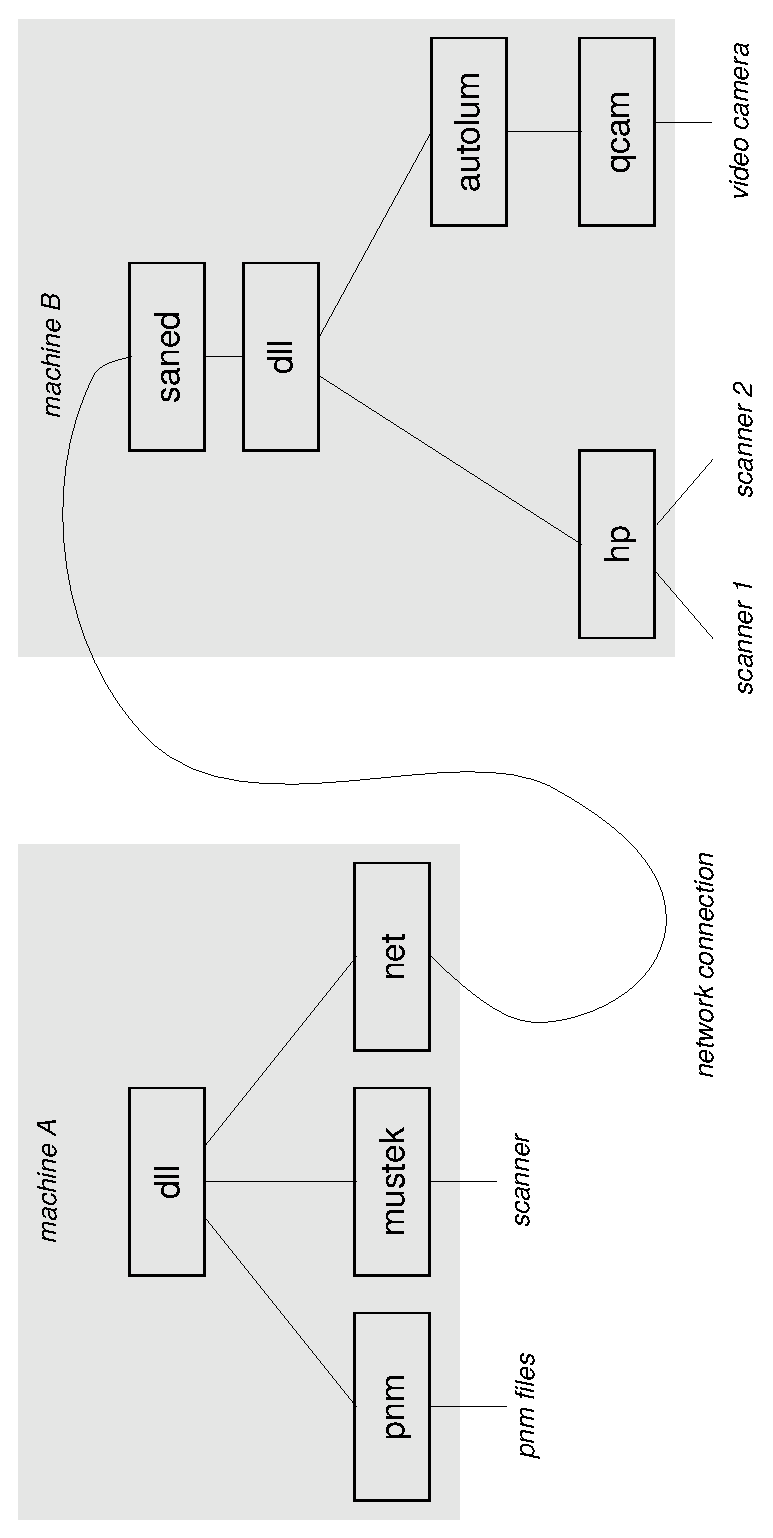
\psfig{file=figs/hierarchy.eps,angle=270,width=\textwidth}
    \caption{Example SANE Hiearchy}
    \label{fig:hierarchy}
  \end{center}
\end{figure}

The above discussion lists just a few ways for frontends to attach to
a backend.  It is of course possible to combine these solutions to
provide an entire hierarchy of SANE backends.  Such a hierarchy is
depicted in Figure~\ref{fig:hierarchy}.  The figure shows that machine
A uses a dynamic-linking based meta backend called \code{dll} to
access the backends called \code{pnm}, \code{mustek}, and \code{net}.
The first two are real backends, whereas the last one is a meta
backend that provides network transparent access to remote scanners.
In the figure, machine B provides non-local access to its scanners
through the SANE frontend called \code{saned}.  The \code{saned} in
turn has access to the \code{hp} and \code{autolum} backends through
another instance of the \code{dll} backend.  The \code{autolum} meta
backend is used to automatically adjust the luminance (brightness) of
the image data acquired by the camera backend called \code{qcam}.

Note that a meta backend really is both a frontend and a backend at
the same time.  It is a frontend from the viewpoint of the backends
that it manages and a backend from the viewpoint of the frontends that
access it.  The name ``meta backend'' was chosen primarily because the
SANE standard describes the interface from the viewpoint of a (real)
frontend.


\section{Image Data Format}\label{sec:imageformat}\index{image data format}

Arguably the most important aspect of an image acquisition system is
how images are represented.  The SANE approach is to define a simple
yet powerful representation that is sufficient for vast majority of
applications and devices.  While the representation is simple, the
interface has been defined carefully to allow extending it in the
future without breaking backwards compatibility.  Thus, it will be
possible to accommodate future applications or devices that were not
anticipated at the time this standard was created.

A SANE image is a rectangular area.  The rectangular area is
subdivided into a number of rows and columns.  At the intersection of
each row and column is a quadratic pixel.  A pixel consists of one or
more sample values.  Each sample value represents one channel (e.g.,
the red channel).  Each sample value has a certain bit depth.  The bit
depth is fixed for the entire image and can be as small as one bit.
Valid bit depths are 1, 8, or 16 bits per sample.  If a device's
natural bit depth is something else, it is up to the driver to scale
the sample values appropriately (e.g., a 4 bit sample could be scaled
by a factor of four to represent a sample value of depth 8).

\subsection{Image Transmission}

The SANE API transmits an image as a sequence of frames.  Each frame
covers the same rectangular area as the entire image, but may contain
only a subset of the channels in the final image.  For example, a
red/green/blue image could either be transmitted as a single frame
that contains the sample values for all three channels or it could be
transmitted as a sequence of three frames: the first frame containing
the red channel, the second the green channel, and the third the blue
channel.

Conceptually, each frame is transmitted a byte at a time.  Each byte
may contain 8 sample values (for an image bit depth of 1), one full
sample value (for an image bit depth of 8), or a partial sample value
(for an image bit depth of 16 or bigger).  In the latter case, the
bytes of each sample value are transmitted in the machine's native
byte order. For depth 1, the leftmost pixel is stored in the most
significant bit, and the rightmost pixel in the least significant bit.
\begin{quote}
  \begin{center}
    {\bf Backend Implementation Note}
  \end{center}
  A network-based meta backend will have to ensure that the byte order
  in image data is adjusted appropriately if necessary.  For example,
  when the meta backend attaches to the server proxy, the proxy may
  inform the backend of the server's byte order.  The backend can then
  apply the adjustment if necessary.  In essence, this implements a
  ``receiver-makes-right'' approach.
\end{quote}

\begin{figure}[htbp]
  \begin{center}
    \leavevmode
    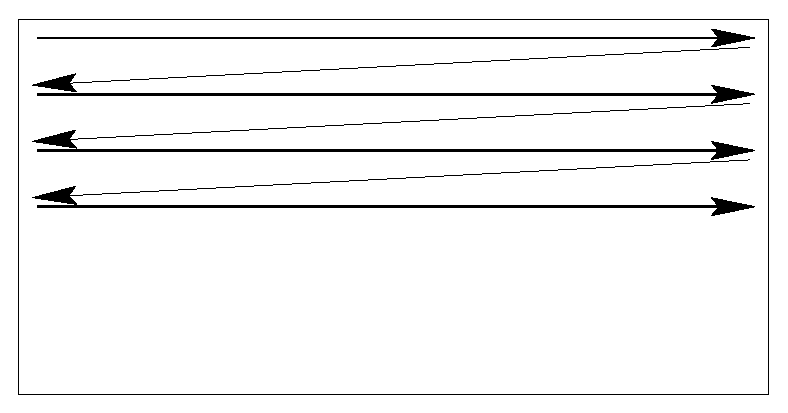
\psfig{file=figs/xfer.eps,width=0.5\textwidth}
    \caption{Transfer order of image data bytes}
    \label{fig:xfer}
  \end{center}
\end{figure}

The order in which the sample values in a frame are transmitted is
illustrated in Figure~\ref{fig:xfer}.  As can be seen, the values are
transmitted row by row and each row is transmitted from left-most to
right-most column.  The left-to-right, top-to-bottom transmission
order applies when the image is viewed in its normal orientation (as
it would be displayed on a screen, for example).

If a frame contains multiple channels, then the channels are
transmitted in an interleaved fashion.  Figure~\ref{fig:pixels}
illustrates this for the case where a frame contains a complete
red/green/blue image with a bit-depth of 8.  For a bit depth of 1,
each byte contains 8 sample values of a {\em single\/} channel.  In
other words, a bit depth 1 frame is transmitted in a byte interleaved
fashion.

\begin{figure}[htbp]
  \begin{center}
    \leavevmode
    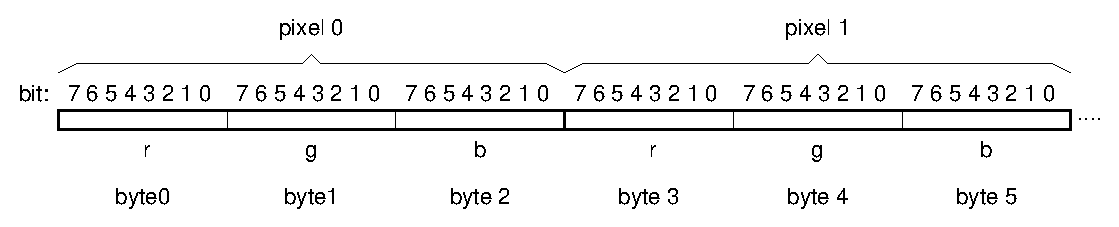
\psfig{file=figs/image-data.eps,width=0.8\textwidth}
    \caption{Bit and byte order or image data}
    \label{fig:pixels}
  \end{center}
\end{figure}

When transmitting an image frame by frame, the frontend needs to know
what part of the image a frame represents (and how many frames it
should expect).  For that purpose, the SANE API tags every frame with
a type.  This version of the SANE standard supports the following
frame types:
\begin{quote}
\begin{description}

\item[\code{\defn{SANE\_FRAME\_GRAY}}:] The frame contains a single
  channel of data that represents sample values from a spectral band
  that covers the human visual range.  The image consists of this
  frame only.

\item[\code{\defn{SANE\_FRAME\_RGB}}:] The frame contains three
  channels of data that represent sample values from the red, green,
  and blue spectral bands.  The sample values are interleaved in the
  order red, green, and blue.  The image consists of this frame only.

\item[\code{\defn{SANE\_FRAME\_RED}}:] The frame contains one channel
  of data that represents sample values from the red spectral band.
  The complete image consists of three frames:
  \code{SANE\_\-FRA\-ME\_RED}, \code{SANE\_FRAME\_GREEN}, and
  \code{SANE\_FRAME\_BLUE}.  The order in which the frames are
  transmitted chosen by the backend.

\item[\code{\defn{SANE\_FRAME\_GREEN}}:] The frame contains one
  channel of data that represents sample values from the green
  spectral band.  The complete image consists of three frames:
  \code{SANE\_\-FRA\-ME\_RED}, \code{SANE\_FRAME\_GREEN}, and
  \code{SANE\_FRAME\_BLUE}.  The order in which the frames are
  transmitted chosen by the backend.

\item[\code{\defn{SANE\_FRAME\_BLUE}}:] The frame contains one channel
  of data that represents sample values from the blue spectral band.
  The complete image consists of three frames:
  \code{SANE\_\-FRA\-ME\_RED}, \code{SANE\_FRAME\_GREEN}, and
  \code{SANE\_FRAME\_BLUE}.  The order in which the frames are
  transmitted chosen by the backend.

\end{description}
\end{quote}

In frames of type \code{SANE\_FRAME\_GRAY}, when the bit depth is 1 there are
only two sample values possible, 1 represents minimum intensity
(black) and 0 represents maximum intensity (white).  For all other bit
depth and frame type combinations, a sample value of 0 represents
minimum intensity and larger values represent increasing intensity.

The combination of bit depth 1 and \code{SANE\_FRAME\_RGB} (or
\code{SANE\_FRAME\_RED}, \code{SANE\_FRAME\_GREEN}, \code{SANE\_FRAME\_BLUE})
is rarely used and may not be supported by every frontend.

\chapter{The SANE Application Programmer Interface (API)}\label{chap:api}

This Section defines version 1 of the SANE application
programmer interface (API).  Any SANE frontend must depend on the
interface defined in this section only.  Converseley, any SANE backend
must implement its functionality in accordance with this
specification.  The interface as documented here is declared as a C
callable interface in a file called \filename{sane/sane.h}.  This file should
normally be included via a C pre-processor directive of the form:
\begin{verbatim}
  #include <sane/sane.h>
\end{verbatim}


\section{Version Control}

The SANE standard is expected to evolve over time.  Whenever a change
to the SANE standard is made that may render an existing frontend or
backend incompatible with the new standard, the major version number
must be increased.  Thus, any frontend/backend pair is compatible
provided the major version number of the SANE standard they implement
is the same.  A frontend may implement backwards compatiblity by
allowing major numbers that are smaller than the expected major number
(provided the frontend really can cope with the older version).  In
contrast, a backend always provides support for one and only one
version of the standard.  If a specific application does require that
two different versions of the same backend are accessible at the same
time, it is possible to do so by installing the two versions under
different names.

SANE version control also includes a minor version number and a build
revision.  While control of these numbers remains with the implementor
of a backend, the recommended use is as follows.  The minor version is
incremented with each official release of a backend.  The build
revision is increased with each build of a backend.

The SANE API provides the following five macros to manage version
numbers.
\begin{quote}
  \begin{description}
  \item[\code{\defn{SANE\_CURRENT\_MAJOR}}:] The value of this macro is the
    number of the SANE standard that the interface implements.

  \item[\code{\defn{SANE\_VERSION\_CODE}(\var{maj},\var{min},\var{bld})}:]
    \label{sec:saneversioncode}
    This macro can be used to build a monotonically increasing version
    code.  A SANE version code consists of the SANE standard major
    version number (\var{maj}), the minor version number \var{min},
    and the build revision of a backend (\var{bld}).  The major and
    minor version numbers must be in the range 0\ldots255 and the
    build revision must be in the range 0\ldots65535.

    Version codes are monotonic in the sense that it is possible to
    apply relational operators (e.g., equality or less-than test)
    directly on the version code rather than individually on the three
    components of the version code.

    Note that the major version number alone determines whether a
    frontend/backend pair is compatible.  The minor version and the
    build revision are used for informational and bug-fixing purposes
    only.
  
  \item[\code{\defn{SANE\_VERSION\_MAJOR}(\var{vc})}:] This macro returns the
    major version number component of the version code passed in
    argument \var{vc}.
  \item[\code{SANE\_VERSION\_MINOR(\var{vc})}:] This macro returns the
    minor version number component of the version code passed in
    argument \var{vc}.
  \item[\code{SANE\_VERSION\_BUILD(\var{vc})}:] This macro returns the
    build revision component of the version code passed in argument
    \var{vc}.
  \end{description}
\end{quote}


\section{Data Types}

\subsection{Base Types}

The SANE standard is based on just two SANE-specific base types: the
SANE byte and word.
\begin{quote}
  \code{typedef \var{some-scalar-type\/} \defn{SANE\_Byte};} \\
  \code{typedef \var{some-scalar-type\/} \defn{SANE\_Word};}
\end{quote}
\verb|SANE_Byte| must correspond to some scalar C type that is capable
of holding values in the range 0 to 255.  \verb|SANE_Word| must be
capable of holding any of the following:
\begin{itemize}
  \item the truth values \verb|SANE_FALSE| and \verb|SANE_TRUE|
  \item signed integers in the range $-2^{31}\ldots2^{31}-1$
  \item fixed point values in the range $-32768\ldots32767.9999$ with
    a resolution of $1/65536$
  \item 32 bits (for bit sets)
\end{itemize}
Note that the SANE standard does not define what C type
\verb|SANE_Byte| and \verb|SANE_Word| map to.  For example, on some
platforms, the latter may map to \verb|long int| whereas on others it
may map to \verb|int|.  A portable SANE frontend or backend must
therefore not depend on a particular mapping.

\subsection{Boolean Type}

\code{\defn{SANE\_Bool}} is used for variables that can take one of
the two truth values \code{\defn{SANE\_FALSE}} and
\code{\defn{SANE\_TRUE}}.  The former value is defined to be 0,
whereas the latter is 1.\footnote{This is different from ANSI C where
  any non-zero integer value represents logical TRUE.} The C
declarations for this type are given below.
\begin{quote}
\begin{verbatim}
#define SANE_FALSE      0
#define SANE_TRUE       1
typedef SANE_Word SANE_Bool;
\end{verbatim}
\end{quote}
Note that \verb|SANE_Bool| is simply an alias of \verb|SANE_Word|.  It
is therefore always legal to use the latter type in place of the
former.  However, for clarity, it is recommended to use
\verb|SANE_Bool| whenever a given variable or formal argument has a
fixed interpretation as a boolean object.

\subsection{Integer Type}

\code{\defn{SANE\_Int}} is used for variables that can take integer
values in the range $-2^{32}$ to $2^{31}-1$.  Its C declaration is
given below.
\begin{quote}
\begin{verbatim}
typedef SANE_Word SANE_Int;
\end{verbatim}
\end{quote}
Note that \verb|SANE_Int| is simply an alias of \verb|SANE_Word|.  It
is therefore always legal to use the latter type in place of the
former.  However, for clarity, it is recommended to use
\verb|SANE_Int| whenever a given variable or formal argument has a
fixed interpretation as an integer object.


\subsection{Fixed-point Type}

\code{\defn{SANE\_Fixed}} is used for variables that can take fixed
point values in the range $-32768$ to $32767.9999$ with a resolution
of $1/65535$.  The C declarations relating to this type are given
below.
\begin{quote}
\begin{verbatim}
#define SANE_FIXED_SCALE_SHIFT  16
typedef SANE_Word SANE_Fixed;
\end{verbatim}
\end{quote}
The macro \code{\defn{SANE\_FIXED\_SCALE\_SHIFT}} gives the location
of the fixed binary point.  This standard defines that value to be 16,
which yields a resolution of $1/65536$.

Note that \verb|SANE_Fixed| is simply an alias of \verb|SANE_Word|.
It is therefore always legal to use the latter type in place of the
former.  However, for clarity, it is recommended to use
\verb|SANE_Fixed| whenever a given variable or formal argument has a
fixed interpretation as a fixed-point object.

For convenience, SANE also defines two macros that convert fixed-point
values to and from C double floating point values.
\begin{quote}
  \begin{description}

  \item[\code{\defn{SANE\_FIX}(\var{d})}:] Returns the largest SANE
    fixed-point value that is smaller than the double value \var{d}.
    No range checking is performed.  If the value of \var{d} is out of
    range, the result is undefined.

  \item[\code{\defn{SANE\_UNFIX}(\var{w})}:] Returns the nearest
    double machine number that corresponds to fixed-point value
    \var{w}.

  \end{description}
\end{quote}
SANE does {\em not\/} require that the following two expressions hold
true (even if the values of \var{w} and \var{d} are in range):
\begin{quote}
\begin{verbatim}
SANE_UNFIX(SANE_FIX(d)) == d
SANE_FIX(SANE_UNFIX(w)) == w
\end{verbatim}
\end{quote}
In other words, conversion between fixed and double values may be
lossy.  It is therefore recommended to avoid repeated conversions
between the two representations.


\subsection{Text}

\subsubsection{Character Type}

Type \code{\defn{SANE\_Char}} represents a single text character or
symbol.  At present, this type maps directly to the underlying C
\verb|char| type (typically one byte).  The encoding for such
characters is currently fixed as ISO LATIN-1.  Future versions of this
standard may map this type to a wider type and allow multi-byte
encodings to support internationalization.  As a result of this, care
should be taken to avoid the assumption that
\verb|sizeof(SANE_Char)==sizeof(char)|.
\begin{quote}
\begin{verbatim}
typedef char SANE_Char;
\end{verbatim}
\end{quote}

\subsubsection{String Type}

Type \code{\defn{SANE\_String}} represents a text string as a sequence
of C \verb|char| values.  The end of the sequence is indicated by a
\verb|'\0'| (\defn{NUL}) character.  
\begin{quote}
\begin{verbatim}
typedef SANE_Char *SANE_String;
typedef const SANE_Char *SANE_String_Const;
\end{verbatim}
\end{quote}
The type \code{\defn{SANE\_String\_Const}} is provided by SANE to
enable declaring strings whose contents is unchangable.  Note that in
ANSI C, the declaration
\begin{quote}
\begin{verbatim}
const SANE_String str;
\end{verbatim}
\end{quote}
declares a string pointer that is constant (not a string pointer that
points to a constant value).


\subsection{Scanner Handle Type}

Access to a scanner is provided through an opaque type called
\code{\defn{SANE\_Handle}}.  The C declaration of this type is given
below.
\begin{quote}
\begin{verbatim}
typedef void *SANE_Handle;
\end{verbatim}
\end{quote}
While this type is declared to be a void pointer, an application must
not attempt to interpret the value of a \verb|SANE_Handle|.  In
particular, SANE does not require that a value of this type is a legal
pointer value.


\subsection{Status Type}

Most SANE operations return a value of type \code{\defn{SANE\_Status}}
to indicate whether the completion status of the operation.  If an
operation completes successfully, \verb|SANE_STATUS_GOOD| is returned.
In case of an error, a value is returned that indicates the nature of
the problem.  The complete list of available status codes is listed in
Table \ref{tab:status}.  It is recommended to use function
\code{sane\_strstatus()} to convert status codes into a legible
string.

\begin{table}[htbp]
  \begin{center}
    \begin{tabular}{|l|r|l|}
      \hline
      \multicolumn{1}{|c|}{\bf Symbol} & \multicolumn{1}{c|}{\bf Code} &
      \multicolumn{1}{c|}{\bf Description} \\
      \hline\hline
\code{\defn{SANE\_STATUS\_GOOD}}
        &  0 & Operation completed succesfully. \\
\code{\defn{SANE\_STATUS\_UNSUPPORTED}}
        &  1 & Operation is not supported. \\
\code{\defn{SANE\_STATUS\_CANCELLED}}
        &  2 & Operation was cancelled. \\
\code{\defn{SANE\_STATUS\_DEVICE\_BUSY}}
        &  3 & Device is busy---retry later. \\
\code{\defn{SANE\_STATUS\_INVAL}}
        &  4 & Data or argument is invalid. \\
\code{\defn{SANE\_STATUS\_EOF}}
        &  5 & No more data available (end-of-file). \\
\code{\defn{SANE\_STATUS\_JAMMED}}
        &  6 & Document feeder jammed. \\
\code{\defn{SANE\_STATUS\_NO\_DOCS}}
        &  7 & Document feeder out of documents. \\
\code{\defn{SANE\_STATUS\_COVER\_OPEN}}
        &  8 & Scanner cover is open. \\
\code{\defn{SANE\_STATUS\_IO\_ERROR}}
        &  9 & Error during device I/O. \\
\code{\defn{SANE\_STATUS\_NO\_MEM}}
        & 10 & Out of memory. \\
\code{\defn{SANE\_STATUS\_ACCESS\_DENIED}}
        & 11 & Access to resource has been denied. \\
      \hline
    \end{tabular}
    \caption{Status Codes}\label{tab:status}
  \end{center}
\end{table}


\subsection{Device Descriptor Type}

Each SANE device is represented by a structure of type
\code{\defn{SANE\_Device}}.  The C declaration of this type is given
below.
\begin{quote}
\begin{verbatim}
typedef struct
  {
    SANE_String_Const name;
    SANE_String_Const vendor;
    SANE_String_Const model;
    SANE_String_Const type;
  }
SANE_Device;
\end{verbatim}
\end{quote}
\index{device-name}
The structure provides the unique name of the scanner in member
\code{name}.  It is this unique name that should be passed in a call
to \code{sane\_open()}.  The format of this name is completely up to
the backend.  The only constraints are that the name is unique among
all devices supported by the backend and that the name is a legal SANE
text string.  To simplify presentation of unique names, their length
should not be excessive.  It is {\em recommended\/} that backends keep
unique names below 32 characters in length.  However, applications
{\em must\/} be able to cope with arbitrary length unique names.

The remaining members in the device structure provide additional
information on the device corresponding to the unique name.
Specifically, members \code{vendor}, \code{model}, and \code{type} are
single-line strings that give information on the vendor
(manufacturer), model, and the type of the device.  For consistency's
sake, the following strings should be used when appropriate (the lists
will be expanded as need arises):

\begin{table}[htbp]
  \begin{center}
    \leavevmode
    \hspace{\fill}
    \begin{tabular}[t]{|ll|}
      \hline
      \multicolumn{2}{|c|}{\bf \defn{Vendor Strings}} \\
      \hline\hline
      \code{AGFA}            & \code{Microtek} \\ 
      \code{Abaton}          & \code{Minolta} \\             
      \code{Acer}            & \code{Mitsubishi} \\  
      \code{Apple}           & \code{Mustek} \\      
      \code{Artec}           & \code{NEC} \\         
      \code{Avision}         & \code{Nikon} \\       
      \code{CANON}           & \code{Plustek} \\     
      \code{Connectix}       & \code{Polaroid} \\    
      \code{Epson}           & \code{Relisys} \\     
      \code{Fujitsu}         & \code{Ricoh} \\       
      \code{Hewlett-Packard} & \code{Sharp} \\       
      \code{IBM}             & \code{Siemens} \\     
      \code{Kodak}           & \code{Tamarack} \\    
      \code{Lexmark}	     & \code{UMAX} \\        
      \code{Logitech}        & \code{Noname} \\
      \hline
    \end{tabular}
    \hspace{\fill}
    \begin{tabular}[t]{|l|}
      \hline
      \multicolumn{1}{|c|}{\bf \defn{Type Strings}} \\
      \hline\hline
      \code{film scanner} \\
      \code{flatbed scanner} \\
      \code{frame grabber} \\
      \code{handheld scanner} \\
      \code{multi-function peripheral} \\
      \code{sheetfed scanner} \\
      \code{still camera} \\
      \code{video camera} \\
      \code{virtual device} \\
      \hline
    \end{tabular}
    \hspace{\fill}
    \caption{Predefined Device Information Strings}
    \label{tab:devinfo}
  \end{center}
\end{table}
Note that vendor string \code{Noname} can be used for virtual devices
that have no physical vendor associated.  Also, there are no
predefined model name strings since those are vendor specific and
therefore completely under control of the respective backends.


\subsection{Option Descriptor Type}\label{sec:odesc}

Option descriptors are at the same time the most intricate and
powerful type in the SANE standard.  Options are used to control
virtually all aspects of device operation.  Much of the power of the
SANE API stems from the fact that most device controls are completely
described by their respective option descriptor.  Thus, a frontend can
control a scanner abstractly, without requiring knowledge as to what
the purpose of any given option is.  Conversely, a scanner can
describe its controls without requiring knowledge of how the frontend
operates.  The C declaration of the
\code{\defn{SANE\_Option\_Descriptor}} type is given below.
\begin{quote}
\begin{verbatim}
typedef struct
  {
    SANE_String_Const name;
    SANE_String_Const title;
    SANE_String_Const desc;
    SANE_Value_Type type;
    SANE_Unit unit;
    SANE_Int size;
    SANE_Int cap;
    SANE_Constraint_Type constraint_type;
    union
      {
        const SANE_String_Const *string_list;
        const SANE_Word *word_list;
        const SANE_Range *range;
      }
    constraint;
  }
SANE_Option_Descriptor;
\end{verbatim}
\end{quote}

\subsubsection{Option Name}

Member \code{name} is a string that uniquely identifies the option.
The name must be unique for a given device (i.e., the option names
across different backends or devices need not be unique).  The option
name must consist of lower-case ASCII letters (\code{a}--\code{z}),
digits (\code{0}--\code{9}), or the dash character (\code{-}) only.
The first character must be a lower-case ASCII character (i.e., not a
digit or a dash).

\subsubsection{Option Title}

Member \code{title} is a single-line string that can be used by the
frontend as a title string.  This should typically be a short (one or
two-word) string that is chosen based on the function of the option.

\subsubsection{Option Description}

Member \code{desc} is a (potentially very) long string that can be
used as a help text to describe the option.  It is the responsibility
of the frontend to break the string into managable-length lines.
Newline characters in this string should be interpreted as paragraph
breaks.

\subsubsection{Option Value Type}

Member \code{type} specifies the type of the option value.  The
possible values for type \code{\defn{SANE\_Value\_Type}} are described
in Table \ref{tab:valuetype}.

\begin{table}[htbp]
  \begin{center}
    \leavevmode
    \begin{tabular}{|l|l|p{0.6\textwidth}|}
\hline
\multicolumn{1}{|c|}{\bf Symbol} &
\multicolumn{1}{c|}{\bf Code} &
\multicolumn{1}{c|}{\bf Description} \\
\hline\hline

\code{\defn{SANE\_TYPE\_BOOL}} & 0 & Option value is of type
  \verb|SANE_Bool|. \\ 

\code{\defn{SANE\_TYPE\_INT}} & 1 & Option value is of type
  \verb|SANE_Int|. \\ 

\code{\defn{SANE\_TYPE\_FIXED}}&2 & Option value is of type
  \verb|SANE_Fixed|. \\ 

\code{\defn{SANE\_TYPE\_STRING}}&3 & Option value is of type
  \verb|SANE_String|. \\ 

\code{\defn{SANE\_TYPE\_BUTTON}} & 4 & An option of this type has no value.
Instead, setting an option of this type has an option-specific
side-effect.  For example, a button-typed option could be used by a
backend to provide a means to select default values or to the tell an
automatic document feeder to advance to the next sheet of paper. \\ 

\code{\defn{SANE\_TYPE\_GROUP}} & 5 & An option of this type has no value.
This type is used to group logically related options.  A group option
is in effect up to the point where another group option is encountered
(or up to the end of the option list, if there are no other group
options).  For group options, only members \code{title} and
\code{type} are valid in the option descriptor. \\ 

  \hline
    \end{tabular}
    \caption{Option Value Types (\code{SANE\_Value\_Type})}
    \label{tab:valuetype}
  \end{center}
\end{table}

\subsubsection{Option Value Unit}

Member \code{unit} specifies what the physical unit of the option
value is.  The possible values for type \code{\defn{SANE\_U\-nit}} are
described in Table \ref{tab:units}.  Note that the specified unit is
what the SANE backend expects.  It is entirely up to a frontend as to
how these units a presented to the user.  For example, SANE expresses
all lengths in millimeters.  A frontend is generally expected to
provide appropriate conversion routines so that a user can express
quantities in a customary unit (e.g., inches or centimeters).

\begin{table}[htbp]
  \begin{center}
    \leavevmode
    \begin{tabular}{|l|l|l|}
\hline
\multicolumn{1}{|c|}{\bf Symbol} &
\multicolumn{1}{|c|}{\bf Code} &
\multicolumn{1}{|c|}{\bf Description} \\

\hline\hline

\code{\defn{SANE\_UNIT\_NONE}}   & 0 & Value is unit-less (e.g., page count).\\
\code{\defn{SANE\_UNIT\_PIXEL}}  & 1 & Value is in number of pixels. \\
\code{\defn{SANE\_UNIT\_BIT}}    & 2 & Value is in number of bits. \\
\code{\defn{SANE\_UNIT\_MM}}     & 3 & Value is in millimeters. \\
\code{\defn{SANE\_UNIT\_DPI}}    & 4 & Value is a resolution in dots/inch. \\
\code{\defn{SANE\_UNIT\_PERCENT}}& 5 & Value is a percentage. \\
\code{\defn{SANE\_UNIT\_MICROSECOND}}& 6 & Value is time in $\mu$-seconds. \\

\hline
    \end{tabular}
    \caption{Physical Units (\code{SANE\_Unit})}
    \label{tab:units}
  \end{center}
\end{table}

\subsubsection{Option Value Size}\label{sec:valuesize}

Member \code{size} specifies the size of the option value (in bytes).
This member has a slightly different interpretation depending on the
type of the option value:
\begin{quote}
  \begin{description}
  \item[\code{SANE\_TYPE\_STRING}:] The size is the maximum size of
    the string.  For the purpose of string size calcuations, the
    terminating \code{NUL} character is considered to be part of the
    string.  Note that the terminating \code{NUL} character must
    always be present in string option values.
  \item[\code{SANE\_TYPE\_INT}, \code{SANE\_TYPE\_FIXED}:] The size
    must be a positive integer multiple of the size of a
    \verb|SANE_Word|.  The option value is a vector of length
    \[ \code{size}/\code{sizeof(SANE\_Word)}. \]
  \item[\code{SANE\_TYPE\_BOOL}:] The size must be set to
    \code{sizeof(SANE\_Word)}.
  \item[\code{SANE\_TYPE\_BUTTON}, \code{SANE\_TYPE\_GROUP}:] The
    option size is ignored.
  \end{description}
\end{quote}

\subsubsection{Option Capabilities}

Member \code{cap} describes what capabilities the option posseses.
This is a bitset that is formed as the inclusive logical OR of the
capabilities described in Table \ref{tab:capabilities}.  The SANE API
provides the following to macros to test certain features of a given
capability bitset:
\begin{quote}
  \begin{description}

  \item[\code{\defn{SANE\_OPTION\_IS\_ACTIVE}(\var{cap})}:] This macro
    returns \code{SANE\_TRUE} if and only if the option with the
    capability set \var{cap} is currently active.

  \item[\code{\defn{SANE\_OPTION\_IS\_SETTABLE}(\var{cap})}:] This
    macro returns \code{SANE\_TRUE} if and only if the option with the
    capability set \var{cap} is software settable.
  \end{description}
\end{quote}

\begin{table}[htbp]
  \begin{center}
    \leavevmode
    \begin{tabular}{|l|r|p{0.59\textwidth}|}
\hline
\multicolumn{1}{|c|}{\bf Symbol} &
\multicolumn{1}{c|}{\bf Code} &
\multicolumn{1}{c|}{\bf Description} \\
\hline\hline

\code{\defn{SANE\_CAP\_SOFT\_SELECT}} & 1 & The option
  value can be set by a call to \code{sane\_con\-trol\_opt\-ion()}.\\ 

\code{\defn{SANE\_CAP\_HARD\_SELECT}} & 2 & The option value can be set by
  user-intervention (e.g., by flipping a switch).  The user-interface
  should prompt the user to execute the appropriate action to set such
  an option.  This capability is mutually exclusive with
  SANE\_CAP\_SOFT\_SELECT (either one of them can be set, but not both
  simultaneously).  \\ 

\code{\defn{SANE\_CAP\_SOFT\_DETECT}} & 4 & The option
  value can be detected by software.  If
  \code{SANE\_\-CAP\_\-SO\-FT\_SEL\-ECT} is set, this capability {\em must\/}
  be set.  If \code{SANE\_CAP\_HARD\_SELECT} is set, this capability
  may or may not be set.  If this capability is set but neither
  \code{SANE\_CAP\_SO\-FT\_SEL\-ECT} nor \code{SANE\_CAP\_HA\-RD\_SEL\-ECT}
  are, then there is no way to control the option.  That is, the
  option provides read-out of the current value only.  \\ 

\code{\defn{SANE\_CAP\_EMULATED}} & 8 & If set, this capability indicates
  that an option is not directly supported by the device and is
  instead emulated in the backend.  A sophisticated frontend may
  elect to use its own (presumably better) emulation in lieu of an emulated
  option. \\ 

\code{\defn{SANE\_CAP\_AUTOMATIC}} & 16 & If set, this capability indicates
  that the backend (or the device) is capable to picking a reasonable
  option value automatically.  For such options, it is possible to
  select automatic operation by calling \code{sane\_control\_option()}
  with an action value of \code{SANE\_ACTION\_SET\_AUTO}.  \\ 

\code{\defn{SANE\_CAP\_INACTIVE}} & 32 & If set, this capability indicates
  that the option is not currently active (e.g., because it's
  meaningful only if another option is set to some other value). \\ 

\code{\defn{SANE\_CAP\_ADVANCED}} & 64 &
  If set, this capability indicates that the option should be
  considered an ``advanced user option.''  A frontend typically
  displays such options in a less conspicuous way than regular options
  (e.g., a command line interface may list such options last or a
  graphical interface may make them available in a seperate ``advanced
  settings'' dialog). 
  \\

\hline
    \end{tabular}
    \caption{Option Capabilities}
    \label{tab:capabilities}
  \end{center}
\end{table}

\subsubsection{Option Value Constraints}

It is often useful to constrain the values that an option can take.
For example, constraints can be used by a frontend to determine how to
represent a given option.  Member \code{constraint\_type} indicates
what constraint is in effect for the option.  The constrained values
that are allowed for the option are described by one of the union
members of member \code{constraint}.  The possible values of type
\code{\defn{SANE\_Constraint\_Type}} and the interpretation of the
\code{constraint} union is described in Table~\ref{tab:constraints}.

\begin{table}[htbp]
  \begin{center}
    \leavevmode
    \begin{tabular}{|l|r|p{0.5\textwidth}|}
\hline
\multicolumn{1}{|c|}{\bf Symbol} &
\multicolumn{1}{|c|}{\bf Code} &
\multicolumn{1}{|c|}{\bf Description} \\

\hline\hline

\code{\defn{SANE\_CONSTRAINT\_NONE}} & 0 & The value is unconstrained.
  The option can take any of the values possible for the option's
  type. \\

  \code{\defn{SANE\_CONSTRAINT\_RANGE}} & 1 & This constraint is
  applicable to integer and fixed-point valued options only.  It
  constrains the option value to a possibly quantized range of
  numbers.  Option descriptor member \code{constraint.range} points to
  a range of the type \code{\defn{SANE\_Range}}.  This type is illustrated
  below:
  \begin{quote}
\begin{verbatim}
typedef struct
  {
    SANE_Word min;
    SANE_Word max;
    SANE_Word quant;
  }
SANE_Range;
\end{verbatim}
  \end{quote}
  All three members in this structure are interpreted according to the
  option value type (\verb|SANE_TYPE_INT| or \verb|SANE_TYPE_FIXED|).
  Members \code{min} and \code{max} specify the minimum and maximum
  values, respectively.  If member \code{quant} is non-zero, it
  specifies the quantization value.  If $l$ is the minimum value, $u$
  the maximum value and $q$ the (non-zero) quantization of a range,
  then the legal values are $v=k\cdot q+l$ for all non-negative
  integer values of $k$ such that $v<=u$.  \\ 

\code{\defn{SANE\_CONSTRAINT\_WORD\_LIST}} & 2 & This constraint is applicable
  to integer and fixed-point valued options only.  It constrains the
  option value to a list of numeric values.  Option descriptor member
  \code{constraint.word\_list} points to a list of words that
  enumerates the legal values.  The first element in that list is an
  integer (\verb|SANE_Int|) that specifies the length of the list (not
  counting the length itself).  The remaining elements in the list are
  interpreted according to the type of the option value
  (\verb|SANE_TYPE_INT| or \verb|SANE_TYPE_FIXED|). \\ 

\code{\defn{SANE\_CONSTRAINT\_STRING\_LIST}} & 3 & This constraint is
  applicable to string-valued options only.  It constrains the option
  value to a list of strings.  The option descriptor member
  \code{con\-strai\-nt.str\-ing\_list} points to a \code{NULL} terminated
  list of strings that enumerate the legal values for the option
  value.
\\\hline
    \end{tabular}
    \caption{Option Value Constraints}
    \label{tab:constraints}
  \end{center}
\end{table}


\section{Operations}

\subsection{\code{sane\_init}}

This function must be called before any other SANE function can be called.
The behavior of a SANE backend is undefined if this function is not called
first or if the status code returned by \code{sane\_init} is different from
\code{\defn{SANE\_STATUS\_GOOD}}.  The version code of the backend is returned
in the value pointed to by \code{version\_code}.  If that pointer is
\code{NULL}, no version code is returned.  Argument \code{authorize} is either
a pointer to a function that is invoked when the backend requires
authentication for a specific resource or \code{NULL} if the frontend does not
support authentication.
\begin{quote}\index{sane\_init}
\begin{verbatim}
SANE_Status sane_init (SANE_Int * version_code,
                       SANE_Authorization_Callback authorize);
\end{verbatim}
\end{quote}

The authorization function may be called by a backend in response to
any of the following calls:
\begin{quote}
  \code{sane\_open}, \code{sane\_control\_option}, \code{sane\_start}
\end{quote}
If a backend was initialized without authorization function, then
authorization requests that cannot be handled by the backend itself
will fail automatically and the user may be prevented from accessing
protected resources.  Backends are encouraged to implement means of
authentication that do not require user assistance.  E.g., on a
multi-user system that authenticates users through a login process a
backend could automatically lookup the apporpriate password based on
resource- and user-name.

The authentication function type has the following declaration:
\begin{quote}\index{SANE\_Authorization\_Callback}
  \index{domain}\index{username}\index{password}
\begin{verbatim}
#define SANE_MAX_USERNAME_LEN   128
#define SANE_MAX_PASSWORD_LEN   128

typedef void (*SANE_Authorization_Callback)
    (SANE_String_Const resource,
     SANE_Char username[SANE_MAX_USERNAME_LEN],
     SANE_Char password[SANE_MAX_PASSWORD_LEN]);
\end{verbatim}
\end{quote}
Three arguments are passed to the authorization function:
\code{resource} is a string specifying the name of the resource that
requires authorization.  A frontend should use this string to build a
user-prompt requesting a username and a password.  The \code{username}
and \code{password} arguments are (pointers to) an array of
\code{SANE\_MAX\_USERNAME\_LEN} and \code{SANE\_MAX\_PASSWORD\_LEN}
characters, respectively.  The authorization call should place the
entered username and password in these arrays.  The returned strings
{\em must\/} be ASCII-NUL terminated.

\subsection{\code{sane\_exit}}

This function must be called to terminate use of a backend.  The
function will first close all device handles that still might be open
(it is recommended to close device handles explicitly through a call
to \code{sane\_clo\-se()}, but backends are required to release all
resources upon a call to this function).  After this function returns,
no function other than \code{sane\_init()} may be called (regardless
of the status value returned by \code{sane\_exit()}.  Neglecting to
call this function may result in some resources not being released
properly.
\begin{quote}\index{sane\_exit}
\begin{verbatim}
void sane_exit (void);
\end{verbatim}
\end{quote}


\subsection{\code{sane\_get\_devices}}

This function can be used to query the list of devices that are
available.  If the function executes successfully, it stores a pointer
to a \code{NULL} terminated array of pointers to \verb|SANE_Device|
structures in \code{*device\_list}.  The returned list is guaranteed
to remain unchanged and valid until (a) another call to this function
is performed or (b) a call to \code{sane\_exit()} is performed.  This
function can be called repeatedly to detect when new devices become
available.  If argument \code{local\_only} is true, only local devices
are returned (devices directly attached to the machine that SANE is
running on).  If it is false, the device list includes all remote
devices that are accessible to the SANE library.
\begin{quote}\index{sane\_get\_devices}
\begin{verbatim}
SANE_Status sane_get_devices (const SANE_Device *** device_list,
                              SANE_Bool local_only);
\end{verbatim}
\end{quote}

This function may fail with \code{SANE\_STATUS\_NO\_MEM} if an
insufficient amount of memory is available.

\begin{quote}
  \begin{center}
    {\bf Backend Implementation Note}
  \end{center}
  SANE does not require that this function is called before a
  \code{sane\_open()} call is performed.  A device name may be
  specified explicitly by a user which would make it unnecessary and
  undesirable to call this function first.
\end{quote}


\subsection{\code{sane\_open}}

This function is used to establish a connection to a particular
device.  The name of the device to be opened is passed in argument
\code{name}.  If the call completes successfully, a handle for the
device is returned in \code{*h}.  As a special case, specifying a
zero-length string as the device requests opening the first available
device (if there is such a device).
\begin{quote}\index{sane\_open}
\begin{verbatim}
SANE_Status sane_open (SANE_String_Const name, SANE_Handle * h);
\end{verbatim}
\end{quote}

This function may fail with one of the following status codes.
\begin{quote}
\begin{description}
\item[\code{SANE\_STATUS\_DEVICE\_BUSY}:] The device is currently
  busy (in use by somebody else).
\item[\code{SANE\_STATUS\_INVAL}:] The device name is not valid.
\item[\code{SANE\_STATUS\_IO\_ERROR}:] An error occured while
  communicating with the device.
\item[\code{SANE\_STATUS\_NO\_MEM}:] An insufficent amount of memory
  is available.
\item[\code{SANE\_STATUS\_ACCESS\_DENIED}:] Access to the device has
  been denied due to insufficient or invalid authentication.
\end{description}
\end{quote}


\subsection{\code{sane\_close}}

This function terminates the association between the device handle
passed in argument \code{h} and the device it represents.  If the
device is presently active, a call to \code{sane\_cancel()} is
performed first.  After this function returns, handle \code{h} must
not be used anymore.

\begin{quote}\index{sane\_close}
\begin{verbatim}
void sane_close (SANE_Handle h);
\end{verbatim}
\end{quote}

\subsection{\code{sane\_get\_option\_descriptor}}

This function is used to access option descriptors.  The function
returns the option descriptor for option number \code{n} of the device
represented by handle \code{h}.  Option number 0 is guaranteed to be a
valid option.  Its value is an integer that specifies the number of
options that are available for device handle \code{h} (the count
includes option 0).  If $n$ is not a valid option index, the function
returns \code{NULL}.  The returned option descriptor is guaranteed to
remain valid (and at the returned address) until the device is closed.

\begin{quote}\index{sane\_get\_option\_descriptor}
\begin{verbatim}
const SANE_Option_Descriptor *
    sane_get_option_descriptor (SANE_Handle h, SANE_Int n);
\end{verbatim}
\end{quote}

\subsection{\code{sane\_control\_option}}\label{sec:control}

This function is used to set or inquire the current value of option
number \code{n} of the device represented by handle \code{h}.  The
manner in which the option is controlled is specified by parameter
\code{a}.  The possible values of this parameter are described in more
detail below.  The value of the option is passed through argument
\code{v}.  It is a pointer to the memory that holds the option value.
The memory area pointed to by \code{v} must be big enough to hold the
entire option value (determined by member \code{size} in the
corresponding option descriptor).  The only exception to this rule is
that when setting the value of a string option, the string pointed to
by argument \code{v} may be shorter since the backend will stop
reading the option value upon encountering the first \code{NUL}
terminator in the string.  If argument \code{i} is not \code{NULL},
the value of \code{*i} will be set to provide details on how well the
request has been met.  The meaning of this argument is described in
more detail below.
\begin{quote}\index{sane\_control\_option}
\begin{verbatim}
SANE_Status sane_control_option (SANE_Handle h, SANE_Int n,
                                 SANE_Action a, void *v,
                                 SANE_Int * i);
\end{verbatim}
\end{quote}

The way the option is affected by a call to this function is
controlled by parameter \code{a} which is a value of type
\code{\defn{SANE\_Action}}.  The possible values and their meaning is
described in Table~\ref{tab:actions}.

\begin{table}[h]
  \begin{center}
    \leavevmode
    \begin{tabular}{|l|r|p{0.5\textwidth}|}
\hline
\multicolumn{1}{|c|}{\bf Symbol} &
\multicolumn{1}{|c|}{\bf Code} &
\multicolumn{1}{|c|}{\bf Description} \\

\hline\hline

\code{\defn{SANE\_ACTION\_GET\_VALUE}} & 0 & Get current option value. \\

\code{\defn{SANE\_ACTION\_SET\_VALUE}} & 1 & Set option value.  The
  option value passed through argument \code{v} may be modified by the
  backend if the value cannot be set exactly.  \\ 

\code{\defn{SANE\_ACTION\_SET\_AUTO}} & 2 & Turn on automatic mode.  Backend
  or device will automatically select an appropriate value.  This mode
  remains effective until overridden by an explicit set value request.
  The value of parameter \code{v} is completely ignored in this case and
  may be \code{NULL}.  \\

\hline
    \end{tabular}
    \caption{Action Values (\code{SANE\_Action})}
    \label{tab:actions}
  \end{center}
\end{table}

After setting a value via an action value of
\verb|SANE_ACTION_SET_VALUE|, additional information on how well the
request has been met is returned in \code{*i} (if \code{i} is
non-\code{NULL}).  The returned value is a bitset that may contain any
combination of the values described in Table~\ref{tab:info}.
\begin{table}[htbp]
  \begin{center}
    \leavevmode
    \begin{tabular}{|l|r|p{0.5\textwidth}|}
\hline
\multicolumn{1}{|c|}{\bf Symbol} &
\multicolumn{1}{|c|}{\bf Code} &
\multicolumn{1}{|c|}{\bf Description} \\

\hline\hline

\code{\defn{SANE\_INFO\_INEXACT}} & 1 & This value is returned when
  setting an option value resulted in a value being selected that does
  not exactly match the requested value.  For example, if a scanner
  can adjust the resolution in increments of 30dpi only, setting the
  resolution to 307dpi may result in an actual setting of 300dpi.
  When this happens, the bitset returned in \code{*i} has this member
  set.  In addition, the option value is modified to reflect the
  actual (rounded) value that was used by the backend.  Note that
  inexact values are admissible for strings as well.  A backend may
  choose to ``round'' a string to the closest matching legal string
  for a constrained string value. \\

  \code{\defn{SANE\_INFO\_RELOAD\_OPTIONS}} & 2 & The setting of an
  option may affect the value or availability of one or more {\em
    other\/} options.  When this happens, the SANE backend sets this
  member in \code{*i} to indicate that the application should reload
  all options.  This member may be set if and only if at least one
  option changed. \\

\code{\defn{SANE\_INFO\_RELOAD\_PARAMS}} & 4 & The setting of an option may
  affect the parameter values (see \code{sane\_get\_parameters()}).
  If setting an option affects the parameter values, this member will
  be set in \code{*i}.  Note that this member may be set even if the
  parameters did not actually change.  However, it is guaranteed that
  the parameters never change without this member being set. \\

\hline
    \end{tabular}
    \caption{Additional Information Returned When Setting an Option}
    \label{tab:info}
  \end{center}
\end{table}

This function may fail with one of the following status codes.
\begin{quote}
\begin{description}
\item[\code{SANE\_STATUS\_UNSUPPORTED}:] The operation is not
  supported for the specified handle and option number.
\item[\code{SANE\_STATUS\_INVAL}:] The option value is not valid.
\item[\code{SANE\_STATUS\_IO\_ERROR}:] An error occured while
  communicating with the device.
\item[\code{SANE\_STATUS\_NO\_MEM}:] An insufficent amount of memory
  is available.
\item[\code{SANE\_STATUS\_ACCESS\_DENIED}:] Access to the option has
  been denied due to insufficient or invalid authentication.
\end{description}
\end{quote}



\subsection{\code{sane\_get\_parameters}}

This function is used to obtain the current scan parameters.  The
returned parameters are guaranteed to be accurate between the time a
scan has been started (\code{sane\_start()} has been called) and the
completion of that request.  Outside of that window, the returned
values are best-effort estimates of what the parameters will be when
\code{sane\_start()} gets invoked.  Calling this function before a
scan has actually started allows, for example, to get an estimate of
how big the scanned image will be.  The parameters passed to this
function are the handle \code{h} of the device for which the
parameters should be obtained and a pointer \code{p} to a parameter
structure.  The parameter structure is described in more detail below.

\begin{quote}\index{sane\_get\_parameters}
\begin{verbatim}
SANE_Status sane_get_parameters (SANE_Handle h,
                                 SANE_Parameters * p);
\end{verbatim}
\end{quote}

The scan parameters are returned in a structure of type
\code{\defn{SANE\_Parameters}}.  The C declaration of this structure
is given below.
\begin{quote}
\begin{verbatim}
typedef struct
  {
    SANE_Frame format;
    SANE_Bool last_frame;
    SANE_Int bytes_per_line;
    SANE_Int pixels_per_line;
    SANE_Int lines;
    SANE_Int depth;
  }
SANE_Parameters;
\end{verbatim}
\end{quote}

Member \code{format} specifies the format of the next frame to be
returned.  The possible values for type \code{\defn{SANE\_Frame}} are
described in Table~\ref{tab:frameformat}.  The meaning of these
values is described in more detail in Section~\ref{sec:imageformat}.
\begin{table}[htbp]
  \begin{center}
    \leavevmode
    \begin{tabular}{|l|r|l|}
\hline
\multicolumn{1}{|c|}{\bf Symbol} &
\multicolumn{1}{|c|}{\bf Code} &
\multicolumn{1}{|c|}{\bf Description} \\

\hline\hline

\code{\defn{SANE\_FRAME\_GRAY}} & 0 & Band covering human visual range. \\
\code{\defn{SANE\_FRAME\_RGB}} & 1 & Pixel-interleaved red/green/blue bands. \\
\code{\defn{SANE\_FRAME\_RED}} & 2 & Red band of a red/green/blue image. \\
\code{\defn{SANE\_FRAME\_GREEN}} & 3 & Green band of a red/green/blue image. \\
\code{\defn{SANE\_FRAME\_BLUE}} & 4 & Blue band of a red/green/blue image. \\

\hline
    \end{tabular}
    \caption{Frame Format (\code{SANE\_Frame})}
    \label{tab:frameformat}
  \end{center}
\end{table}

Member \code{last\_frame} is set to \code{SANE\_TRUE} if and only if
the frame that is currently being acquired (or the frame that will be
acquired next if there is no current frame) is the last frame of a
multi frame image (e.g., the current frame is the blue component of a
red, green, blue image).

Member \code{lines} specifies how many scan lines the frame is
comprised of.  If this value is -1, the number of lines is not known a
priori and the frontend should call \code{sane\_read()} until it
returns a status of \code{SANE\_STATUS\_EOF}.

Member \code{bytes\_per\_line} specifies the number of bytes that
comprise one scan line.

Member \code{depth} specifies the number of bits per sample.

Member \code{pixels\_per\_line} specifies the number of pixels that
comprise one scan line.

Assume $B$ is the number of channels in the frame, then the bit depth
$d$ (as given by member \code{depth}) and the number of pixels per
line $n$ (as given by this member \code{pixels\_per\_line}) are
related to $c$, the number of bytes per line (as given by member
\code{bytes\_per\_line}) as follows:
\[
  c >= \left\{
  \begin{array}{ll}
    B\cdot \lfloor (n + 7) / 8\rfloor & \mbox{if $d=1$}\\
    B\cdot n \cdot d / 8 & \mbox{if $d>1$}
  \end{array}
  \right.
\]
Note that the number of bytes per line can be larger than the minimum
value imposed by the right side of this equation.  A frontend must be
able to properly cope with such ``padded'' image formats.


\subsection{\code{sane\_start}}

This function initiates aquisition of an image from the device
represented by handle \code{h}.
\begin{quote}\index{sane\_start}
\begin{verbatim}
SANE_Status sane_start (SANE_Handle h);
\end{verbatim}
\end{quote}
This function may fail with one of the following status codes.
\begin{quote}
\begin{description}
\item[\code{SANE\_STATUS\_CANCELLED}:] The operation was cancelled through
  a call to \code{sane\_cancel}.
\item[\code{SANE\_STATUS\_DEVICE\_BUSY}:] The device is busy. The
  operation should be retried later.
\item[\code{SANE\_STATUS\_JAMMED}:] The document feeder is jammed.
\item[\code{SANE\_STATUS\_NO\_DOCS}:] The document feeder is out of
  documents.
\item[\code{SANE\_STATUS\_COVER\_OPEN}:] The scanner cover is open.
\item[\code{SANE\_STATUS\_IO\_ERROR}:] An error occurred while communicating
  with the device.
\item[\code{SANE\_STATUS\_NO\_MEM}:] An insufficent amount of memory
  is available.
\item[\code{SANE\_STATUS\_INVAL}:] The scan cannot be started with the current
  set of options. The frontend should reload the option descriptors, as if
  \code{\defn{SANE\_INFO\_RELOAD\_OPTIONS}} had been returned from a call to
  \code{sane\_control\_option()}, since the device's capabilities may have
  changed.
\end{description}
\end{quote}


\subsection{\code{sane\_read}}

This function is used to read image data from the device represented
by handle \code{h}.  Argument \code{buf} is a pointer to a memory area
that is at least \code{maxlen} bytes long.  The number of bytes
returned is stored in \code{*len}.  A backend must set this to zero
when a status other than \code{SANE\_STA\-TUS\_GOOD} is returned.
When the call succeeds, the number of bytes returned can be anywhere in
the range from 0 to \code{maxlen} bytes.
\begin{quote}\index{sane\_read}
\begin{verbatim}
SANE_Status sane_read (SANE_Handle h, SANE_Byte * buf,
                       SANE_Int maxlen, SANE_Int * len);
\end{verbatim}
\end{quote}
If this function is called when no data is available, one of two
things may happen, depending on the I/O mode that is in effect for
handle \code{h}.
\begin{enumerate}
\item If the device is in blocking I/O mode (the default mode), the
  call blocks until at least one data byte is available (or until some
  error occurs).

\item If the device is in non-blocking I/O mode, the call returns
  immediately with status \code{SANE\_STA\-TUS\_GOOD} and with
  \code{*len} set to zero.
\end{enumerate}
The I/O mode of handle \code{h} can be set via a call to
\code{sane\_set\_io\_mode()}.

This function may fail with one of the following status codes.
\begin{quote}
\begin{description}
\item[\code{SANE\_STATUS\_CANCELLED}:] The operation was cancelled through
  a call to \code{sane\_cancel}.
\item[\code{SANE\_STATUS\_EOF}:] No more data is available for the
  current frame.
\item[\code{SANE\_STATUS\_JAMMED}:] The document feeder is jammed.
\item[\code{SANE\_STATUS\_NO\_DOCS}:] The document feeder is out of
  documents.
\item[\code{SANE\_STATUS\_COVER\_OPEN}:] The scanner cover is open.
\item[\code{SANE\_STATUS\_IO\_ERROR}:] An error occurred while communicating
  with the device.
\item[\code{SANE\_STATUS\_NO\_MEM}:] An insufficent amount of memory
  is available.
\item[\code{SANE\_STATUS\_ACCESS\_DENIED}:] Access to the device has
  been denied due to insufficient or invalid authentication.
\end{description}
\end{quote}


\subsection{\code{sane\_cancel}}

This function is used to immediately or as quickly as possible cancel
the currently pending operation of the device represented by handle
\code{h}.
\begin{quote}\index{sane\_cancel}
\begin{verbatim}
void sane_cancel (SANE_Handle h);
\end{verbatim}
\end{quote}
This function can be called at any time (as long as handle \code{h} is
a valid handle) but usually affects long-running operations only (such
as image is acquisition).  It is safe to call this function
asynchronously (e.g., from within a signal handler).  It is important
to note that completion of this operaton does {\em not\/} imply that
the currently pending operation has been cancelled.  It only
guarantees that cancellation has been {\em initiated}.  Cancellation
completes only when the cancelled call returns (typically with a
status value of \code{SANE\_STATUS\_CANCELLED}).  Since the SANE API
does not require any other operations to be re-entrant, this implies
that a frontend must {\em not\/} call any other operation until the
cancelled operation has returned.


\subsection{\code{sane\_set\_io\_mode}}

This function is used to set the I/O mode of handle \code{h}.  The I/O mode
can be either blocking or non-blocking.  If argument \code{m} is
\code{SANE\_TRUE}, the mode is set to non-blocking mode, otherwise it's set to
blocking mode.  This function can be called only after a call to
\code{sane\_start()} has been performed.
\begin{quote}\index{sane\_set\_io\_mode}
\begin{verbatim}
SANE_Status sane_set_io_mode (SANE_Handle h, SANE_Bool m);
\end{verbatim}
\end{quote}
By default, newly opened handles operate in blocking mode.  A backend
may elect not to support non-blocking I/O mode.  In such a case the
status value \code{SANE\_STATUS\_UNSUPPORTED} is returned.  Blocking
I/O must be supported by all backends, so calling this function with
argument \code{m} set to \code{SANE\_FALSE} is guaranteed to complete
successfully.

This function may fail with one of the following status codes:
\begin{quote}
\begin{description}
\item[\code{SANE\_STATUS\_INVAL}:] No image acquisition is pending.
\item[\code{SANE\_STATUS\_UNSUPPORTED}:] The backend does not support
  the requested I/O mode.
\end{description}
\end{quote}


\subsection{\code{sane\_get\_select\_fd}}

This function is used to obtain a (platform-specific) file-descriptor
for handle \code{h} that is readable if and only if image data is
available (i.e., when a call to \code{sane\_read()} will return at
least one byte of data).  If the call completes successfully, the
select file-descriptor is returned in \code{*fd}.
\begin{quote}\index{sane\_get\_select\_fd}
\begin{verbatim}
SANE_Status sane_get_select_fd (SANE_Handle h, SANE_Int *fd);
\end{verbatim}
\end{quote}
This function can be called only after a call to \code{sane\_start()}
has been performed and the returned file-descriptor is guaranteed to
remain valid for the duration of the current image acquisition (i.e.,
until \code{sane\_cancel()} or \code{sane\_start()} get called again
or until \code{sane\_read()} returns with status
\code{SANE\_STA\-TUS\_EOF}).  Indeed, a backend must guarantee to
close the returned select file descriptor at the point when the next
\code{sane\_read()} call would return \code{SANE\_STA\-TUS\_EOF}.
This is necessary to ensure the application can detect when this
condition occurs without actually having to call \code{sane\_read()}.

A backend may elect not to support this operation.  In such a case,
the function returns with status code
\code{SANE\_STATUS\_UNSUPPORTED}.

Note that the only operation supported by the returned file-descriptor
is a host operating-system dependent test whether the file-descriptor
is readable (e.g., this test can be implemented using \code{select()}
or \code{poll()} under UNIX).  If any other operation is performed on
the file descriptor, the behavior of the backend becomes
unpredictable.  Once the file-descriptor signals ``readable'' status,
it will remain in that state until a call to \code{sane\_read()} is
performed.  Since many input devices are very slow, support for this
operation is strongly encouraged as it permits an application to do
other work while image acquisition is in progress.

This function may fail with one of the following status codes:
\begin{quote}
\begin{description}
\item[\code{SANE\_STATUS\_INVAL}:] No image acquisition is pending.
\item[\code{SANE\_STATUS\_UNSUPPORTED}:] The backend does not support
  this operation.
\end{description}
\end{quote}


\subsection{\code{sane\_strstatus}}

This function can be used to translate a SANE status code into a
printable string.  The returned string is a single line of text that
forms a complete sentence, but without the trailing period
(full-stop).  The function is guaranteed to never return \code{NULL}.
The returned pointer is valid at least until the next call to this
function is performed.
\begin{quote}\index{sane\_strstatus}
\begin{verbatim}
const SANE_String_Const sane_strstatus (SANE_Status status);
\end{verbatim}
\end{quote}

\section{Code Flow}\index{code flow}

The code flow for the SANE API is illustrated in
Figure~\ref{fig:flow}.  Functions \code{sane\_init()} and
\code{sane\_exit()} initialize and exit the backend, respectively.
All other calls must be performed after initialization and before
exiting the backend.

\begin{figure}[htb]
  \begin{center}
    \leavevmode
    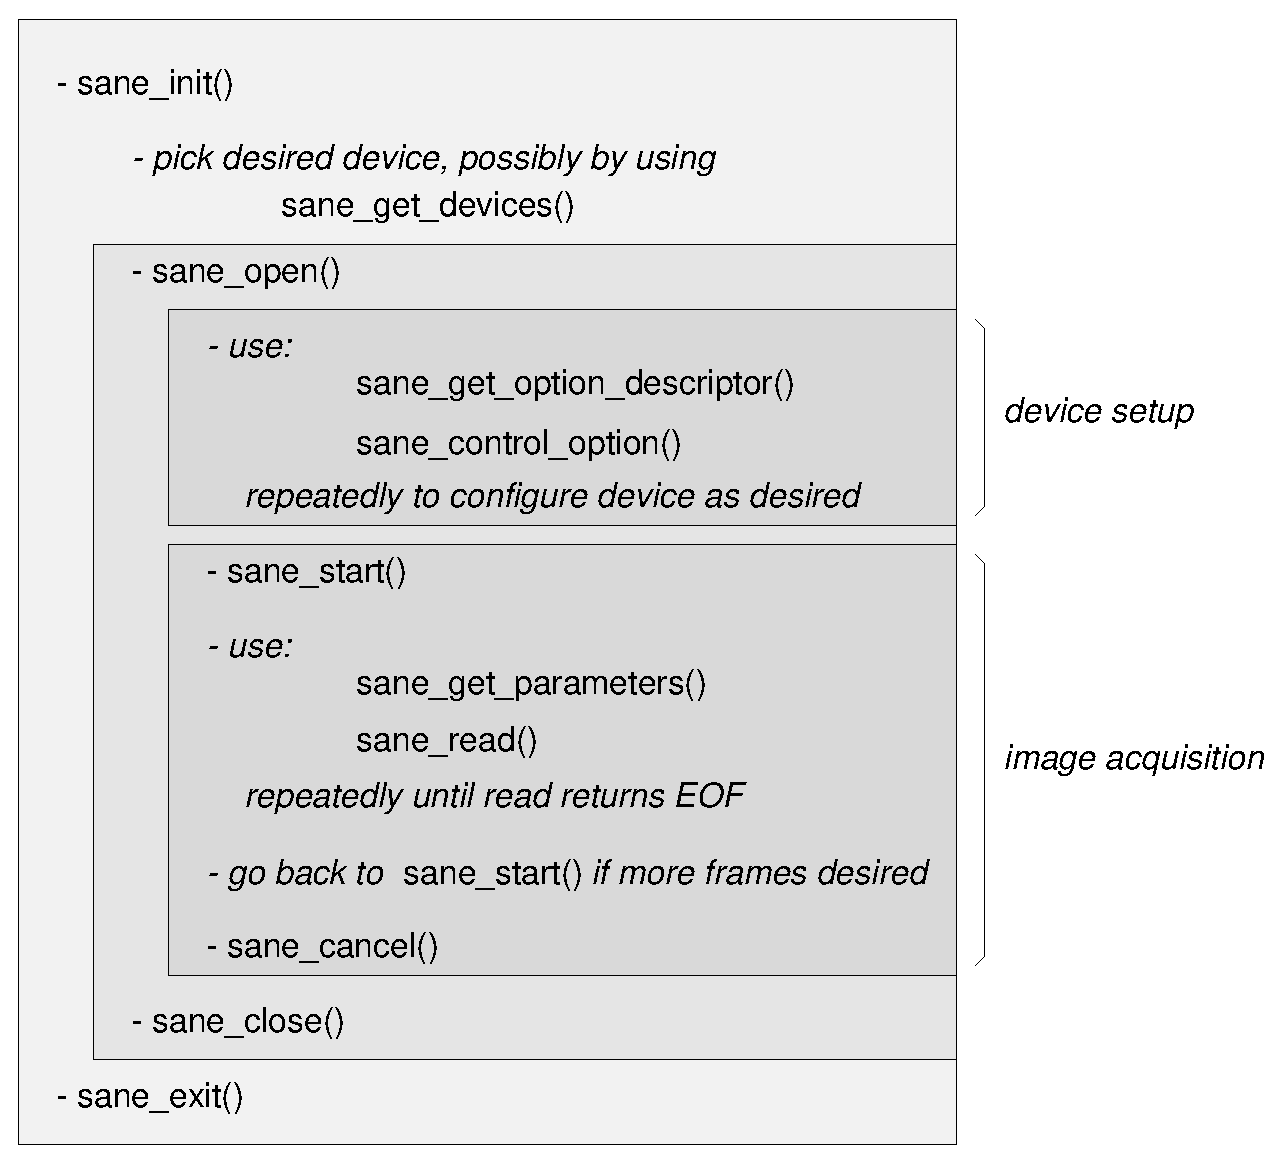
\psfig{file=figs/flow.eps,height=0.5\textheight}
    \caption{Code flow}
    \label{fig:flow}
  \end{center}
\end{figure}

Function \code{sane\_get\_devices()} can be called any time after
\code{sane\_init()} has been called.  It returns the list of the
devices that are known at the time of the call.  This list may change
over time since some devices may be turned on or off or a remote host
may boot or shutdown between different calls.  It should be noted that
this operation may be relatively slow since it requires contacting all
configured devices (some of which may be on remote hosts).  A frontend
may therefore want to provide the ability for a user to directly
select a desired device without requiring a call to this function.

Once a device has been chosen, it is opened using a call to
\code{sane\_open()}.  Multiple devices can be open at any given time.
A SANE backend must not impose artificial constraints on how many
devices can be open at any given time.

An opened device can be setup through the corresponding device handle
using functions \code{sane\_get\_opt\-ion\_desc\-riptor()} and
\code{sane\_control\_option()}.  While setting up a device, obtaining
option descriptors and setting and reading of option values can be
mixed freely.  It is typical for a frontend to read out all available
options at the beginning and then build a dialog (either graphical or
a command-line oriented option list) that allows to control the
available options.  It should be noted that the number of options is
fixed for a given handle.  However, as options are set, other options
may become active or inactive.  Thus, after setting an option, it
maybe necessary to re-read some or all option descriptors.  While
setting up the device, it is also admissible to call
\code{sane\_get\_parameters()} to get an estimate of what the image
parameters will look like once image acquisition begins.

The device handle can be put in blocking or non-blocking mode by a
call to \code{sane\_set\_io\_mode()}.  Devices are required to support
blocking mode (which is the default mode), but support for
non-blocking I/O is strongly encouraged for operating systems such as
UNIX.

After the device is setup properly, image acquisition can be started
by a call to \code{sane\_start()}.  The backend calculates the exact
image parameters at this point.  So future calls to
\code{sane\_get\_parameters()} will return the exact values, rather
than estimates.  Whether the physical image acquisition starts at this
point or during the first call to \code{sane\_read()} is unspecified
by the SANE API.  If non-blocking I/O and/or a select-style interface
is desired, the frontend may attempt to call
\code{sane\_set\_io\_mode()} and/or \code{sane\_get\_select\_fd()} at
this point.  Either of these functions may fail if the backend does
not support the requested operation.

Image data is collected by repeatedly calling \code{sane\_read()}.
Eventually, this function will return an end-of-file status
(\code{SANE\_STATUS\_EOF}).  This indicates the end of the current
frame.  If the frontend expects additional frames (e.g., the
individual channels in of a red/green/blue image or multiple images),
it can call \code{sane\_start()} again.  Once all desired frames have
been acquired, function \code{sane\_cancel()} must be called.  This
operation can also be called at any other time to cancel a pending
operation.  Note that \code{sane\_cancel()} must be called even if the
last read operation returned \code{SANE\_STATUS\_EOF}.

When done using the device, the handle should be closed by a call to
\code{sane\_close()}.  Finally, before exiting the application,
function \code{sane\_exit()} must be called.  It is important not to
forget to call this function since otherwise some resources (e.g.,
temporary files or locks) may remain unclaimed.


\section{Well-Known Options}\index{well-known options}

While most backend options are completely self-describing, there are a
cases where a user interface might want to special-case the handling
of certain options.  For example, the scan area is typically defined
by four options that specify the top-left and bottom-right corners of
the area.  With a graphical user interface, it would be tedious to
force the user to type in these four numbers.  Instead, most such
interfaces will want to present to the user a preview (low-resolution
scan) of the scanner surface and let the user pick the scan area by
dragging a rectangle into the desired position.  For this reason, the
SANE API specifies a small number of option names that have
well-defined meanings.

\subsection{Option Number Count}\index{option count}

Option number 0 has an empty string as its name.  The value of this
option is of type \code{SANE\_TYPE\_INT} and it specifies the total
number of options available for a given device (the count includes
option number 0).  This means that there are two ways of counting the
number of options available: a frontend can either cycle through all
option numbers starting at one until
\code{sane\_get\_option\_descriptor()} returns \code{NULL}, or a
frontend can directly read out the value of option number 0.

\subsection{Scan Resolution Option}\index{scan resolution}\index{resolution option}

Option \code{resolution} is used to select the resolution at which an
image should be acquired.  The type of this option is either
\code{SANE\_TYPE\_INT} or \code{SANE\_TYPE\_FIXED}.  The unit is
\code{SANE\_UNIT\_DPI} (dots/inch).

This option is not mandatory, but if a backend does support it, it
must implement it in a manner consistent with the above definition.

\subsection{Preview Mode Option}\index{preview mode}

The boolean option \code{preview} is used by a frontend to inform the
backend when image acquisition should be optimized for speed, rather
than quality (``preview mode'').  When set to \code{SANE\_TRUE},
preview mode is in effect, when set to \code{SANE\_FALSE} image
acquisition should proceed in normal quality mode.  The setting of
this option \emph{must not\/} affect any other option.  That is, as
far as the other options are concerned, the preview mode is completely
side effect free.  A backend can assume that the frontend will take
care of appropriately setting the scan resolution for preview mode
(through option \code{resolution}).  A backend is free to override the
\code{resolution} value with its own choice for preview mode, but it
is advised to leave this choice to the frontend wherever possible.

This option is not mandatory, but if a backend does support it, it
must implement it in a manner consistent with the above definition.

\subsection{Scan Area Options}\index{scan area options}

The four most important well-known options are the ones that define
the scan area.  The scan area is defined by two points (x/y coordinate
pairs) that specify the top-left and the bottom-right corners.  This
is illustrated in Figure~\ref{fig:area}.  Note that the origin of the
coordinate system is at the top-left corner of the scan surface as
seen by the sensor (which typically is a mirror image of the scan
surface seen by the user).  For this reason, the top-left corner is
the corner for which the abscissa and ordinate values are
simultaneously the {\em smallest} and the bottom-right corner is the
corner for which the abscissa and ordinate values are simulatenously
the {\em largest}.  If this coordinate system is not natural for a
given device, it is the job of the backend to perform the necessary
conversions.
\begin{figure}[tbp]
  \begin{center}
    \leavevmode
    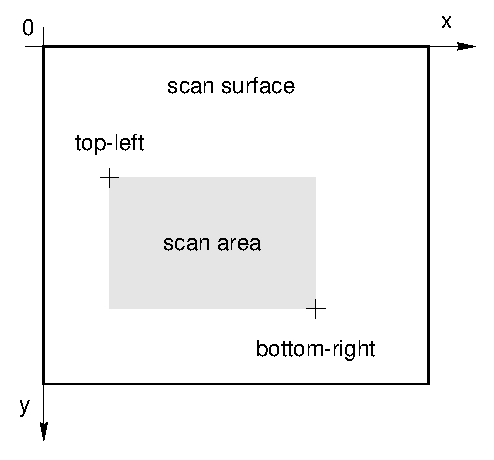
\psfig{file=figs/area.eps,height=0.3\textheight}
    \caption{Scan area options}
    \label{fig:area}
  \end{center}
\end{figure}

The names of the four options that define the scan area are given in
the table below:
\begin{center}
\begin{tabular}{ll}
{\bf Name} & {\bf Description} \\
\code{\defn{tl-x}} & Top-left $x$ coordinate value \\
\code{\defn{tl-y}} & Top-left $y$ coordinate value \\
\code{\defn{br-x}} & Bottom-right $x$ coordinate value \\
\code{\defn{br-y}} & Bottom-right $y$ coordinate value \\
\end{tabular}
\end{center}
There are several rules that should be followed by front and backends
regarding these options:
\begin{itemize}

\item Backends must attach a unit of either pixels
  (\code{SANE\_UNIT\_PIXEL}) or millimeters (\code{SANE\_UNIT\_MM}) to
  these options.  The unit of all four options must be identical.

\item Whenever meaningful, a backend should attach a range or a
  word-list constraint to these options.

\item A frontend can determine the size of the scan surface by first
  checking that the options have range constraints associated.  If a
  range or word-list constraints exist, the frontend can take the
  minimum and maximum values of one of the x and y option
  range-constraints to determine the scan surface size.

\item A frontend must work properly with any or all of these options
  missing.
  
\end{itemize}

\chapter{Network Protocol}\label{chap:net}

The SANE interface has been designed to facilitate network access to
image acquisition devices.  In particular, most SANE implementations
are expected to support a network backend (net client) and a
corresponding network daemon (net server) that allows accessing image
acquisition devices through a network connection.  Network access is
useful in several situations:
\begin{itemize}

\item To provide controlled access to resources that are inaccessible
  to a regular user.  For example, a user may want to access a device
  on a host where she has no account on.  With the network protocol,
  it is possible to allow certain users to access scanners without
  giving them full access to the system.

  Controlling access through the network daemon can be useful even in
  the local case: for example, certain backends may require root
  privileges to access a device.  Rather than installing each frontend
  as setuid-root, a system administrator could instead install the
  SANE network daemon as setuid-root.  This enables regular users to
  access the privileged device through the SANE daemon (which,
  presumably, supports a more fine-grained access control mechanism
  than the simple setuid approach).  This has the added benefit that
  the system administrator only needs to trust the SANE daemon, not
  each and every frontend that may need access to the privileged
  device.

\item Network access provides a sense of ubiquity of the available
  image acquisition devices.  For example, in a local area network
  environment, this allows a user to log onto any machine and have
  convenient access to any resource available to any machine on the
  network (subject to permission constraints).

\item For devices that do not require physical access when used (e.g.,
  video cameras), network access allows a user to control and use
  these devices without being in physical proximity.  Indeed, if such
  devices are connected to the Internet, access from any place in the
  world is possible.

\end{itemize}

The network protocol described in this chapter has been design with
the following goals in mind:
\begin{enumerate}

\item Image transmission should be efficient (have low encoding
  overhead).

\item Accessing option descriptors on the client side must be
  efficient (since this is a very common operation).

\item Other operations, such as setting or inquiring the value of an
  option are less performance critical since they typically require
  explicit user action.

\item The network protocol should be simple and easy to implement on
  any host architecture and any programming language.

\end{enumerate}
The SANE protocol can be run across any transport protocol that
provides reliable data delivery.  While SANE does not specify a
specific transport protocol, it is expected that TCP/IP will be among
the most commonly used protocols.

\section{Data Type Encoding}

\subsection{Primitive Data Types}

The four primitive types of the SANE standard are encoded as follows:
\begin{description}

\item[\code{\defn{SANE\_Byte}}:] A byte is encoded as an 8 bit value.
  Since the transport protocol is assumed to be byte-orientd, the bit
  order is irrelevant.

\item[\code{\defn{SANE\_Word}}:] A word is encoded as 4 bytes (32
  bits).  The bytes are ordered from most-significant to
  least-significant byte (big-endian byte-order).

\item[\code{\defn{SANE\_Char}}:] A character is currently encoded as an 8-bit
  ISO LATIN-1 value.  An extension to support wider character sets (16 or 32
  bits) is planned for the future, but not supported at this point.

\item[\code{\defn{SANE\_String}}:] A string pointer is encoded as a
  \code{SANE\_Char} array.  The trailing NUL byte is considered part
  of the array and a \code{NULL} pointer is encoded as a zero-length
  array.
  
\item[\code{\defn{SANE\_Handle}}:] A handle is encoded like a word.
  The network backend needs to take care of converting these integer
  values to the opaque pointer values that are presented to the user
  of the network backend.  Similarly, the SANE daemon needs to take
  care of converting the opaque pointer values it receives from its
  backends into 32-bit integers suitable for use for network encoding.

\item[{\em\defn{enumeration types}}:] Enumeration types are encoded
  like words.

\end{description}

\subsection{Type Constructors}

Closely following the type constructors of the C language, the SANE network
protocol supports the following four constructors:
\begin{description}

\item[{\em\defn{pointer}}:] A pointer is encoded by a word that indicates
  whether the pointer is a NULL-pointer which is then followed by the
  value that the pointer points to (in the case of a non-NULL pointer;
  in the case of a NULL pointer, no bytes are encoded for the pointer
  value).

\item[{\em\defn{array}}:] An array is encoded by a word that indicates
  the length of the array followed by the values of the elements in
  the array.  The length may be zero in which case no bytes are
  encoded for the element values.

\item[{\em\defn{structure}}:] A structure is encoded by simply encoding the
  structure members in the order in which they appear in the
  corresponding C type declaration.

\item[{\em\defn{union}}:] A union must always be accompanied by a tag
  value that indicates which of the union members is the currently the
  active one.  For this reason, the union itself is encoded simply by
  encoding the value of the currently active member.

\end{description}

Note that for type constructors, the pointer, element, or member
values themselves may have a constructed type.  Thus, the above rules
should be applied recursively until a sequence of primitive types has
been found.

Also SANE had no need for encoding of circular structures.  This
greatly simplifies the network protocol.

\section{Remote Procedure Call Requests}

The SANE network protocol is a client/server-style remote procedure
call (RPC) protocol.  This means that all activity is initiated by the
client side (the network backend)---a server is restricted to
answering request by the client.

\subsection{\code{\defn{SANE\_NET\_INIT}}}

This RPC establishes a connection to a particular SANE network daemon.
It must be the first call in a SANE network session.  The parameter
and reply arguments for this call are shown in the table below:
\begin{center}
\begin{tabular}{ll}
  {\bf request:} & {\bf reply:} \\
  \code{SANE\_Word version\_code} & \code{SANE\_Word status} \\
  \code{SANE\_String user\_name}   & \code{SANE\_Word version\_code} \\
\end{tabular}
\end{center}
The \code{version\_code} argument in the request is the SANE
version-code of the network backend that is contacting the network
daemon (see Section~\ref{sec:saneversioncode}).  The
``build-revision'' in the version code is used to hold the network
protocol version.  The SANE network daemon receiving such a request
must make sure that the network protocol version corresponds to a
supported version since otherwise the encoding of the network stream
may be incompatible (even though the SANE interface itself may be
compatible).  The \code{user\_name} argument is the name of the user
on whose behalf this call is being performed.  If the network backend
cannot determine a user-name, it passes a \code{NULL} pointer for this
argument.  No trust should be placed in the authenticity of this
user-name.  The intent of this string is to provide more convenience
to the user.  E.g., it could be used as the default-user name in
subsequent authentication calls.

In the reply, \code{status} indicates the completion status.  If the
value is anything other than \code{SANE\_STA\-TUS\_SUCCESS}, the
remainder of the reply has undefined values.\footnote{The sane network
  daemon should be careful not to leak information in the undefined
  portion of the reply.} The \code{version\_code} argument returns the
SANE version-code that the network daemon supports.  See the comments
in the previous paragraph on the meaning of the build-revision in this
version code.

\subsection{\code{\defn{SANE\_NET\_GET\_DEVICES}}}

This RPC is used to obtain the list of devices accessible by the SANE
daemon.
\begin{center}
\begin{tabular}{ll}
  {\bf request:} & {\bf reply:} \\
  \code{void} & \code{SANE\_Word status} \\
              & \code{SANE\_Device ***device\_list} \\
\end{tabular}
\end{center}
There are no arguments in the request for this call.

In the reply, \code{status} indicates the completion status.  If the
value is anything other than \code{SANE\_STA\-TUS\_SUCCESS}, the
remainder of the reply has undefined values.  The \code{device\_list}
argument is a pointer to a \code{NULL}-terminated array of
\code{SANE\_Device} pointers.

\subsection{\code{\defn{SANE\_NET\_OPEN}}}

This RPC is used to open a connection to a remote SANE device.
\begin{center}
\begin{tabular}{ll}
  {\bf request:} & {\bf reply:} \\
  \code{SANE\_String device\_name} & \code{SANE\_Word status} \\
                                   & \code{SANE\_Word handle} \\
                                   & \code{SANE\_String resource} \\
\end{tabular}
\end{center}
The \code{device\_name} argument specifies the name of the device to
open.

In the reply, \code{status} indicates the completion status.  If the
value is anything other than \code{SANE\_STA\-TUS\_SUCCESS}, the
remainder of the reply has undefined values.  The \code{handle}
argument specifies the device handle that uniquely identifies the
connection.  The \code{resource} argument is used to request
authentication.  If it has a non-\code{NULL} value, the network
backend should authenticate the specified resource and then retry this
operation (see Section~\ref{sec:authorization} for details on how to
authorize a resource).

\subsection{\code{\defn{SANE\_NET\_CLOSE}}}

This RPC is used to close a connection to a remote SANE device.
\begin{center}
\begin{tabular}{ll}
  {\bf request:} & {\bf reply:} \\
  \code{SANE\_Word handle} & \code{SANE\_Word dummy} \\
\end{tabular}
\end{center}
The \code{handle} argument identifies the connection that should be
closed.

In the reply, the \code{dummy} argument is unused.  Its purpose is to
ensure proper synchronization (without it, a net client would not be
able to determine when the RPC has completed).

\subsection{\code{\defn{SANE\_NET\_GET\_OPTION\_DESCRIPTORS}}}

This RPC is used to obtain {\em all\/} the option descriptors for a
remote SANE device.
\begin{center}
\begin{tabular}{ll}
  {\bf request:} & {\bf reply:} \\
  \code{SANE\_Word handle} & \code{Option\_Descriptor\_Array odesc} \\
\end{tabular}
\end{center}
The \code{handle} argument identifies the remote device whose option
descriptors should be obtained.

In the reply, the \code{odesc} argument is used to return the array of
option descriptors.  The option descriptor array has the following
structure:
\begin{quote}\index{Option\_Descriptor\_Array}
\begin{verbatim}
struct Option_Descriptor_Array
  {
    SANE_Word num_options;
    SANE_Option_Descriptor **desc;
  };
\end{verbatim}
\end{quote}


\subsection{\code{\defn{SANE\_NET\_CONTROL\_OPTION}}}

This RPC is used to control (inquire, set, or set to automatic) a
specific option of a remote SANE device.
\begin{center}
\begin{tabular}{ll}
  {\bf request:} & {\bf reply:} \\
  \code{SANE\_Word handle}      & \code{SANE\_Status status} \\
  \code{SANE\_Word option}      & \code{SANE\_Word info} \\
  \code{SANE\_Word action}      & \code{SANE\_Word value\_type} \\
  \code{SANE\_Word value\_type} & \code{SANE\_Word value\_size} \\
  \code{SANE\_Word value\_size} & \code{void *value} \\
  \code{void *value}            & \code{SANE\_String *resource} \\
\end{tabular}
\end{center}
The \code{handle} argument identifies the remote device whose option
should be controlled.  Argument \code{option} is the number (index) of
the option that should be controlled.  Argument \code{action}
specifies what action should be taken (get, set, or set automatic).
Argument \code{value\_type} specifies the type of the option value
(must be one of \code{SANE\_TYPE\_BOOL}, \code{SANE\_TYPE\_INT},
\code{SANE\_TYPE\_FIXED}, \code{SANE\_TYPE\_STR\-ING},
\code{SANE\_TYPE\_BUTTON}).  Argument \code{value\_size} specifies
the size of the option value in number of bytes (see
Section~\ref{sec:valuesize} for the precise meaning of this value).
Finally, argument \code{value} is a pointer to the option value.  It
must be a writeable area that is at least \code{value\_size} bytes
large. (Note that this area must be writable even if the action is to
set the option value.  This is because the backend may not be able to
set the exact option value, in which case the option value is used to
return the next best value that the backend has chosen.)

In the reply, argument \code{resource} is set to the name of the
resource that must be authorized before this call can be retried.  If
this value is non-\code{NULL}, all other arguments have undefined
values (see Section~\ref{sec:authorization} for details on how to
authorize a resource).  Argument \code{status} indicates the
completion status.  If the value is anything other than
\code{SANE\_STA\-TUS\_SUCCESS}, the remainder of the reply has undefined
values.  The \code{info} argument returns the information on how well
the backend was able to satisfy the request.  For details, see the
description of the corresponding argument in
Section~\ref{sec:control}.  Arguments \code{value\_type} and
\code{value\_size} have the same values as the arguments by the same
name in corresponding request.  The values are repeated here to ensure
that both the request and the reply are self-contained (i.e., they can
be encoded and decoded independently).  Argument \code{value} is holds
the value of the option that has become effective as a result of this
RPC.


\subsection{\code{\defn{SANE\_NET\_GET\_PARAMETERS}}}

This RPC is used to obtain the scan parameters of a remote SANE
device.
\begin{center}
\begin{tabular}{ll}
  {\bf request:} & {\bf reply:} \\
  \code{SANE\_Word handle} & \code{SANE\_Status status} \\
                           & \code{SANE\_Parameters params} \\
\end{tabular}
\end{center}
The \code{handle} argument identifies the connection to the remote
device whose scan parameters should be returned.

In the reply, \code{status} indicates the completion status.  If the
value is anything other than \code{SANE\_STA\-TUS\_SUC\-CESS}, the
remainder of the reply has undefined values.  The argument
\code{params} is used to return the scan parameters.

\subsection{\code{\defn{SANE\_NET\_START}}}

This RPC is used to start image acquisition (scanning).
\begin{center}
\begin{tabular}{ll}
  {\bf request:} & {\bf reply:} \\
  \code{SANE\_Word handle} & \code{SANE\_Status status} \\
                           & \code{SANE\_Word port} \\
                           & \code{SANE\_Word byte\_order} \\
                           & \code{SANE\_String resource} \\
\end{tabular}
\end{center}
The \code{handle} argument identifies the connection to the remote
device from which the image should be acquired.

In the reply, argument \code{resource} is set to the name of the
resource that must be authorized before this call can be retried.  If
this value is non-\code{NULL}, all other arguments have undefined
values (see Section~\ref{sec:authorization} for details on how to
authorize a resource).  Argument, \code{status} indicates the
completion status.  If the value is anything other than
\code{SANE\_STA\-TUS\_SUCCESS}, the remainder of the reply has
undefined values.  The argument \code{port} returns the port number
from which the image data will be available.  To read the image data,
a network client must connect to the remote host at the indicated port
number.  Through this port, the image data is transmitted as a
sequence of data records.  Each record starts with the data length in
bytes.  The data length is transmitted as a sequence of four bytes.
These bytes should be interpreted as an unsigned integer in big-endian
format.  The four length bytes are followed by the number of data
bytes indicated by the length.  Except for byte-order, the data is in
the same format as defined for \code{sane\_read()}.  Since some
records may contain no data at all, a length value of zero is
perfectly valid.  The special length value of \code{0xffffffff} is
used to indicate the end of the data stream.  That is, after receiving
a record length of \code{0xffffffff}, the network client should close
the data connection and stop reading data.

Argument \code{byte\_order} specifies the byte-order of the image
data.  A value of 0x1234 indicates little-endian format, a value of
0x4321 indicates big-endian format.  All other values are presently
undefined and reserved for future enhancements of this protocol.  The
intent is that a network server sends data in its own byte-order and
the client is responsible for adjusting the byte-order, if necessary.
This approach causes no unnecessary overheads in the case where the
server and client byte-order match and puts the extra burden on the
client side when there is a byte-order mismatch.  Putting the burden
on the client-side improves the scalability properties of this
protocol.

\subsection{\code{\defn{SANE\_NET\_CANCEL}}}

This RPC is used to cancel the current operation of a remote SANE
device.
\begin{center}
\begin{tabular}{ll}
  {\bf request:} & {\bf reply:} \\
  \code{SANE\_Word handle} & \code{SANE\_Word dummy} \\
\end{tabular}
\end{center}
The \code{handle} argument identifies the connection whose operation
should be cancelled.

In the reply, the \code{dummy} argument is unused.  Its purpose is to
ensure proper synchronization (without it, a net client would not be
able to determine when the RPC has completed).

\subsection{\code{\defn{SANE\_NET\_AUTHORIZE}}}\label{sec:authorization}
\index{network authorization}

This RPC is used to pass authorization data from the net client to the
net server.
\begin{center}
\begin{tabular}{ll}
  {\bf request:} & {\bf reply:} \\
  \code{SANE\_String resource} & \code{SANE\_Word dummy} \\
  \code{SANE\_String username} & \\
  \code{SANE\_String password} & \\
\end{tabular}
\end{center}
The \code{resource} argument specifies the name of the resource to be
authorized.  This argument should be set to the string returned in the
\code{resource} argument of the RPC reply that required this
authorization call.  The \code{username} and \code{password} are the
name of the user that is accessing the resource and the password for
the specified resource/user pair.

Since the password is not encrypted during network transmission, it is
recommended to use the following extension:

If the server adds the string `\code{\$MD5\$}' to the resource-name followed
by a random string not longer then 128 bytes, the client may answer with the
MD5 digest of the concatenation of the password and the random string. To
differentiate between the MD5 digest and a strange password the client prepends
the MD5 digest with the string `\code{\$MD5\$}'.

In the reply, \code{dummy} is completely unused.  Note that there is
no direct failure indication.  This is unnecessary since a net client
will retry the RPC that resulted in the authorization request until
that call succeeds (or until the request is cancelled). The RPC that resulted
in the authorization request continues after the reply from the client and may
fail with \code{SANE\_STATUS\_ACCESS\_DENIED}.


\subsection{\code{\defn{SANE\_NET\_EXIT}}}

This RPC is used to disconnect a net client from a net server.  There
are no request or reply arguments in this call.  As a result of this
call, the connection between the client and the server that was
established by the \code{SANE\_NET\_INIT} call will be closed.

% Local Variables: 
% mode: latex
% TeX-master: "sane.tex"
% End: 


\chapter{Contact Information}\label{chap:contact}

The SANE standard is discussed and evolved via a mailing list.
Anybody with email access to the Internet can automatically join and
leave the discussion group by sending mail to the following address.
\begin{quote}\index{mailing list}
\begin{verbatim}
sane-devel-request@lists.alioth.debian.org
\end{verbatim}
\end{quote}
To subscribe, send a mail with the body ``\verb|subscribe sane-devel|'' to the
above address.

A complete list of commands supported can be obtained by sending a
mail with a subject of ``\code{help}'' to the above address.  The
mailing list is archived and available through the SANE home page at
URL:
\begin{quote}
\url{http://www.sane-project.org/}
\end{quote}

\newpage
\documentclass[11pt,DVIps]{report}

\usepackage{times,epsfig,changebar,html}

\setlength{\parindent}{0pt}
\setlength{\parskip}{1.5ex plus 0.5ex minus 0.5ex}
\setlength{\textwidth}{6.5in}
\setlength{\textheight}{8.5in}
\setlength{\marginparwidth}{0pt}
\setlength{\oddsidemargin}{0pt}
\setlength{\evensidemargin}{0pt}
\setlength{\marginparsep}{0pt}
\addtolength{\topmargin}{-0.75in}

\title{\huge SANE Standard Version 1.02}
\author{}
\date{February 19, 2002} 

\makeindex

\begin{document}

\newcommand{\filename}[1]{{\tt #1}}
\newcommand{\code}[1]{{\tt #1}}
\newcommand{\var}[1]{{\it #1}}
\newcommand{\defn}[1]{#1\index{#1}}

\begin{latexonly}
  \setcounter{changebargrey}{0}   % black change bars
\end{latexonly}

\maketitle
\tableofcontents
\listoffigures
\listoftables


\chapter{Preface}

The SANE standard is being developed by a group of free-software
developers.  The process is open to the public and comments as well as
suggestions for improvements are welcome.  Information on how to join
the SANE development process can be found in Chapter
\ref{chap:contact}.

The SANE standard is intended to streamline software development by
providing a standard application programming interface to access
raster scanner hardware.  This should reduce the number of different
driver implementations, thereby reducing the need for reimplementing
similar code.


\section{About This Document}

This document is intended for developers who are creating either an
application that requires access to raster scanner hardware and for
developers who are implementing a SANE driver.  It does not cover
specific implementations of SANE components.  Its sole purpose is to
describe and define the SANE application interface that will enable
any application on any platform to interoperate with any SANE backend
for that platform.

The remainder of this document is organized as follows.
Chapter~\ref{chap:intro} provides introductional material.
Chapter~\ref{chap:environ} presents the environment SANE is designed
for.  Chapter~\ref{chap:api} details the SANE Application Programmer
Interface.  Chapter~\ref{chap:net} specifies the network protocol that
can be used to implement the SANE API in a network transparent
fashion.  Finally, Chapter~\ref{chap:contact} gives information on how
to join the SANE development process.

\subsection{Typographic Conventions}

Changes since the last revision of this document are highlighted
like this:

% \begin{changebar}
%   Paragraphs that changed since the last revision of the documention
%   are marked like this paragraph.
% \end{changebar}

\chapter{Introduction}\label{chap:intro}

SANE is an application programming interface (API) that provides
standardized access to any raster image scanner hardware.  The
standardized interface allows to write just one driver for each
scanner device instead of one driver for each scanner and application.
The reduction in the number of required drivers provides significant
savings in development time.  More importantly, SANE raises the level
at which applications can work.  As such, it will enable applications
that were previously unheard of in the UNIX world.  While SANE is
primarily targeted at a UNIX environment, the standard has been
carefully designed to make it possible to implement the API on
virtually any hardware or operating system.

SANE is an acronym for ``Scanner Access Now Easy.''  Also, the hope is
that SANE is sane in the sense that it will allow easy implementation
of the API while accommodating all features required by today's
scanner hardware and applications.  Specifically, SANE should be broad
enough to accommodate devices such as scanners, digital still and
video cameras, as well as virtual devices like image file filters.

\section{Terminology}

An application that uses the SANE interface is called a SANE {\em
  frontend}.  A driver that implements the SANE interface is called a
SANE {\em backend}.  A {\em meta backend\/} provides some means to
manage one or more other backends.


\chapter{The SANE Environment}\label{chap:environ}

SANE is defined as a C-callable library interface.  Accessing a raster
scanner device typically consists of two phases: first, various
controls of the scanner need to be setup or queried.  In the second
phase, one or more images are acquired.

Since the device controls are widely different from device to device,
SANE provides a generic interface that makes it easy for a frontend to
give a user access to all controls without having to understand each
and every device control.  The design principle used here is to
abstract each device control into a SANE {\em option\/}.  An option is
a self-describing name/value pair.  For example, the brightness
control of a camera might be represented by an option called
\code{brightness} whose value is an integer in the range from 0 to
255.

With self-describing options, a backend need not be concerned with
{\em presentation\/} issues: the backend simply provides a list of
options that describe all the controls available in the device.
Similarly, there are benefits to the frontend: it need not be
concerned with the {\em meaning\/} of each option.  It simply provides
means to present and alter the options defined by the backend.


\section{Attaching to a SANE backend}

The process through which a SANE frontend connects to a backend is
platform dependent.  Several possibilities exist:
\begin{itemize}

\item {\bf Static linking:} A SANE backend may be linked directly into
  a frontend.  While the simplest method of attaching to a backend, it
  is somewhat limited in functionality since the available devices is
  limited to the ones for which support has been linked in when the
  frontend was built.  But even so static linking can be quite useful,
  particularly when combined with a backend that can access scanners
  via a network.  Also, it is possible to support multiple backends
  simultaneously by implementing a meta backend that manages several
  backends that have been compiled in such a manner that they export
  unique function names.  For example, a backend called \code{be}
  would normally export a function called \code{sane\_read()}.  If
  each backend would provide such a function, static linking would
  fail due to multiple conflicting definitions of the same symbol.
  This can be resolved by having backend \code{be} include a
  header file that has lines of the form:
  \begin{quote}
\begin{verbatim}
#define sane_read be_sane_read
\end{verbatim}
  \end{quote}
  With definitions of this kind, backend \code{be} will export
  function name \code{be\_sane\_read()}.  Thus, all backends will
  export unique names.  As long as a meta backend knows about these
  names, it is possible to combine several backends at link time and
  select and use them dynamically at runtime.

\item {\bf Dynamic linking:} A simpler yet more powerful way to
  support multiple backends is to exploit dynamic linking on platforms
  that support it.  In this case, a frontend is linked against a
  shared library that implements any SANE backend.  Since each
  dynamically linked backend exports the same set of global symbols
  (all starting with the prefix \code{sane\_}), the dynamic library
  that gets loaded at runtime does not necessarily have to be the same
  one as one the frontend got linked against.  In other words, it is
  possible to switch the backend by installing the appropriate backend
  dynamic library.

  More importantly, dynamic linking makes it easy to implement a meta
  backend that loads other backends {\em on demand}.  This is a
  powerful mechanism since it allows adding new backends merely by
  installing a shared library and updating a configuration file.

\item {\bf Network connection:} Arguably the ultimate way to attach to
  a scanner is by using the network to connect to a backend on a
  remote machine.  This makes it possible to scan images from any host
  in the universe, as long as there is a network connection to that
  host and provided the user is permitted to access that scanner.

\end{itemize}

\begin{figure}[htbp]
  \begin{center}
    \leavevmode
    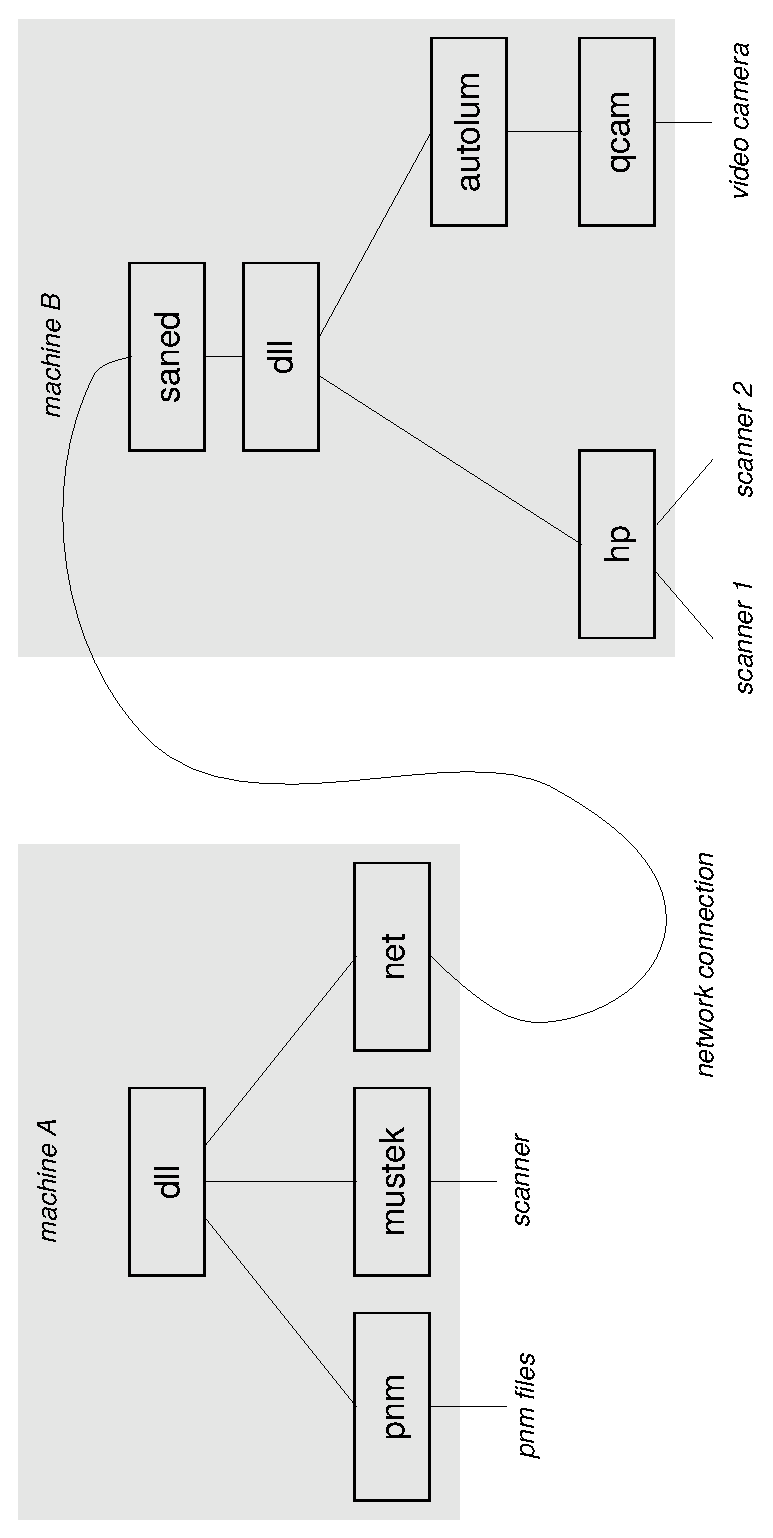
\psfig{file=figs/hierarchy.eps,angle=270,width=\textwidth}
    \caption{Example SANE Hiearchy}
    \label{fig:hierarchy}
  \end{center}
\end{figure}

The above discussion lists just a few ways for frontends to attach to
a backend.  It is of course possible to combine these solutions to
provide an entire hierarchy of SANE backends.  Such a hierarchy is
depicted in Figure~\ref{fig:hierarchy}.  The figure shows that machine
A uses a dynamic-linking based meta backend called \code{dll} to
access the backends called \code{pnm}, \code{mustek}, and \code{net}.
The first two are real backends, whereas the last one is a meta
backend that provides network transparent access to remote scanners.
In the figure, machine B provides non-local access to its scanners
through the SANE frontend called \code{saned}.  The \code{saned} in
turn has access to the \code{hp} and \code{autolum} backends through
another instance of the \code{dll} backend.  The \code{autolum} meta
backend is used to automatically adjust the luminance (brightness) of
the image data acquired by the camera backend called \code{qcam}.

Note that a meta backend really is both a frontend and a backend at
the same time.  It is a frontend from the viewpoint of the backends
that it manages and a backend from the viewpoint of the frontends that
access it.  The name ``meta backend'' was chosen primarily because the
SANE standard describes the interface from the viewpoint of a (real)
frontend.


\section{Image Data Format}\label{sec:imageformat}\index{image data format}

Arguably the most important aspect of an image acquisition system is
how images are represented.  The SANE approach is to define a simple
yet powerful representation that is sufficient for vast majority of
applications and devices.  While the representation is simple, the
interface has been defined carefully to allow extending it in the
future without breaking backwards compatibility.  Thus, it will be
possible to accommodate future applications or devices that were not
anticipated at the time this standard was created.

A SANE image is a rectangular area.  The rectangular area is
subdivided into a number of rows and columns.  At the intersection of
each row and column is a quadratic pixel.  A pixel consists of one or
more sample values.  Each sample value represents one channel (e.g.,
the red channel).  Each sample value has a certain bit depth.  The bit
depth is fixed for the entire image and can be as small as one bit.
Valid bit depths are 1, 8, or 16 bits per sample.  If a device's
natural bit depth is something else, it is up to the driver to scale
the sample values appropriately (e.g., a 4 bit sample could be scaled
by a factor of four to represent a sample value of depth 8).

\subsection{Image Transmission}

The SANE API transmits an image as a sequence of frames.  Each frame
covers the same rectangular area as the entire image, but may contain
only a subset of the channels in the final image.  For example, a
red/green/blue image could either be transmitted as a single frame
that contains the sample values for all three channels or it could be
transmitted as a sequence of three frames: the first frame containing
the red channel, the second the green channel, and the third the blue
channel.

Conceptually, each frame is transmitted a byte at a time.  Each byte
may contain 8 sample values (for an image bit depth of 1), one full
sample value (for an image bit depth of 8), or a partial sample value
(for an image bit depth of 16 or bigger).  In the latter case, the
bytes of each sample value are transmitted in the machine's native
byte order.
\begin{quote}
  \begin{center}
    {\bf Backend Implementation Note}
  \end{center}
  A network-based meta backend will have to ensure that the byte order
  in image data is adjusted appropriately if necessary.  For example,
  when the meta backend attaches to the server proxy, the proxy may
  inform the backend of the server's byte order.  The backend can then
  apply the adjustment if necessary.  In essence, this implements a
  ``receiver-makes-right'' approach.
\end{quote}

\begin{figure}[htbp]
  \begin{center}
    \leavevmode
    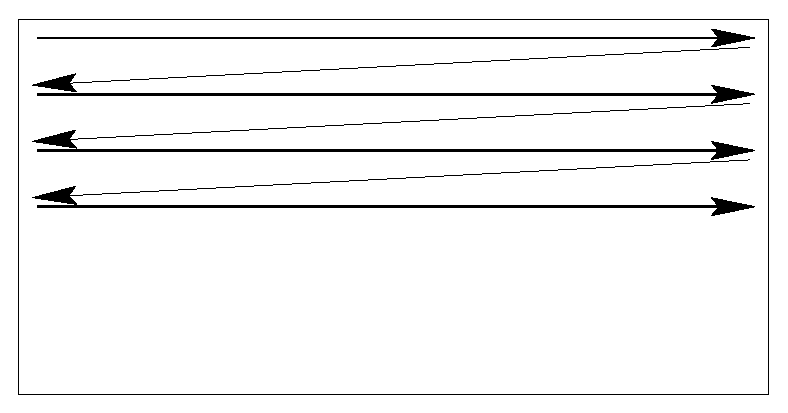
\psfig{file=figs/xfer.eps,width=0.5\textwidth}
    \caption{Transfer order of image data bytes}
    \label{fig:xfer}
  \end{center}
\end{figure}

The order in which the sample values in a frame are transmitted is
illustrated in Figure~\ref{fig:xfer}.  As can be seen, the values are
transmitted row by row and each row is transmitted from left-most to
right-most column.  The left-to-right, top-to-bottom transmission
order applies when the image is viewed in its normal orientation (as
it would be displayed on a screen, for example).

If a frame contains multiple channels, then the channels are
transmitted in an interleaved fashion.  Figure~\ref{fig:pixels}
illustrates this for the case where a frame contains a complete
red/green/blue image with a bit-depth of 8.  For a bit depth of 1,
each byte contains 8 sample values of a {\em single\/} channel.  In
other words, a bit depth 1 frame is transmitted in a byte interleaved
fashion.

\begin{figure}[htbp]
  \begin{center}
    \leavevmode
    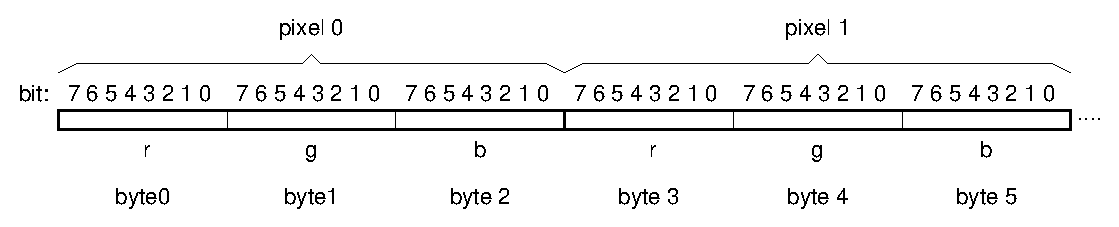
\psfig{file=figs/image-data.eps,width=0.8\textwidth}
    \caption{Bit and byte order or image data}
    \label{fig:pixels}
  \end{center}
\end{figure}

When transmitting an image frame by frame, the frontend needs to know
what part of the image a frame represents (and how many frames it
should expect).  For that purpose, the SANE API tags every frame with
a type.  This version of the SANE standard supports the following
frame types:
\begin{quote}
\begin{description}

\item[\code{\defn{SANE\_FRAME\_GRAY}}:] The frame contains a single
  channel of data that represents sample values from a spectral band
  that covers the human visual range.  The image consists of this
  frame only.

\item[\code{\defn{SANE\_FRAME\_RGB}}:] The frame contains three
  channels of data that represent sample values from the red, green,
  and blue spectral bands.  The sample values are interleaved in the
  order red, green, and blue.  The image consists of this frame only.

\item[\code{\defn{SANE\_FRAME\_RED}}:] The frame contains one channel
  of data that represents sample values from the red spectral band.
  The complete image consists of three frames:
  \code{SANE\_\-FRA\-ME\_RED}, \code{SANE\_FRAME\_GREEN}, and
  \code{SANE\_FRAME\_BLUE}.  The order in which the frames are
  transmitted chosen by the backend.

\item[\code{\defn{SANE\_FRAME\_GREEN}}:] The frame contains one
  channel of data that represents sample values from the green
  spectral band.  The complete image consists of three frames:
  \code{SANE\_\-FRA\-ME\_RED}, \code{SANE\_FRAME\_GREEN}, and
  \code{SANE\_FRAME\_BLUE}.  The order in which the frames are
  transmitted chosen by the backend.

\item[\code{\defn{SANE\_FRAME\_BLUE}}:] The frame contains one channel
  of data that represents sample values from the blue spectral band.
  The complete image consists of three frames:
  \code{SANE\_\-FRA\-ME\_RED}, \code{SANE\_FRAME\_GREEN}, and
  \code{SANE\_FRAME\_BLUE}.  The order in which the frames are
  transmitted chosen by the backend.

\end{description}
\end{quote}

In frames of type SANE\_FRAME\_GRAY, when the bit depth is 1 there are
only two sample values possible, 1 represents minimum intensity
(black) and 0 represents maximum intensity (white).  For all other bit
depth and frame type combinations, a sample value of 0 represents
minimum intensity and larger values represent increasing intensity.


\chapter{The SANE Application Programmer Interface (API)}\label{chap:api}

This Section defines version 1 of the SANE application
programmer interface (API).  Any SANE frontend must depend on the
interface defined in this section only.  Converseley, any SANE backend
must implement its functionality in accordance with this
specification.  The interface as documented here is declared as a C
callable interface in a file called \filename{sane/sane.h}.  This file should
normally be included via a C pre-processor directive of the form:
\begin{verbatim}
  #include <sane/sane.h>
\end{verbatim}


\section{Version Control}

The SANE standard is expected to evolve over time.  Whenever a change
to the SANE standard is made that may render an existing frontend or
backend incompatible with the new standard, the major version number
must be increased.  Thus, any frontend/backend pair is compatible
provided the major version number of the SANE standard they implement
is the same.  A frontend may implement backwards compatiblity by
allowing major numbers that are smaller than the expected major number
(provided the frontend really can cope with the older version).  In
contrast, a backend always provides support for one and only one
version of the standard.  If a specific application does require that
two different versions of the same backend are accessible at the same
time, it is possible to do so by installing the two versions under
different names.

SANE version control also includes a minor version number and a build
revision.  While control of these numbers remains with the implementor
of a backend, the recommended use is as follows.  The minor version is
incremented with each official release of a backend.  The build
revision is increased with each build of a backend.

The SANE API provides the following five macros to manage version
numbers.
\begin{quote}
  \begin{description}
  \item[\code{\defn{SANE\_CURRENT\_MAJOR}}:] The value of this macro is the
    number of the SANE standard that the interface implements.

  \item[\code{\defn{SANE\_VERSION\_CODE}(\var{maj},\var{min},\var{bld})}:]
    \label{sec:saneversioncode}
    This macro can be used to build a monotonically increasing version
    code.  A SANE version code consists of the SANE standard major
    version number (\var{maj}), the minor version number \var{min},
    and the build revision of a backend (\var{bld}).  The major and
    minor version numbers must be in the range 0\ldots255 and the
    build revision must be in the range 0\ldots65535.

    Version codes are monotonic in the sense that it is possible to
    apply relational operators (e.g., equality or less-than test)
    directly on the version code rather than individually on the three
    components of the version code.

    Note that the major version number alone determines whether a
    frontend/backend pair is compatible.  The minor version and the
    build revision are used for informational and bug-fixing purposes
    only.
  
  \item[\code{\defn{SANE\_VERSION\_MAJOR}(\var{vc})}:] This macro returns the
    major version number component of the version code passed in
    argument \var{vc}.
  \item[\code{SANE\_VERSION\_MINOR(\var{vc})}:] This macro returns the
    minor version number component of the version code passed in
    argument \var{vc}.
  \item[\code{SANE\_VERSION\_BUILD(\var{vc})}:] This macro returns the
    build revision component of the version code passed in argument
    \var{vc}.
  \end{description}
\end{quote}


\section{Data Types}

\subsection{Base Types}

The SANE standard is based on just two SANE-specific base types: the
SANE byte and word.
\begin{quote}
  \code{typedef \var{some-scalar-type\/} \defn{SANE\_Byte};} \\
  \code{typedef \var{some-scalar-type\/} \defn{SANE\_Word};}
\end{quote}
\verb|SANE_Byte| must correspond to some scalar C type that is capable
of holding values in the range 0 to 255.  \verb|SANE_Word| must be
capable of holding any of the following:
\begin{itemize}
  \item the truth values \verb|SANE_FALSE| and \verb|SANE_TRUE|
  \item signed integers in the range $-2^{31}\ldots2^{31}-1$
  \item fixed point values in the range $-32768\ldots32767.9999$ with
    a resolution of $1/65536$
  \item 32 bits (for bit sets)
\end{itemize}
Note that the SANE standard does not define what C type
\verb|SANE_Byte| and \verb|SANE_Word| map to.  For example, on some
platforms, the latter may map to \verb|long int| whereas on others it
may map to \verb|int|.  A portable SANE frontend or backend must
therefore not depend on a particular mapping.

\subsection{Boolean Type}

\code{\defn{SANE\_Bool}} is used for variables that can take one of
the two truth values \code{\defn{SANE\_FALSE}} and
\code{\defn{SANE\_TRUE}}.  The former value is defined to be 0,
whereas the latter is 1.\footnote{This is different from ANSI C where
  any non-zero integer value represents logical TRUE.} The C
declarations for this type are given below.
\begin{quote}
\begin{verbatim}
#define SANE_FALSE      0
#define SANE_TRUE       1
typedef SANE_Word SANE_Bool;
\end{verbatim}
\end{quote}
Note that \verb|SANE_Bool| is simply an alias of \verb|SANE_Word|.  It
is therefore always legal to use the latter type in place of the
former.  However, for clarity, it is recommended to use
\verb|SANE_Bool| whenever a given variable or formal argument has a
fixed interpretation as a boolean object.

\subsection{Integer Type}

\code{\defn{SANE\_Int}} is used for variables that can take integer
values in the range $-2^{32}$ to $2^{31}-1$.  Its C declaration is
given below.
\begin{quote}
\begin{verbatim}
typedef SANE_Word SANE_Int;
\end{verbatim}
\end{quote}
Note that \verb|SANE_Int| is simply an alias of \verb|SANE_Word|.  It
is therefore always legal to use the latter type in place of the
former.  However, for clarity, it is recommended to use
\verb|SANE_Int| whenever a given variable or formal argument has a
fixed interpretation as an integer object.


\subsection{Fixed-point Type}

\code{\defn{SANE\_Fixed}} is used for variables that can take fixed
point values in the range $-32768$ to $32767.9999$ with a resolution
of $1/65535$.  The C declarations relating to this type are given
below.
\begin{quote}
\begin{verbatim}
#define SANE_FIXED_SCALE_SHIFT  16
typedef SANE_Word SANE_Fixed;
\end{verbatim}
\end{quote}
The macro \code{\defn{SANE\_FIXED\_SCALE\_SHIFT}} gives the location
of the fixed binary point.  This standard defines that value to be 16,
which yields a resolution of $1/65536$.

Note that \verb|SANE_Fixed| is simply an alias of \verb|SANE_Word|.
It is therefore always legal to use the latter type in place of the
former.  However, for clarity, it is recommended to use
\verb|SANE_Fixed| whenever a given variable or formal argument has a
fixed interpretation as a fixed-point object.

For convenience, SANE also defines two macros that convert fixed-point
values to and from C double floating point values.
\begin{quote}
  \begin{description}

  \item[\code{\defn{SANE\_FIX}(\var{d})}:] Returns the largest SANE
    fixed-point value that is smaller than the double value \var{d}.
    No range checking is performed.  If the value of \var{d} is out of
    range, the result is undefined.

  \item[\code{\defn{SANE\_UNFIX}(\var{w})}:] Returns the nearest
    double machine number that corresponds to fixed-point value
    \var{w}.

  \end{description}
\end{quote}
SANE does {\em not\/} require that the following two expressions hold
true (even if the values of \var{w} and \var{d} are in range):
\begin{quote}
\begin{verbatim}
SANE_UNFIX(SANE_FIX(d)) == d
SANE_FIX(SANE_UNFIX(w)) == w
\end{verbatim}
\end{quote}
In other words, conversion between fixed and double values may be
lossy.  It is therefore recommended to avoid repeated conversions
between the two representations.


\subsection{Text}

\subsubsection{Character Type}

Type \code{\defn{SANE\_Char}} represents a single text character or
symbol.  At present, this type maps directly to the underlying C
\verb|char| type (typically one byte).  The encoding for such
characters is currently fixed as ISO LATIN-1.  Future versions of this
standard may map this type to a wider type and allow multi-byte
encodings to support internationalization.  As a result of this, care
should be taken to avoid the assumption that
\verb|sizeof(SANE_Char)==sizeof(char)|.
\begin{quote}
\begin{verbatim}
typedef char SANE_Char;
\end{verbatim}
\end{quote}

\subsubsection{String Type}

Type \code{\defn{SANE\_String}} represents a text string as a sequence
of C \verb|char| values.  The end of the sequence is indicated by a
\verb|'\0'| (\defn{NUL}) character.  
\begin{quote}
\begin{verbatim}
typedef SANE_Char *SANE_String;
typedef const SANE_Char *SANE_String_Const;
\end{verbatim}
\end{quote}
The type \code{\defn{SANE\_String\_Const}} is provided by SANE to
enable declaring strings whose contents is unchangable.  Note that in
ANSI C, the declaration
\begin{quote}
\begin{verbatim}
const SANE_String str;
\end{verbatim}
\end{quote}
declares a string pointer that is constant (not a string pointer that
points to a constant value).


\subsection{Scanner Handle Type}

Access to a scanner is provided through an opaque type called
\code{\defn{SANE\_Handle}}.  The C declaration of this type is given
below.
\begin{quote}
\begin{verbatim}
typedef void *SANE_Handle;
\end{verbatim}
\end{quote}
While this type is declared to be a void pointer, an application must
not attempt to interpret the value of a \verb|SANE_Handle|.  In
particular, SANE does not require that a value of this type is a legal
pointer value.


\subsection{Status Type}

Most SANE operations return a value of type \code{\defn{SANE\_Status}}
to indicate whether the completion status of the operation.  If an
operation completes successfully, \verb|SANE_STATUS_GOOD| is returned.
In case of an error, a value is returned that indicates the nature of
the problem.  The complete list of available status codes is listed in
Table \ref{tab:status}.  It is recommended to use function
\code{sane\_strstatus()} to convert status codes into a legible
string.

\begin{table}[htbp]
  \begin{center}
    \begin{tabular}{|l|r|l|}
      \hline
      \multicolumn{1}{|c|}{\bf Symbol} & \multicolumn{1}{c|}{\bf Code} &
      \multicolumn{1}{c|}{\bf Description} \\
      \hline\hline
\code{\defn{SANE\_STATUS\_GOOD}}
        &  0 & Operation completed succesfully. \\
\code{\defn{SANE\_STATUS\_UNSUPPORTED}}
        &  1 & Operation is not supported. \\
\code{\defn{SANE\_STATUS\_CANCELLED}}
        &  2 & Operation was cancelled. \\
\code{\defn{SANE\_STATUS\_DEVICE\_BUSY}}
        &  3 & Device is busy---retry later. \\
\code{\defn{SANE\_STATUS\_INVAL}}
        &  4 & Data or argument is invalid. \\
\code{\defn{SANE\_STATUS\_EOF}}
        &  5 & No more data available (end-of-file). \\
\code{\defn{SANE\_STATUS\_JAMMED}}
        &  6 & Document feeder jammed. \\
\code{\defn{SANE\_STATUS\_NO\_DOCS}}
        &  7 & Document feeder out of documents. \\
\code{\defn{SANE\_STATUS\_COVER\_OPEN}}
        &  8 & Scanner cover is open. \\
\code{\defn{SANE\_STATUS\_IO\_ERROR}}
        &  9 & Error during device I/O. \\
\code{\defn{SANE\_STATUS\_NO\_MEM}}
        & 10 & Out of memory. \\
\code{\defn{SANE\_STATUS\_ACCESS\_DENIED}}
        & 11 & Access to resource has been denied. \\
      \hline
    \end{tabular}
    \caption{Status Codes}\label{tab:status}
  \end{center}
\end{table}


\subsection{Device Descriptor Type}

Each SANE device is represented by a structure of type
\code{\defn{SANE\_Device}}.  The C declaration of this type is given
below.
\begin{quote}
\begin{verbatim}
typedef struct
  {
    SANE_String_Const name;
    SANE_String_Const vendor;
    SANE_String_Const model;
    SANE_String_Const type;
  }
SANE_Device;
\end{verbatim}
\end{quote}
\index{device-name}
The structure provides the unique name of the scanner in member
\code{name}.  It is this unique name that should be passed in a call
to \code{sane\_open()}.  The format of this name is completely up to
the backend.  The only constraints are that the name is unique among
all devices supported by the backend and that the name is a legal SANE
text string.  To simplify presentation of unique names, their length
should not be excessive.  It is {\em recommended\/} that backends keep
unique names below 32 characters in length.  However, applications
{\em must\/} be able to cope with arbitrary length unique names.

The remaining members in the device structure provide additional
information on the device corresponding to the unique name.
Specifically, members \code{vendor}, \code{model}, and \code{type} are
single-line strings that give information on the vendor
(manufacturer), model, and the type of the device.  For consistency's
sake, the following strings should be used when appropriate (the lists
will be expanded as need arises):

\begin{table}[htbp]
  \begin{center}
    \leavevmode
    \hspace{\fill}
    \begin{tabular}[t]{|ll|}
      \hline
      \multicolumn{2}{|c|}{\bf \defn{Vendor Strings}} \\
      \hline\hline
      \code{AGFA}            & \code{Microtek} \\
      \code{Abaton}          & \code{Minolta} \\
      \code{Acer}            & \code{Mustek} \\
      \code{Apple}           & \code{NEC} \\
      \code{Artec}           & \code{Nikon} \\
      \code{Avision}         & \code{Plustek} \\
      \code{CANON}           & \code{Polaroid} \\
      \code{Connectix}       & \code{Ricoh} \\
      \code{Epson}           & \code{Sharp} \\
      \code{Fujitsu}         & \code{Siemens} \\
      \code{Hewlett-Packard} & \code{Tamarack} \\
      \code{IBM}             & \code{UMAX} \\
      \code{Kodak}           & \code{Noname} \\
      \code{Logitech}        & \\
      \hline
    \end{tabular}
    \hspace{\fill}
    \begin{tabular}[t]{|l|}
      \hline
      \multicolumn{1}{|c|}{\bf \defn{Type Strings}} \\
      \hline\hline
      \code{film scanner} \\
      \code{flatbed scanner} \\
      \code{frame grabber} \\
      \code{handheld scanner} \\
      \code{sheetfed scanner} \\
      \code{still camera} \\
      \code{video camera} \\
      \code{virtual device} \\
      \hline
    \end{tabular}
    \hspace{\fill}
    \caption{Predefined Device Information Strings}
    \label{tab:devinfo}
  \end{center}
\end{table}
Note that vendor string \code{Noname} can be used for virtual devices
that have no physical vendor associated.  Also, there are no
predefined model name strings since those are vendor specific and
therefore completely under control of the respective backends.


\subsection{Option Descriptor Type}\label{sec:odesc}

Option descriptors are at the same time the most intricate and
powerful type in the SANE standard.  Options are used to control
virtually all aspects of device operation.  Much of the power of the
SANE API stems from the fact that most device controls are completely
described by their respective option descriptor.  Thus, a frontend can
control a scanner abstractly, without requiring knowledge as to what
the purpose of any given option is.  Conversely, a scanner can
describe its controls without requiring knowledge of how the frontend
operates.  The C declaration of the
\code{\defn{SANE\_Option\_Descriptor}} type is given below.
\begin{quote}
\begin{verbatim}
typedef struct
  {
    SANE_String_Const name;
    SANE_String_Const title;
    SANE_String_Const desc;
    SANE_Value_Type type;
    SANE_Unit unit;
    SANE_Int size;
    SANE_Int cap;
    SANE_Constraint_Type constraint_type;
    union
      {
        const SANE_String_Const *string_list;
        const SANE_Word *word_list;
        const SANE_Range *range;
      }
    constraint;
  }
SANE_Option_Descriptor;
\end{verbatim}
\end{quote}

\subsubsection{Option Name}

Member \code{name} is a string that uniquely identifies the option.
The name must be unique for a given device (i.e., the option names
across different backends or devices need not be unique).  The option
name must consist of lower-case ASCII letters (\code{a}--\code{z}),
digits (\code{0}--\code{9}), or the dash character (\code{-}) only.
The first character must be a lower-case ASCII character (i.e., not a
digit or a dash).

\subsubsection{Option Title}

Member \code{title} is a single-line string that can be used by the
frontend as a title string.  This should typically be a short (one or
two-word) string that is chosen based on the function of the option.

\subsubsection{Option Description}

Member \code{desc} is a (potentially very) long string that can be
used as a help text to describe the option.  It is the responsibility
of the frontend to break the string into managable-length lines.
Newline characters in this string should be interpreted as paragraph
breaks.

\subsubsection{Option Value Type}

Member \code{type} specifies the type of the option value.  The
possible values for type \code{\defn{SANE\_Value\_Type}} are described
in Table \ref{tab:valuetype}.

\begin{table}[htbp]
  \begin{center}
    \leavevmode
    \begin{tabular}{|l|l|p{0.6\textwidth}|}
\hline
\multicolumn{1}{|c|}{\bf Symbol} &
\multicolumn{1}{c|}{\bf Code} &
\multicolumn{1}{c|}{\bf Description} \\
\hline\hline

\code{\defn{SANE\_TYPE\_BOOL}} & 0 & Option value is of type
  \verb|SANE_Bool|. \\ 

\code{\defn{SANE\_TYPE\_INT}} & 1 & Option value is of type
  \verb|SANE_Int|. \\ 

\code{\defn{SANE\_TYPE\_FIXED}}&2 & Option value is of type
  \verb|SANE_Fixed|. \\ 

\code{\defn{SANE\_TYPE\_STRING}}&3 & Option value is of type
  \verb|SANE_String|. \\ 

\code{\defn{SANE\_TYPE\_BUTTON}} & 4 & An option of this type has no value.
Instead, setting an option of this type has an option-specific
side-effect.  For example, a button-typed option could be used by a
backend to provide a means to select default values or to the tell an
automatic document feeder to advance to the next sheet of paper. \\ 

\code{\defn{SANE\_TYPE\_GROUP}} & 5 & An option of this type has no value.
This type is used to group logically related options.  A group option
is in effect up to the point where another group option is encountered
(or up to the end of the option list, if there are no other group
options).  For group options, only members \code{title} and
\code{type} are valid in the option descriptor. \\ 

  \hline
    \end{tabular}
    \caption{Option Value Types (\code{SANE\_Value\_Type})}
    \label{tab:valuetype}
  \end{center}
\end{table}

\subsubsection{Option Value Unit}

Member \code{unit} specifies what the physical unit of the option
value is.  The possible values for type \code{\defn{SANE\_U\-nit}} are
described in Table \ref{tab:units}.  Note that the specified unit is
what the SANE backend expects.  It is entirely up to a frontend as to
how these units a presented to the user.  For example, SANE expresses
all lengths in millimeters.  A frontend is generally expected to
provide appropriate conversion routines so that a user can express
quantities in a customary unit (e.g., inches or centimeters).

\begin{table}[htbp]
  \begin{center}
    \leavevmode
    \begin{tabular}{|l|l|l|}
\hline
\multicolumn{1}{|c|}{\bf Symbol} &
\multicolumn{1}{|c|}{\bf Code} &
\multicolumn{1}{|c|}{\bf Description} \\

\hline\hline

\code{\defn{SANE\_UNIT\_NONE}}   & 0 & Value is unit-less (e.g., page count).\\
\code{\defn{SANE\_UNIT\_PIXEL}}  & 1 & Value is in number of pixels. \\
\code{\defn{SANE\_UNIT\_BIT}}    & 2 & Value is in number of bits. \\
\code{\defn{SANE\_UNIT\_MM}}     & 3 & Value is in millimeters. \\
\code{\defn{SANE\_UNIT\_DPI}}    & 4 & Value is a resolution in dots/inch. \\
\code{\defn{SANE\_UNIT\_PERCENT}}& 5 & Value is a percentage. \\
\code{\defn{SANE\_UNIT\_MICROSECOND}}& 6 & Value is time in $\mu$-seconds. \\

\hline
    \end{tabular}
    \caption{Physical Units (\code{SANE\_Unit})}
    \label{tab:units}
  \end{center}
\end{table}

\subsubsection{Option Value Size}\label{sec:valuesize}

Member \code{size} specifies the size of the option value (in bytes).
This member has a slightly different interpretation depending on the
type of the option value:
\begin{quote}
  \begin{description}
  \item[\code{SANE\_TYPE\_STRING}:] The size is the maximum size of
    the string.  For the purpose of string size calcuations, the
    terminating \code{NUL} character is considered to be part of the
    string.  Note that the terminating \code{NUL} character must
    always be present in string option values.
  \item[\code{SANE\_TYPE\_INT}, \code{SANE\_TYPE\_FIXED}:] The size
    must be a positive integer multiple of the size of a
    \verb|SANE_Word|.  The option value is a vector of length
    \[ \code{size}/\code{sizeof(SANE\_Word)}. \]
  \item[\code{SANE\_TYPE\_BOOL}:] The size must be set to
    \code{sizeof(SANE\_Word)}.
  \item[\code{SANE\_TYPE\_BUTTON}, \code{SANE\_TYPE\_GROUP}:] The
    option size is ignored.
  \end{description}
\end{quote}

\subsubsection{Option Capabilities}

Member \code{cap} describes what capabilities the option posseses.
This is a bitset that is formed as the inclusive logical OR of the
capabilities described in Table \ref{tab:capabilities}.  The SANE API
provides the following to macros to test certain features of a given
capability bitset:
\begin{quote}
  \begin{description}

  \item[\code{\defn{SANE\_OPTION\_IS\_ACTIVE}(\var{cap})}:] This macro
    returns \code{SANE\_TRUE} if and only if the option with the
    capability set \var{cap} is currently active.

  \item[\code{\defn{SANE\_OPTION\_IS\_SETTABLE}(\var{cap})}:] This
    macro returns \code{SANE\_TRUE} if and only if the option with the
    capability set \var{cap} is software settable.
  \end{description}
\end{quote}

\begin{table}[htbp]
  \begin{center}
    \leavevmode
    \begin{tabular}{|l|r|p{0.59\textwidth}|}
\hline
\multicolumn{1}{|c|}{\bf Symbol} &
\multicolumn{1}{c|}{\bf Code} &
\multicolumn{1}{c|}{\bf Description} \\
\hline\hline

\code{\defn{SANE\_CAP\_SOFT\_SELECT}} & 1 & The option
  value can be set by a call to \code{sane\_con\-trol\_opt\-ion()}.\\ 

\code{\defn{SANE\_CAP\_HARD\_SELECT}} & 2 & The option value can be set by
  user-intervention (e.g., by flipping a switch).  The user-interface
  should prompt the user to execute the appropriate action to set such
  an option.  This capability is mutually exclusive with
  SANE\_CAP\_SOFT\_SELECT (either one of them can be set, but not both
  simultaneously).  \\ 

\code{\defn{SANE\_CAP\_SOFT\_DETECT}} & 4 & The option
  value can be detected by software.  If
  \code{SANE\_\-CAP\_\-SO\-FT\_SEL\-ECT} is set, this capability {\em must\/}
  be set.  If \code{SANE\_CAP\_HARD\_SELECT} is set, this capability
  may or may not be set.  If this capability is set but neither
  \code{SANE\_CAP\_SO\-FT\_SEL\-ECT} nor \code{SANE\_CAP\_HA\-RD\_SEL\-ECT}
  are, then there is no way to control the option.  That is, the
  option provides read-out of the current value only.  \\ 

\code{\defn{SANE\_CAP\_EMULATED}} & 8 & If set, this capability indicates
  that an option is not directly supported by the device and is
  instead emulated in the backend.  A sophisticated frontend may
  elect to use its own (presumably better) emulation in lieu of an emulated
  option. \\ 

\code{\defn{SANE\_CAP\_AUTOMATIC}} & 16 & If set, this capability indicates
  that the backend (or the device) is capable to picking a reasonable
  option value automatically.  For such options, it is possible to
  select automatic operation by calling \code{sane\_control\_option()}
  with an action value of \code{SANE\_ACTION\_SET\_AUTO}.  \\ 

\code{\defn{SANE\_CAP\_INACTIVE}} & 32 & If set, this capability indicates
  that the option is not currently active (e.g., because it's
  meaningful only if another option is set to some other value). \\ 

\code{\defn{SANE\_CAP\_ADVANCED}} & 64 &
  If set, this capability indicates that the option should be
  considered an ``advanced user option.''  A frontend typically
  displays such options in a less conspicuous way than regular options
  (e.g., a command line interface may list such options last or a
  graphical interface may make them available in a seperate ``advanced
  settings'' dialog). 
  \\

\hline
    \end{tabular}
    \caption{Option Capabilities}
    \label{tab:capabilities}
  \end{center}
\end{table}

\subsubsection{Option Value Constraints}

It is often useful to constrain the values that an option can take.
For example, constraints can be used by a frontend to determine how to
represent a given option.  Member \code{constraint\_type} indicates
what constraint is in effect for the option.  The constrained values
that are allowed for the option are described by one of the union
members of member \code{constraint}.  The possible values of type
\code{\defn{SANE\_Constraint\_Type}} and the interpretation of the
\code{constraint} union is described in Table~\ref{tab:constraints}.

\begin{table}[htbp]
  \begin{center}
    \leavevmode
    \begin{tabular}{|l|r|p{0.5\textwidth}|}
\hline
\multicolumn{1}{|c|}{\bf Symbol} &
\multicolumn{1}{|c|}{\bf Code} &
\multicolumn{1}{|c|}{\bf Description} \\

\hline\hline

\code{\defn{SANE\_CONSTRAINT\_NONE}} & 0 & The value is unconstrained.
  The option can take any of the values possible for the option's
  type. \\

  \code{\defn{SANE\_CONSTRAINT\_RANGE}} & 1 & This constraint is
  applicable to integer and fixed-point valued options only.  It
  constrains the option value to a possibly quantized range of
  numbers.  Option descriptor member \code{constraint.range} points to
  a range of the type \code{\defn{SANE\_Range}}.  This type is illustrated
  below:
  \begin{quote}
\begin{verbatim}
typedef struct
  {
    SANE_Word min;
    SANE_Word max;
    SANE_Word quant;
  }
SANE_Range;
\end{verbatim}
  \end{quote}
  All three members in this structure are interpreted according to the
  option value type (\verb|SANE_TYPE_INT| or \verb|SANE_TYPE_FIXED|).
  Members \code{min} and \code{max} specify the minimum and maximum
  values, respectively.  If member \code{quant} is non-zero, it
  specifies the quantization value.  If $l$ is the minimum value, $u$
  the maximum value and $q$ the (non-zero) quantization of a range,
  then the legal values are $v=k\cdot q+l$ for all non-negative
  integer values of $k$ such that $v<=u$.  \\ 

\code{\defn{SANE\_CONSTRAINT\_WORD\_LIST}} & 2 & This constraint is applicable
  to integer and fixed-point valued options only.  It constrains the
  option value to a list of numeric values.  Option descriptor member
  \code{constraint.word\_list} points to a list of words that
  enumerates the legal values.  The first element in that list is an
  integer (\verb|SANE_Int|) that specifies the length of the list (not
  counting the length itself).  The remaining elements in the list are
  interpreted according to the type of the option value
  (\verb|SANE_TYPE_INT| or \verb|SANE_TYPE_FIXED|). \\ 

\code{\defn{SANE\_CONSTRAINT\_STRING\_LIST}} & 3 & This constraint is
  applicable to string-valued options only.  It constrains the option
  value to a list of strings.  The option descriptor member
  \code{con\-strai\-nt.str\-ing\_list} points to a \code{NULL} terminated
  list of strings that enumerate the legal values for the option
  value.
\\\hline
    \end{tabular}
    \caption{Option Value Constraints}
    \label{tab:constraints}
  \end{center}
\end{table}


\section{Operations}

\subsection{\code{sane\_init}}

This function must be called before any other SANE function can be
called.  The behavior of a SANE backend is undefined if this function
is not called first.  The version code of the backend is returned in
the value pointed to by \code{version\_code}.  If that pointer is
\code{NULL}, no version code is returned. 
  Argument \code{authorize} is either a pointer to a function that is
  invoked when the backend requires authentication for a specific
  resource or \code{NULL} if the frontend does not support
  authentication.
\begin{quote}\index{sane\_init}
\begin{verbatim}
SANE_Status sane_init (SANE_Int * version_code,
                       SANE_Authorization_Callback authorize);
\end{verbatim}
\end{quote}

The authorization function may be called by a backend in response to
any of the following calls:
\begin{quote}
  \code{sane\_open}, \code{sane\_control\_option}, \code{sane\_start}
\end{quote}
If a backend was initialized without authorization function, then
authorization requests that cannot be handled by the backend itself
will fail automatically and the user may be prevented from accessing
protected resources.  Backends are encouraged to implement means of
authentication that do not require user assistance.  E.g., on a
multi-user system that authenticates users through a login process a
backend could automatically lookup the apporpriate password based on
resource- and user-name.

The authentication function type has the following declaration:
\begin{quote}\index{SANE\_Authorization\_Callback}
  \index{domain}\index{username}\index{password}
\begin{verbatim}
#define SANE_MAX_USERNAME_LEN   128
#define SANE_MAX_PASSWORD_LEN   128

typedef void (*SANE_Authorization_Callback)
    (SANE_String_Const resource,
     SANE_Char username[SANE_MAX_USERNAME_LEN],
     SANE_Char password[SANE_MAX_PASSWORD_LEN]);
\end{verbatim}
\end{quote}
Three arguments are passed to the authorization function:
\code{resource} is a string specifying the name of the resource that
requires authorization.  A frontend should use this string to build a
user-prompt requesting a username and a password.  The \code{username}
and \code{password} arguments are (pointers to) an array of
\code{SANE\_MAX\_USERNAME\_LEN} and \code{SANE\_MAX\_PASSWORD\_LEN}
characters, respectively.  The authorization call should place the
entered username and password in these arrays.  The returned strings
{\em must\/} be ASCII-NUL terminated.

\subsection{\code{sane\_exit}}

This function must be called to terminate use of a backend.  The
function will first close all device handles that still might be open
(it is recommended to close device handles explicitly through a call
to \code{sane\_clo\-se()}, but backends are required to release all
resources upon a call to this function).  After this function returns,
no function other than \code{sane\_init()} may be called (regardless
of the status value returned by \code{sane\_exit()}.  Neglecting to
call this function may result in some resources not being released
properly.
\begin{quote}\index{sane\_exit}
\begin{verbatim}
void sane_exit (void);
\end{verbatim}
\end{quote}


\subsection{\code{sane\_get\_devices}}

This function can be used to query the list of devices that are
available.  If the function executes successfully, it stores a pointer
to a \code{NULL} terminated array of pointers to \verb|SANE_Device|
structures in \code{*device\_list}.  The returned list is guaranteed
to remain unchanged and valid until (a) another call to this function
is performed or (b) a call to \code{sane\_exit()} is performed.  This
function can be called repeatedly to detect when new devices become
available.  If argument \code{local\_only} is true, only local devices
are returned (devices directly attached to the machine that SANE is
running on).  If it is false, the device list includes all remote
devices that are accessible to the SANE library.
\begin{quote}\index{sane\_get\_devices}
\begin{verbatim}
SANE_Status sane_get_devices (const SANE_Device *** device_list,
                              SANE_Bool local_only);
\end{verbatim}
\end{quote}

This function may fail with \code{SANE\_STATUS\_NO\_MEM} if an
insufficient amount of memory is available.

\begin{quote}
  \begin{center}
    {\bf Backend Implementation Note}
  \end{center}
  SANE does not require that this function is called before a
  \code{sane\_open()} call is performed.  A device name may be
  specified explicitly by a user which would make it unnecessary and
  undesirable to call this function first.
\end{quote}


\subsection{\code{sane\_open}}

This function is used to establish a connection to a particular
device.  The name of the device to be opened is passed in argument
\code{name}.  If the call completes successfully, a handle for the
device is returned in \code{*h}.  As a special case, specifying a
zero-length string as the device requests opening the first available
device (if there is such a device).
\begin{quote}\index{sane\_open}
\begin{verbatim}
SANE_Status sane_open (SANE_String_Const name, SANE_Handle * h);
\end{verbatim}
\end{quote}

This function may fail with one of the following status codes.
\begin{quote}
\begin{description}
\item[\code{SANE\_STATUS\_DEVICE\_BUSY}:] The device is currently
  busy (in use by somebody else).
\item[\code{SANE\_STATUS\_INVAL}:] The device name is not valid.
\item[\code{SANE\_STATUS\_IO\_ERROR}:] An error occured while
  communicating with the device.
\item[\code{SANE\_STATUS\_NO\_MEM}:] An insufficent amount of memory
  is available.
\item[\code{SANE\_STATUS\_ACCESS\_DENIED}:] Access to the device has
  been denied due to insufficient or invalid authentication.
\end{description}
\end{quote}


\subsection{\code{sane\_close}}

This function terminates the association between the device handle
passed in argument \code{h} and the device it represents.  If the
device is presently active, a call to \code{sane\_cancel()} is
performed first.  After this function returns, handle \code{h} must
not be used anymore.

\begin{quote}\index{sane\_close}
\begin{verbatim}
void sane_close (SANE_Handle h);
\end{verbatim}
\end{quote}

\subsection{\code{sane\_get\_option\_descriptor}}

This function is used to access option descriptors.  The function
returns the option descriptor for option number \code{n} of the device
represented by handle \code{h}.  Option number 0 is guaranteed to be a
valid option.  Its value is an integer that specifies the number of
options that are available for device handle \code{h} (the count
includes option 0).  If $n$ is not a valid option index, the function
returns \code{NULL}.  The returned option descriptor is guaranteed to
remain valid (and at the returned address) until the device is closed.

\begin{quote}\index{sane\_get\_option\_descriptor}
\begin{verbatim}
const SANE_Option_Descriptor *
    sane_get_option_descriptor (SANE_Handle h, SANE_Int n);
\end{verbatim}
\end{quote}

\subsection{\code{sane\_control\_option}}\label{sec:control}

This function is used to set or inquire the current value of option
number \code{n} of the device represented by handle \code{h}.  The
manner in which the option is controlled is specified by parameter
\code{a}.  The possible values of this parameter are described in more
detail below.  The value of the option is passed through argument
\code{v}.  It is a pointer to the memory that holds the option value.
The memory area pointed to by \code{v} must be big enough to hold the
entire option value (determined by member \code{size} in the
corresponding option descriptor).  The only exception to this rule is
that when setting the value of a string option, the string pointed to
by argument \code{v} may be shorter since the backend will stop
reading the option value upon encountering the first \code{NUL}
terminator in the string.  If argument \code{i} is not \code{NULL},
the value of \code{*i} will be set to provide details on how well the
request has been met.  The meaning of this argument is described in
more detail below.
\begin{quote}\index{sane\_control\_option}
\begin{verbatim}
SANE_Status sane_control_option (SANE_Handle h, SANE_Int n,
                                 SANE_Action a, void *v,
                                 SANE_Int * i);
\end{verbatim}
\end{quote}

The way the option is affected by a call to this function is
controlled by parameter \code{a} which is a value of type
\code{\defn{SANE\_Action}}.  The possible values and their meaning is
described in Table~\ref{tab:actions}.

\begin{table}[h]
  \begin{center}
    \leavevmode
    \begin{tabular}{|l|r|p{0.5\textwidth}|}
\hline
\multicolumn{1}{|c|}{\bf Symbol} &
\multicolumn{1}{|c|}{\bf Code} &
\multicolumn{1}{|c|}{\bf Description} \\

\hline\hline

\code{\defn{SANE\_ACTION\_GET\_VALUE}} & 0 & Get current option value. \\

\code{\defn{SANE\_ACTION\_SET\_VALUE}} & 1 & Set option value.  The
  option value passed through argument \code{v} may be modified by the
  backend if the value cannot be set exactly.  \\ 

\code{\defn{SANE\_ACTION\_SET\_AUTO}} & 2 & Turn on automatic mode.  Backend
  or device will automatically select an appropriate value.  This mode
  remains effective until overridden by an explicit set value request.
  The value of parameter \code{v} is completely ignored in this case and
  may be \code{NULL}.  \\

\hline
    \end{tabular}
    \caption{Action Values (\code{SANE\_Action})}
    \label{tab:actions}
  \end{center}
\end{table}

After setting a value via an action value of
\verb|SANE_ACTION_SET_VALUE|, additional information on how well the
request has been met is returned in \code{*i} (if \code{i} is
non-\code{NULL}).  The returned value is a bitset that may contain any
combination of the values described in Table~\ref{tab:info}.
\begin{table}[htbp]
  \begin{center}
    \leavevmode
    \begin{tabular}{|l|r|p{0.5\textwidth}|}
\hline
\multicolumn{1}{|c|}{\bf Symbol} &
\multicolumn{1}{|c|}{\bf Code} &
\multicolumn{1}{|c|}{\bf Description} \\

\hline\hline

\code{\defn{SANE\_INFO\_INEXACT}} & 1 & This value is returned when
  setting an option value resulted in a value being selected that does
  not exactly match the requested value.  For example, if a scanner
  can adjust the resolution in increments of 30dpi only, setting the
  resolution to 307dpi may result in an actual setting of 300dpi.
  When this happens, the bitset returned in \code{*i} has this member
  set.  In addition, the option value is modified to reflect the
  actual (rounded) value that was used by the backend.  Note that
  inexact values are admissible for strings as well.  A backend may
  choose to ``round'' a string to the closest matching legal string
  for a constrained string value. \\

  \code{\defn{SANE\_INFO\_RELOAD\_OPTIONS}} & 2 & The setting of an
  option may affect the value or availability of one or more {\em
    other\/} options.  When this happens, the SANE backend sets this
  member in \code{*i} to indicate that the application should reload
  all options.  This member may be set if and only if at least one
  option changed. \\

\code{\defn{SANE\_INFO\_RELOAD\_PARAMS}} & 4 & The setting of an option may
  affect the parameter values (see \code{sane\_get\_parameters()}).
  If setting an option affects the parameter values, this member will
  be set in \code{*i}.  Note that this member may be set even if the
  parameters did not actually change.  However, it is guaranteed that
  the parameters never change without this member being set. \\

\hline
    \end{tabular}
    \caption{Additional Information Returned When Setting an Option}
    \label{tab:info}
  \end{center}
\end{table}

This function may fail with one of the following status codes.
\begin{quote}
\begin{description}
\item[\code{SANE\_STATUS\_UNSUPPORTED}:] The operation is not
  supported for the specified handle and option number.
\item[\code{SANE\_STATUS\_INVAL}:] The option value is not valid.
\item[\code{SANE\_STATUS\_IO\_ERROR}:] An error occured while
  communicating with the device.
\item[\code{SANE\_STATUS\_NO\_MEM}:] An insufficent amount of memory
  is available.
\item[\code{SANE\_STATUS\_ACCESS\_DENIED}:] Access to the option has
  been denied due to insufficient or invalid authentication.
\end{description}
\end{quote}



\subsection{\code{sane\_get\_parameters}}

This function is used to obtain the current scan parameters.  The
returned parameters are guaranteed to be accurate between the time a
scan has been started (\code{sane\_start()} has been called) and the
completion of that request.  Outside of that window, the returned
values are best-effort estimates of what the parameters will be when
\code{sane\_start()} gets invoked.  Calling this function before a
scan has actually started allows, for example, to get an estimate of
how big the scanned image will be.  The parameters passed to this
function are the handle \code{h} of the device for which the
parameters should be obtained and a pointer \code{p} to a parameter
structure.  The parameter structure is described in more detail below.

\begin{quote}\index{sane\_get\_parameters}
\begin{verbatim}
SANE_Status sane_get_parameters (SANE_Handle h,
                                 SANE_Parameters * p);
\end{verbatim}
\end{quote}

The scan parameters are returned in a structure of type
\code{\defn{SANE\_Parameters}}.  The C declaration of this structure
is given below.
\begin{quote}
\begin{verbatim}
typedef struct
  {
    SANE_Frame format;
    SANE_Bool last_frame;
    SANE_Int lines;
    SANE_Int depth;
    SANE_Int pixels_per_line;
    SANE_Int bytes_per_line;
  }
SANE_Parameters;
\end{verbatim}
\end{quote}

Member \code{format} specifies the format of the next frame to be
returned.  The possible values for type \code{\defn{SANE\_Frame}} are
described in Table~\ref{tab:frameformat}.  The meaning of these
values is described in more detail in Section~\ref{sec:imageformat}.
\begin{table}[htbp]
  \begin{center}
    \leavevmode
    \begin{tabular}{|l|r|l|}
\hline
\multicolumn{1}{|c|}{\bf Symbol} &
\multicolumn{1}{|c|}{\bf Code} &
\multicolumn{1}{|c|}{\bf Description} \\

\hline\hline

\code{\defn{SANE\_FRAME\_GRAY}} & 0 & Band covering human visual range. \\
\code{\defn{SANE\_FRAME\_RGB}} & 1 & Pixel-interleaved red/green/blue bands. \\
\code{\defn{SANE\_FRAME\_RED}} & 2 & Red band of a red/green/blue image. \\
\code{\defn{SANE\_FRAME\_GREEN}} & 3 & Green band of a red/green/blue image. \\
\code{\defn{SANE\_FRAME\_BLUE}} & 4 & Blue band of a red/green/blue image. \\

\hline
    \end{tabular}
    \caption{Frame Format (\code{SANE\_Frame})}
    \label{tab:frameformat}
  \end{center}
\end{table}

Member \code{last\_frame} is set to \code{SANE\_TRUE} if and only if
the frame that is currently being acquired (or the frame that will be
acquired next if there is no current frame) is the last frame of a
multi frame image (e.g., the current frame is the blue component of a
red, green, blue image).

Member \code{lines} specifies how many scan lines the frame is
comprised of.  If this value is -1, the number of lines is not known a
priori and the frontend should call \code{sane\_read()} until it
returns a status of \code{SANE\_STATUS\_EOF}.

Member \code{bytes\_per\_line} specifies the number of bytes that
comprise one scan line.

Member \code{depth} specifies the number of bits per sample.

Member \code{pixels\_per\_line} specifies the number of pixels that
comprise one scan line.

Assume $B$ is the number of channels in the frame, then the bit depth
$d$ (as given by member \code{depth}) and the number of pixels per
line $n$ (as given by this member \code{pixels\_per\_line}) are
related to $c$, the number of bytes per line (as given by member
\code{bytes\_per\_line}) as follows:
\[
  c >= \left\{
  \begin{array}{ll}
    \lceil B\cdot n / 8\rceil & \mbox{if $d=1$}\\
    B\cdot n \cdot \lceil (d + 7)/8 \rceil & \mbox{if $d>1$}
  \end{array}
  \right.
\]
Note that the number of bytes per line can be larger than the minimum
value imposed by the right side of this equation.  A frontend must be
able to properly cope with such ``padded'' image formats.


\subsection{\code{sane\_start}}

This function initiates aquisition of an image from the device
represented by handle \code{h}.
\begin{quote}\index{sane\_start}
\begin{verbatim}
SANE_Status sane_start (SANE_Handle h);
\end{verbatim}
\end{quote}
This function may fail with one of the following status codes.
\begin{quote}
\begin{description}
\item[\code{SANE\_STATUS\_CANCELLED}:] The operation was cancelled through
  a call to \code{sane\_cancel}.
\item[\code{SANE\_STATUS\_DEVICE\_BUSY}:] The device is busy. The
  operation should be retried later.
\item[\code{SANE\_STATUS\_JAMMED}:] The document feeder is jammed.
\item[\code{SANE\_STATUS\_NO\_DOCS}:] The document feeder is out of
  documents.
\item[\code{SANE\_STATUS\_COVER\_OPEN}:] The scanner cover is open.
\item[\code{SANE\_STATUS\_IO\_ERROR}:] An error occurred while communicating
  with the device.
\item[\code{SANE\_STATUS\_NO\_MEM}:] An insufficent amount of memory
  is available.
\end{description}
\end{quote}


\subsection{\code{sane\_read}}

This function is used to read image data from the device represented
by handle \code{h}.  Argument \code{buf} is a pointer to a memory area
that is at least \code{maxlen} bytes long.  The number of bytes
returned is stored in \code{*len}.  A backend must set this to zero
when a status other than \code{SANE\_STA\-TUS\_GOOD} is returned.
When the call succeeds, the number of bytes returned can be anywhere in
the range from 0 to \code{maxlen} bytes.
\begin{quote}\index{sane\_read}
\begin{verbatim}
SANE_Status sane_read (SANE_Handle h, SANE_Byte * buf,
                       SANE_Int maxlen, SANE_Int * len);
\end{verbatim}
\end{quote}
If this function is called when no data is available, one of two
things may happen, depending on the I/O mode that is in effect for
handle \code{h}.
\begin{enumerate}
\item If the device is in blocking I/O mode (the default mode), the
  call blocks until at least one data byte is available (or until some
  error occurs).

\item If the device is in non-blocking I/O mode, the call returns
  immediately with status \code{SANE\_STA\-TUS\_GOOD} and with
  \code{*len} set to zero.
\end{enumerate}
The I/O mode of handle \code{h} can be set via a call to
\code{sane\_set\_io\_mode()}.

This function may fail with one of the following status codes.
\begin{quote}
\begin{description}
\item[\code{SANE\_STATUS\_CANCELLED}:] The operation was cancelled through
  a call to \code{sane\_cancel}.
\item[\code{SANE\_STATUS\_EOF}:] No more data is available for the
  current frame.
\item[\code{SANE\_STATUS\_JAMMED}:] The document feeder is jammed.
\item[\code{SANE\_STATUS\_NO\_DOCS}:] The document feeder is out of
  documents.
\item[\code{SANE\_STATUS\_COVER\_OPEN}:] The scanner cover is open.
\item[\code{SANE\_STATUS\_IO\_ERROR}:] An error occurred while communicating
  with the device.
\item[\code{SANE\_STATUS\_NO\_MEM}:] An insufficent amount of memory
  is available.
\item[\code{SANE\_STATUS\_ACCESS\_DENIED}:] Access to the device has
  been denied due to insufficient or invalid authentication.
\end{description}
\end{quote}


\subsection{\code{sane\_cancel}}

This function is used to immediately or as quickly as possible cancel
the currently pending operation of the device represented by handle
\code{h}.
\begin{quote}\index{sane\_cancel}
\begin{verbatim}
void sane_cancel (SANE_Handle h);
\end{verbatim}
\end{quote}
This function can be called at any time (as long as handle \code{h} is
a valid handle) but usually affects long-running operations only (such
as image is acquisition).  It is safe to call this function
asynchronously (e.g., from within a signal handler).  It is important
to note that completion of this operaton does {\em not\/} imply that
the currently pending operation has been cancelled.  It only
guarantees that cancellation has been {\em initiated}.  Cancellation
completes only when the cancelled call returns (typically with a
status value of \code{SANE\_STATUS\_CANCELLED}).  Since the SANE API
does not require any other operations to be re-entrant, this implies
that a frontend must {\em not\/} call any other operation until the
cancelled operation has returned.


\subsection{\code{sane\_set\_io\_mode}}

This function is used to set the I/O mode of handle \code{h}.  The I/O
mode can be either blocking or non-blocking.  If argument \code{m} is
\code{SANE\_TRUE}, the mode is set to non-blocking mode, otherwise
it's set to blocking mode.
\begin{quote}\index{sane\_set\_io\_mode}
\begin{verbatim}
SANE_Status sane_set_io_mode (SANE_Handle h, SANE_Bool m);
\end{verbatim}
\end{quote}
By default, newly opened handles operate in blocking mode.  A backend
may elect not to support non-blocking I/O mode.  In such a case the
status value \code{SANE\_STATUS\_UNSUPPORTED} is returned.  Blocking
I/O must be supported by all backends, so calling this function with
argument \code{m} set to \code{SANE\_FALSE} is guaranteed to complete
successfully.

This function may fail with one of the following status codes:
\begin{quote}
\begin{description}
\item[\code{SANE\_STATUS\_INVAL}:] No image acquisition is pending.
\item[\code{SANE\_STATUS\_UNSUPPORTED}:] The backend does not support
  this operation.
\end{description}
\end{quote}


\subsection{\code{sane\_get\_select\_fd}}

This function is used to obtain a (platform-specific) file-descriptor
for handle \code{h} that is readable if and only if image data is
available (i.e., when a call to \code{sane\_read()} will return at
least one byte of data).  If the call completes successfully, the
select file-descriptor is returned in \code{*fd}.
\begin{quote}\index{sane\_get\_select\_fd}
\begin{verbatim}
SANE_Status sane_get_select_fd (SANE_Handle h, SANE_Int *fd);
\end{verbatim}
\end{quote}
This function can be called only after a call to \code{sane\_start()}
has been performed and the returned file-descriptor is guaranteed to
remain valid for the duration of the current image acquisition (i.e.,
until \code{sane\_cancel()} or \code{sane\_start()} get called again
or until \code{sane\_read()} returns with status
\code{SANE\_STA\-TUS\_EOF}).  Indeed, a backend must guarantee to
close the returned select file descriptor at the point when the next
\code{sane\_read()} call would return \code{SANE\_STA\-TUS\_EOF}.
This is necessary to ensure the application can detect when this
condition occurs without actually having to call \code{sane\_read()}.

A backend may elect not to support this operation.  In such a case,
the function returns with status code
\code{SANE\_STATUS\_UNSUPPORTED}.

Note that the only operation supported by the returned file-descriptor
is a host operating-system dependent test whether the file-descriptor
is readable (e.g., this test can be implemented using \code{select()}
or \code{poll()} under UNIX).  If any other operation is performed on
the file descriptor, the behavior of the backend becomes
unpredictable.  Once the file-descriptor signals ``readable'' status,
it will remain in that state until a call to \code{sane\_read()} is
performed.  Since many input devices are very slow, support for this
operation is strongly encouraged as it permits an application to do
other work while image acquisition is in progress.

This function may fail with one of the following status codes:
\begin{quote}
\begin{description}
\item[\code{SANE\_STATUS\_INVAL}:] No image acquisition is pending.
\item[\code{SANE\_STATUS\_UNSUPPORTED}:] The backend does not support
  this operation.
\end{description}
\end{quote}


\subsection{\code{sane\_strstatus}}

This function can be used to translate a SANE status code into a
printable string.  The returned string is a single line of text that
forms a complete sentence, but without the trailing period
(full-stop).  The function is guaranteed to never return \code{NULL}.
The returned pointer is valid at least until the next call to this
function is performed.
\begin{quote}\index{sane\_strstatus}
\begin{verbatim}
const SANE_String_Const sane_strstatus (SANE_Status status);
\end{verbatim}
\end{quote}

\section{Code Flow}\index{code flow}

The code flow for the SANE API is illustrated in
Figure~\ref{fig:flow}.  Functions \code{sane\_init()} and
\code{sane\_exit()} initialize and exit the backend, respectively.
All other calls must be performed after initialization and before
exiting the backend.

\begin{figure}[htb]
  \begin{center}
    \leavevmode
    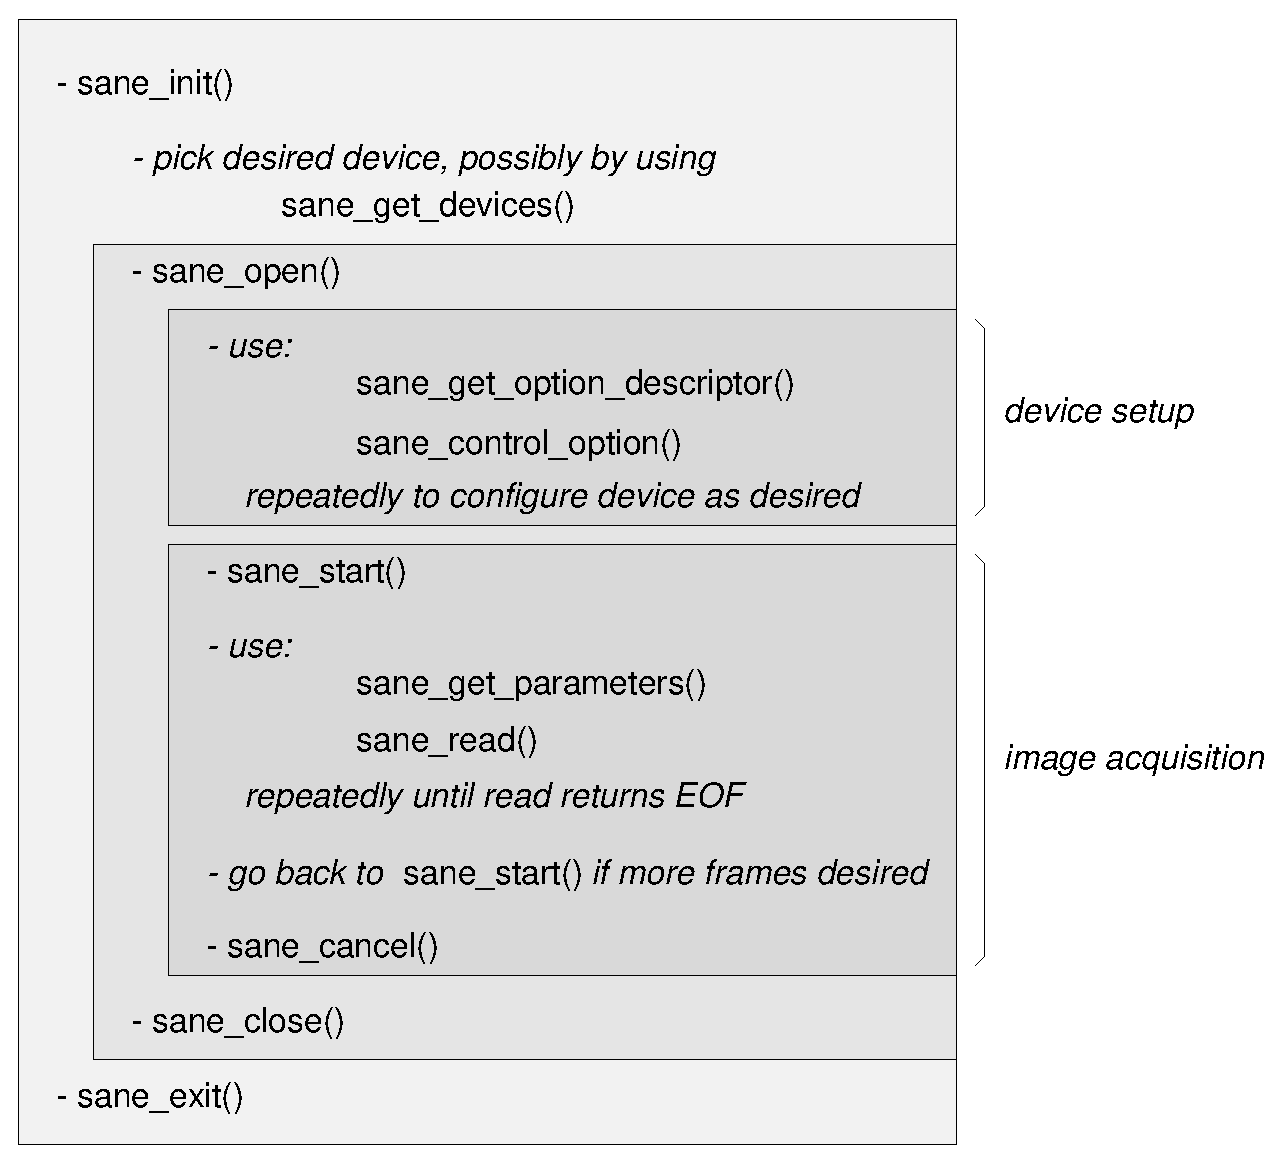
\psfig{file=figs/flow.eps,height=0.5\textheight}
    \caption{Code flow}
    \label{fig:flow}
  \end{center}
\end{figure}

Function \code{sane\_get\_devices()} can be called any time after
\code{sane\_init()} has been called.  It returns the list of the
devices that are known at the time of the call.  This list may change
over time since some devices may be turned on or off or a remote host
may boot or shutdown between different calls.  It should be noted that
this operation may be relatively slow since it requires contacting all
configured devices (some of which may be on remote hosts).  A frontend
may therefore want to provide the ability for a user to directly
select a desired device without requiring a call to this function.

Once a device has been chosen, it is opened using a call to
\code{sane\_open()}.  Multiple devices can be open at any given time.
A SANE backend must not impose artificial constraints on how many
devices can be open at any given time.

An opened device can be setup through the corresponding device handle
using functions \code{sane\_get\_opt\-ion\_desc\-riptor()} and
\code{sane\_control\_option()}.  While setting up a device, obtaining
option descriptors and setting and reading of option values can be
mixed freely.  It is typical for a frontend to read out all available
options at the beginning and then build a dialog (either graphical or
a command-line oriented option list) that allows to control the
available options.  It should be noted that the number of options is
fixed for a given handle.  However, as options are set, other options
may become active or inactive.  Thus, after setting an option, it
maybe necessary to re-read some or all option descriptors.  While
setting up the device, it is also admissible to call
\code{sane\_get\_parameters()} to get an estimate of what the image
parameters will look like once image acquisition begins.

The device handle can be put in blocking or non-blocking mode by a
call to \code{sane\_set\_io\_mode()}.  Devices are required to support
blocking mode (which is the default mode), but support for
non-blocking I/O is strongly encouraged for operating systems such as
UNIX.

After the device is setup properly, image acquisition can be started
by a call to \code{sane\_start()}.  The backend calculates the exact
image parameters at this point.  So future calls to
\code{sane\_get\_parameters()} will return the exact values, rather
than estimates.  Whether the physical image acquisition starts at this
point or during the first call to \code{sane\_read()} is unspecified
by the SANE API.  If non-blocking I/O and/or a select-style interface
is desired, the frontend may attempt to call
\code{sane\_set\_io\_mode()} and/or \code{sane\_get\_select\_fd()} at
this point.  Either of these functions may fail if the backend does
not support the requested operation.

Image data is collected by repeatedly calling \code{sane\_read()}.
Eventually, this function will return an end-of-file status
(\code{SANE\_STATUS\_EOF}).  This indicates the end of the current
frame.  If the frontend expects additional frames (e.g., the
individual channels in of a red/green/blue image or multiple images),
it can call \code{sane\_start()} again.  Once all desired frames have
been acquired, function \code{sane\_cancel()} must be called.  This
operation can also be called at any other time to cancel a pending
operation.  Note that \code{sane\_cancel()} must be called even if the
last read operation returned \code{SANE\_STATUS\_EOF}.

When done using the device, the handle should be closed by a call to
\code{sane\_close()}.  Finally, before exiting the application,
function \code{sane\_exit()} must be called.  It is important not to
forget to call this function since otherwise some resources (e.g.,
temporary files or locks) may remain unclaimed.


\section{Well-Known Options}\index{well-known options}

While most backend options are completely self-describing, there are a
cases where a user interface might want to special-case the handling
of certain options.  For example, the scan area is typically defined
by four options that specify the top-left and bottom-right corners of
the area.  With a graphical user interface, it would be tedious to
force the user to type in these four numbers.  Instead, most such
interfaces will want to present to the user a preview (low-resolution
scan) of the scanner surface and let the user pick the scan area by
dragging a rectangle into the desired position.  For this reason, the
SANE API specifies a small number of option names that have
well-defined meanings.

\subsection{Option Number Count}\index{option count}

Option number 0 has an empty string as its name.  The value of this
option is of type \code{SANE\_TYPE\_INT} and it specifies the total
number of options available for a given device (the count includes
option number 0).  This means that there are two ways of counting the
number of options available: a frontend can either cycle through all
option numbers starting at one until
\code{sane\_get\_option\_descriptor()} returns \code{NULL}, or a
frontend can directly read out the value of option number 0.

\subsection{Scan Resolution Option}\index{scan resolution}\index{resolution option}

Option \code{resolution} is used to select the resolution at which an
image should be acquired.  The type of this option is either
\code{SANE\_TYPE\_INT} or \code{SANE\_TYPE\_FIXED}.  The unit is
\code{SANE\_UNIT\_DPI} (dots/inch).

This option is not mandatory, but if a backend does support it, it
must implement it in a manner consistent with the above definition.

\subsection{Preview Mode Option}\index{preview mode}

The boolean option \code{preview} is used by a frontend to inform the
backend when image acquisition should be optimized for speed, rather
than quality (``preview mode'').  When set to \code{SANE\_TRUE},
preview mode is in effect, when set to \code{SANE\_FALSE} image
acquisition should proceed in normal quality mode.  The setting of
this option \emph{must not\/} affect any other option.  That is, as
far as the other options are concerned, the preview mode is completely
side effect free.  A backend can assume that the frontend will take
care of appropriately setting the scan resolution for preview mode
(through option \code{resolution}).  A backend is free to override the
\code{resolution} value with its own choice for preview mode, but it
is advised to leave this choice to the frontend wherever possible.

This option is not mandatory, but if a backend does support it, it
must implement it in a manner consistent with the above definition.

\subsection{Scan Area Options}\index{scan area options}

The four most important well-known options are the ones that define
the scan area.  The scan area is defined by two points (x/y coordinate
pairs) that specify the top-left and the bottom-right corners.  This
is illustrated in Figure~\ref{fig:area}.  Note that the origin of the
coordinate system is at the top-left corner of the scan surface as
seen by the sensor (which typically is a mirror image of the scan
surface seen by the user).  For this reason, the top-left corner is
the corner for which the abscissa and ordinate values are
simultaneously the {\em smallest} and the bottom-right corner is the
corner for which the abscissa and ordinate values are simulatenously
the {\em largest}.  If this coordinate system is not natural for a
given device, it is the job of the backend to perform the necessary
conversions.
\begin{figure}[tbp]
  \begin{center}
    \leavevmode
    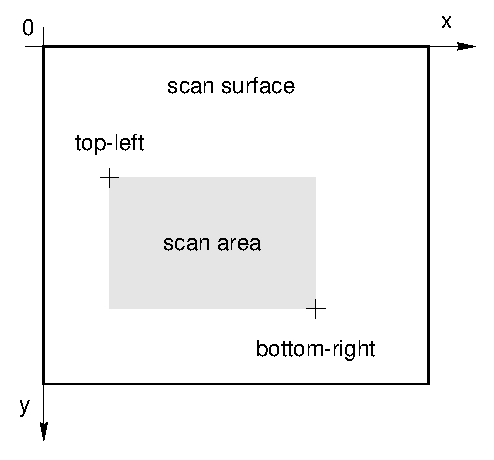
\psfig{file=figs/area.eps,height=0.3\textheight}
    \caption{Scan area options}
    \label{fig:area}
  \end{center}
\end{figure}

The names of the four options that define the scan area are given in
the table below:
\begin{center}
\begin{tabular}{ll}
{\bf Name} & {\bf Description} \\
\code{\defn{tl-x}} & Top-left $x$ coordinate value \\
\code{\defn{tl-y}} & Top-left $y$ coordinate value \\
\code{\defn{br-x}} & Bottom-right $x$ coordinate value \\
\code{\defn{br-y}} & Bottom-right $y$ coordinate value \\
\end{tabular}
\end{center}
There are several rules that should be followed by front and backends
regarding these options:
\begin{itemize}

\item Backends must attach a unit of either pixels
  (\code{SANE\_UNIT\_PIXEL}) or millimeters (\code{SANE\_UNIT\_MM}) to
  these options.  The unit of all four options must be identical.

\item Whenever meaningful, a backend should attach a range or a
  word-list constraint to these options.

\item A frontend can determine the size of the scan surface by first
  checking that the options have range constraints associated.  If a
  range or word-list constraints exist, the frontend can take the
  minimum and maximum values of one of the x and y option
  range-constraints to determine the scan surface size.

\item A frontend must work properly with any or all of these options
  missing.
  
\end{itemize}

\chapter{Network Protocol}\label{chap:net}

The SANE interface has been designed to facilitate network access to
image acquisition devices.  In particular, most SANE implementations
are expected to support a network backend (net client) and a
corresponding network daemon (net server) that allows accessing image
acquisition devices through a network connection.  Network access is
useful in several situations:
\begin{itemize}

\item To provide controlled access to resources that are inaccessible
  to a regular user.  For example, a user may want to access a device
  on a host where she has no account on.  With the network protocol,
  it is possible to allow certain users to access scanners without
  giving them full access to the system.

  Controlling access through the network daemon can be useful even in
  the local case: for example, certain backends may require root
  privileges to access a device.  Rather than installing each frontend
  as setuid-root, a system administrator could instead install the
  SANE network daemon as setuid-root.  This enables regular users to
  access the privileged device through the SANE daemon (which,
  presumably, supports a more fine-grained access control mechanism
  than the simple setuid approach).  This has the added benefit that
  the system administrator only needs to trust the SANE daemon, not
  each and every frontend that may need access to the privileged
  device.

\item Network access provides a sense of ubiquity of the available
  image acquisition devices.  For example, in a local area network
  environment, this allows a user to log onto any machine and have
  convenient access to any resource available to any machine on the
  network (subject to permission constraints).

\item For devices that do not require physical access when used (e.g.,
  video cameras), network access allows a user to control and use
  these devices without being in physical proximity.  Indeed, if such
  devices are connected to the Internet, access from any place in the
  world is possible.

\end{itemize}

The network protocol described in this chapter has been design with
the following goals in mind:
\begin{enumerate}

\item Image transmission should be efficient (have low encoding
  overhead).

\item Accessing option descriptors on the client side must be
  efficient (since this is a very common operation).

\item Other operations, such as setting or inquiring the value of an
  option are less performance critical since they typically require
  explicit user action.

\item The network protocol should be simple and easy to implement on
  any host architecture and any programming language.

\end{enumerate}
The SANE protocol can be run across any transport protocol that
provides reliable data delivery.  While SANE does not specify a
specific transport protocol, it is expected that TCP/IP will be among
the most commonly used protocols.

\section{Data Type Encoding}

\subsection{Primitive Data Types}

The four primitive types of the SANE standard are encoded as follows:
\begin{description}

\item[\code{\defn{SANE\_Byte}}:] A byte is encoded as an 8 bit value.
  Since the transport protocol is assumed to be byte-orientd, the bit
  order is irrelevant.

\item[\code{\defn{SANE\_Word}}:] A word is encoded as 4 bytes (32
  bits).  The bytes are ordered from most-significant to
  least-significant byte (big-endian byte-order).

\item[\code{\defn{SANE\_Char}}:] A character is currently encoded as an 8-bit
  ISO LATIN-1 value.  An extension to support wider character sets (16 or 32
  bits) is planned for the future, but not supported at this point.

\item[\code{\defn{SANE\_String}}:] A string pointer is encoded as a
  \code{SANE\_Char} array.  The trailing NUL byte is considered part
  of the array and a \code{NULL} pointer is encoded as a zero-length
  array.
  
\item[\code{\defn{SANE\_Handle}}:] A handle is encoded like a word.
  The network backend needs to take care of converting these integer
  values to the opaque pointer values that are presented to the user
  of the network backend.  Similarly, the SANE daemon needs to take
  care of converting the opaque pointer values it receives from its
  backends into 32-bit integers suitable for use for network encoding.

\item[{\em\defn{enumeration types}}:] Enumeration types are encoded
  like words.

\end{description}

\subsection{Type Constructors}

Closely following the type constructors of the C language, the SANE network
protocol supports the following four constructors:
\begin{description}

\item[{\em\defn{pointer}}:] A pointer is encoded by a word that indicates
  whether the pointer is a NULL-pointer which is then followed by the
  value that the pointer points to (in the case of a non-NULL pointer;
  in the case of a NULL pointer, no bytes are encoded for the pointer
  value).

\item[{\em\defn{array}}:] An array is encoded by a word that indicates
  the length of the array followed by the values of the elements in
  the array.  The length may be zero in which case no bytes are
  encoded for the element values.

\item[{\em\defn{structure}}:] A structure is encoded by simply encoding the
  structure members in the order in which they appear in the
  corresponding C type declaration.

\item[{\em\defn{union}}:] A union must always be accompanied by a tag
  value that indicates which of the union members is the currently the
  active one.  For this reason, the union itself is encoded simply by
  encoding the value of the currently active member.

\end{description}

Note that for type constructors, the pointer, element, or member
values themselves may have a constructed type.  Thus, the above rules
should be applied recursively until a sequence of primitive types has
been found.

Also SANE had no need for encoding of circular structures.  This
greatly simplifies the network protocol.

\section{Remote Procedure Call Requests}

The SANE network protocol is a client/server-style remote procedure
call (RPC) protocol.  This means that all activity is initiated by the
client side (the network backend)---a server is restricted to
answering request by the client.

\subsection{\code{\defn{SANE\_NET\_INIT}}}

This RPC establishes a connection to a particular SANE network daemon.
It must be the first call in a SANE network session.  The parameter
and reply arguments for this call are shown in the table below:
\begin{center}
\begin{tabular}{ll}
  {\bf request:} & {\bf reply:} \\
  \code{SANE\_Word version\_code} & \code{SANE\_Word status} \\
  \code{SANE\_String user\_name}   & \code{SANE\_Word version\_code} \\
\end{tabular}
\end{center}
The \code{version\_code} argument in the request is the SANE
version-code of the network backend that is contacting the network
daemon (see Section~\ref{sec:saneversioncode}).  The
``build-revision'' in the version code is used to hold the network
protocol version.  The SANE network daemon receiving such a request
must make sure that the network protocol version corresponds to a
supported version since otherwise the encoding of the network stream
may be incompatible (even though the SANE interface itself may be
compatible).  The \code{user\_name} argument is the name of the user
on whose behalf this call is being performed.  If the network backend
cannot determine a user-name, it passes a \code{NULL} pointer for this
argument.  No trust should be placed in the authenticity of this
user-name.  The intent of this string is to provide more convenience
to the user.  E.g., it could be used as the default-user name in
subsequent authentication calls.

In the reply, \code{status} indicates the completion status.  If the
value is anything other than \code{SANE\_STA\-TUS\_SUCCESS}, the
remainder of the reply has undefined values.\footnote{The sane network
  daemon should be careful not to leak information in the undefined
  portion of the reply.} The \code{version\_code} argument returns the
SANE version-code that the network daemon supports.  See the comments
in the previous paragraph on the meaning of the build-revision in this
version code.

\subsection{\code{\defn{SANE\_NET\_GET\_DEVICES}}}

This RPC is used to obtain the list of devices accessible by the SANE
daemon.
\begin{center}
\begin{tabular}{ll}
  {\bf request:} & {\bf reply:} \\
  \code{void} & \code{SANE\_Word status} \\
              & \code{SANE\_Device ***device\_list} \\
\end{tabular}
\end{center}
There are no arguments in the request for this call.

In the reply, \code{status} indicates the completion status.  If the
value is anything other than \code{SANE\_STA\-TUS\_SUCCESS}, the
remainder of the reply has undefined values.  The \code{device\_list}
argument is a pointer to a \code{NULL}-terminated array of
\code{SANE\_Device} pointers.

\subsection{\code{\defn{SANE\_NET\_OPEN}}}

This RPC is used to open a connection to a remote SANE device.
\begin{center}
\begin{tabular}{ll}
  {\bf request:} & {\bf reply:} \\
  \code{SANE\_String device\_name} & \code{SANE\_Word status} \\
                                   & \code{SANE\_Word handle} \\
                                   & \code{SANE\_String resource} \\
\end{tabular}
\end{center}
The \code{device\_name} argument specifies the name of the device to
open.

In the reply, \code{status} indicates the completion status.  If the
value is anything other than \code{SANE\_STA\-TUS\_SUCCESS}, the
remainder of the reply has undefined values.  The \code{handle}
argument specifies the device handle that uniquely identifies the
connection.  The \code{resource} argument is used to request
authentication.  If it has a non-\code{NULL} value, the network
backend should authenticate the specified resource and then retry this
operation (see Section~\ref{sec:authorization} for details on how to
authorize a resource).

\subsection{\code{\defn{SANE\_NET\_CLOSE}}}

This RPC is used to close a connection to a remote SANE device.
\begin{center}
\begin{tabular}{ll}
  {\bf request:} & {\bf reply:} \\
  \code{SANE\_Word handle} & \code{SANE\_Word dummy} \\
\end{tabular}
\end{center}
The \code{handle} argument identifies the connection that should be
closed.

In the reply, the \code{dummy} argument is unused.  Its purpose is to
ensure proper synchronization (without it, a net client would not be
able to determine when the RPC has completed).

\subsection{\code{\defn{SANE\_NET\_GET\_OPTION\_DESCRIPTORS}}}

This RPC is used to obtain {\em all\/} the option descriptors for a
remote SANE device.
\begin{center}
\begin{tabular}{ll}
  {\bf request:} & {\bf reply:} \\
  \code{SANE\_Word handle} & \code{Option\_Descriptor\_Array odesc} \\
\end{tabular}
\end{center}
The \code{handle} argument identifies the remote device whose option
descriptors should be obtained.

In the reply, the \code{odesc} argument is used to return the array of
option descriptors.  The option descriptor array has the following
structure:
\begin{quote}\index{Option\_Descriptor\_Array}
\begin{verbatim}
struct Option_Descriptor_Array
  {
    SANE_Word num_options;
    SANE_Option_Descriptor **desc;
  };
\end{verbatim}
\end{quote}


\subsection{\code{\defn{SANE\_NET\_CONTROL\_OPTION}}}

This RPC is used to control (inquire, set, or set to automatic) a
specific option of a remote SANE device.
\begin{center}
\begin{tabular}{ll}
  {\bf request:} & {\bf reply:} \\
  \code{SANE\_Word handle}      & \code{SANE\_Status status} \\
  \code{SANE\_Word option}      & \code{SANE\_Word info} \\
  \code{SANE\_Word action}      & \code{SANE\_Word value\_type} \\
  \code{SANE\_Word value\_type} & \code{SANE\_Word value\_size} \\
  \code{SANE\_Word value\_size} & \code{void *value} \\
  \code{void *value}            & \code{SANE\_String *resource} \\
\end{tabular}
\end{center}
The \code{handle} argument identifies the remote device whose option
should be controlled.  Argument \code{option} is the number (index) of
the option that should be controlled.  Argument \code{action}
specifies what action should be taken (get, set, or set automatic).
Argument \code{value\_type} specifies the type of the option value
(must be one of \code{SANE\_TYPE\_BOOL}, \code{SANE\_TYPE\_INT},
\code{SANE\_TYPE\_FIXED}, \code{SANE\_TYPE\_STR\-ING},
\code{SANE\_TYPE\_BUTTON}).  Argument \code{value\_size} specifies
the size of the option value in number of bytes (see
Section~\ref{sec:valuesize} for the precise meaning of this value).
Finally, argument \code{value} is a pointer to the option value.  It
must be a writeable area that is at least \code{value\_size} bytes
large. (Note that this area must be writable even if the action is to
set the option value.  This is because the backend may not be able to
set the exact option value, in which case the option value is used to
return the next best value that the backend has chosen.)

In the reply, argument \code{resource} is set to the name of the
resource that must be authorized before this call can be retried.  If
this value is non-\code{NULL}, all other arguments have undefined
values (see Section~\ref{sec:authorization} for details on how to
authorize a resource).  Argument \code{status} indicates the
completion status.  If the value is anything other than
\code{SANE\_STA\-TUS\_SUCCESS}, the remainder of the reply has undefined
values.  The \code{info} argument returns the information on how well
the backend was able to satisfy the request.  For details, see the
description of the corresponding argument in
Section~\ref{sec:control}.  Arguments \code{value\_type} and
\code{value\_size} have the same values as the arguments by the same
name in corresponding request.  The values are repeated here to ensure
that both the request and the reply are self-contained (i.e., they can
be encoded and decoded independently).  Argument \code{value} is holds
the value of the option that has become effective as a result of this
RPC.


\subsection{\code{\defn{SANE\_NET\_GET\_PARAMETERS}}}

This RPC is used to obtain the scan parameters of a remote SANE
device.
\begin{center}
\begin{tabular}{ll}
  {\bf request:} & {\bf reply:} \\
  \code{SANE\_Word handle} & \code{SANE\_Status status} \\
                           & \code{SANE\_Parameters params} \\
\end{tabular}
\end{center}
The \code{handle} argument identifies the connection to the remote
device whose scan parameters should be returned.

In the reply, \code{status} indicates the completion status.  If the
value is anything other than \code{SANE\_STA\-TUS\_SUC\-CESS}, the
remainder of the reply has undefined values.  The argument
\code{params} is used to return the scan parameters.

\subsection{\code{\defn{SANE\_NET\_START}}}

This RPC is used to start image acquisition (scanning).
\begin{center}
\begin{tabular}{ll}
  {\bf request:} & {\bf reply:} \\
  \code{SANE\_Word handle} & \code{SANE\_Status status} \\
                           & \code{SANE\_Word port} \\
                           & \code{SANE\_Word byte\_order} \\
                           & \code{SANE\_String resource} \\
\end{tabular}
\end{center}
The \code{handle} argument identifies the connection to the remote
device from which the image should be acquired.

In the reply, argument \code{resource} is set to the name of the
resource that must be authorized before this call can be retried.  If
this value is non-\code{NULL}, all other arguments have undefined
values (see Section~\ref{sec:authorization} for details on how to
authorize a resource).  Argument, \code{status} indicates the
completion status.  If the value is anything other than
\code{SANE\_STA\-TUS\_SUCCESS}, the remainder of the reply has
undefined values.  The argument \code{port} returns the port number
from which the image data will be available.  To read the image data,
a network client must connect to the remote host at the indicated port
number.  Through this port, the image data is transmitted as a
sequence of data records.  Each record starts with the data length in
bytes.  The data length is transmitted as a sequence of four bytes.
These bytes should be interpreted as an unsigned integer in big-endian
format.  The four length bytes are followed by the number of data
bytes indicated by the length.  Except for byte-order, the data is in
the same format as defined for \code{sane\_read()}.  Since some
records may contain no data at all, a length value of zero is
perfectly valid.  The special length value of \code{0xffffffff} is
used to indicate the end of the data stream.  That is, after receiving
a record length of \code{0xffffffff}, the network client should close
the data connection and stop reading data.

Argument \code{byte\_order} specifies the byte-order of the image
data.  A value of 0x1234 indicates little-endian format, a value of
0x4321 indicates big-endian format.  All other values are presently
undefined and reserved for future enhancements of this protocol.  The
intent is that a network server sends data in its own byte-order and
the client is responsible for adjusting the byte-order, if necessary.
This approach causes no unnecessary overheads in the case where the
server and client byte-order match and puts the extra burden on the
client side when there is a byte-order mismatch.  Putting the burden
on the client-side improves the scalability properties of this
protocol.

\subsection{\code{\defn{SANE\_NET\_CANCEL}}}

This RPC is used to cancel the current operation of a remote SANE
device.
\begin{center}
\begin{tabular}{ll}
  {\bf request:} & {\bf reply:} \\
  \code{SANE\_Word handle} & \code{SANE\_Word dummy} \\
\end{tabular}
\end{center}
The \code{handle} argument identifies the connection whose operation
should be cancelled.

In the reply, the \code{dummy} argument is unused.  Its purpose is to
ensure proper synchronization (without it, a net client would not be
able to determine when the RPC has completed).

\subsection{\code{\defn{SANE\_NET\_AUTHORIZE}}}\label{sec:authorization}
\index{network authorization}

This RPC is used to pass authorization data from the net client to the
net server.
\begin{center}
\begin{tabular}{ll}
  {\bf request:} & {\bf reply:} \\
  \code{SANE\_String resource} & \code{SANE\_Word dummy} \\
  \code{SANE\_String username} & \\
  \code{SANE\_String password} & \\
\end{tabular}
\end{center}
The \code{resource} argument specifies the name of the resource to be
authorized.  This argument should be set to the string returned in the
\code{resource} argument of the RPC reply that required this
authorization call.  The \code{username} and \code{password} are the
name of the user that is accessing the resource and the password for
the specified resource/user pair.

Since the password is not encrypted during network transmission, it is
recommended to use the following extension:

If the server adds the string `\code{\$MD5\$}' to the resource-name followed
by a random string not longer then 128 bytes, the client may answer with the
MD5 digest of the concatenation of the password and the random string. To
differentiate between the MD5 digest and a strange password the client prepends
the MD5 digest with the string `\code{\$MD5\$}'.

In the reply, \code{dummy} is completely unused.  Note that there is
no direct failure indication.  This is unnecessary since a net client
will retry the RPC that resulted in the authorization request until
that call succeeds (or until the request is cancelled). The RPC that resulted
in the authorization request continues after the reply from the client and may
fail with \code{SANE\_STATUS\_ACCESS\_DENIED}.


\subsection{\code{\defn{SANE\_NET\_EXIT}}}

This RPC is used to disconnect a net client from a net server.  There
are no request or reply arguments in this call.  As a result of this
call, the connection between the client and the server that was
established by the \code{SANE\_NET\_INIT} call will be closed.

% Local Variables: 
% mode: latex
% TeX-master: "sane.tex"
% End: 


\chapter{Contact Information}\label{chap:contact}

The SANE standard is discussed and evolved via a mailing list.
Anybody with email access to the Internet can automatically join and
leave the discussion group by sending mail to the following address.
\begin{quote}\index{mailing list}
\begin{verbatim}
majordomo@mostang.com
\end{verbatim}
\end{quote}
To subscribe, send a mail with the body ``\verb|subscribe sane-devel|'' to the
above address.

A complete list of commands supported can be obtained by sending a
mail with a subject of ``\code{help}'' to the above address.  The
mailing list is archived and available through the SANE home page at
URL:
\begin{quote}
\url{http://www.mostang.com/sane/}
\end{quote}

\newpage
\documentclass[11pt,DVIps]{report}

\usepackage{times,epsfig,changebar,html}

\setlength{\parindent}{0pt}
\setlength{\parskip}{1.5ex plus 0.5ex minus 0.5ex}
\setlength{\textwidth}{6.5in}
\setlength{\textheight}{8.5in}
\setlength{\marginparwidth}{0pt}
\setlength{\oddsidemargin}{0pt}
\setlength{\evensidemargin}{0pt}
\setlength{\marginparsep}{0pt}
\addtolength{\topmargin}{-0.75in}

\title{\huge SANE Standard Version 1.02}
\author{}
\date{February 19, 2002} 

\makeindex

\begin{document}

\newcommand{\filename}[1]{{\tt #1}}
\newcommand{\code}[1]{{\tt #1}}
\newcommand{\var}[1]{{\it #1}}
\newcommand{\defn}[1]{#1\index{#1}}

\begin{latexonly}
  \setcounter{changebargrey}{0}   % black change bars
\end{latexonly}

\maketitle
\tableofcontents
\listoffigures
\listoftables


\chapter{Preface}

The SANE standard is being developed by a group of free-software
developers.  The process is open to the public and comments as well as
suggestions for improvements are welcome.  Information on how to join
the SANE development process can be found in Chapter
\ref{chap:contact}.

The SANE standard is intended to streamline software development by
providing a standard application programming interface to access
raster scanner hardware.  This should reduce the number of different
driver implementations, thereby reducing the need for reimplementing
similar code.


\section{About This Document}

This document is intended for developers who are creating either an
application that requires access to raster scanner hardware and for
developers who are implementing a SANE driver.  It does not cover
specific implementations of SANE components.  Its sole purpose is to
describe and define the SANE application interface that will enable
any application on any platform to interoperate with any SANE backend
for that platform.

The remainder of this document is organized as follows.
Chapter~\ref{chap:intro} provides introductional material.
Chapter~\ref{chap:environ} presents the environment SANE is designed
for.  Chapter~\ref{chap:api} details the SANE Application Programmer
Interface.  Chapter~\ref{chap:net} specifies the network protocol that
can be used to implement the SANE API in a network transparent
fashion.  Finally, Chapter~\ref{chap:contact} gives information on how
to join the SANE development process.

\subsection{Typographic Conventions}

Changes since the last revision of this document are highlighted
like this:

% \begin{changebar}
%   Paragraphs that changed since the last revision of the documention
%   are marked like this paragraph.
% \end{changebar}

\chapter{Introduction}\label{chap:intro}

SANE is an application programming interface (API) that provides
standardized access to any raster image scanner hardware.  The
standardized interface allows to write just one driver for each
scanner device instead of one driver for each scanner and application.
The reduction in the number of required drivers provides significant
savings in development time.  More importantly, SANE raises the level
at which applications can work.  As such, it will enable applications
that were previously unheard of in the UNIX world.  While SANE is
primarily targeted at a UNIX environment, the standard has been
carefully designed to make it possible to implement the API on
virtually any hardware or operating system.

SANE is an acronym for ``Scanner Access Now Easy.''  Also, the hope is
that SANE is sane in the sense that it will allow easy implementation
of the API while accommodating all features required by today's
scanner hardware and applications.  Specifically, SANE should be broad
enough to accommodate devices such as scanners, digital still and
video cameras, as well as virtual devices like image file filters.

\section{Terminology}

An application that uses the SANE interface is called a SANE {\em
  frontend}.  A driver that implements the SANE interface is called a
SANE {\em backend}.  A {\em meta backend\/} provides some means to
manage one or more other backends.


\chapter{The SANE Environment}\label{chap:environ}

SANE is defined as a C-callable library interface.  Accessing a raster
scanner device typically consists of two phases: first, various
controls of the scanner need to be setup or queried.  In the second
phase, one or more images are acquired.

Since the device controls are widely different from device to device,
SANE provides a generic interface that makes it easy for a frontend to
give a user access to all controls without having to understand each
and every device control.  The design principle used here is to
abstract each device control into a SANE {\em option\/}.  An option is
a self-describing name/value pair.  For example, the brightness
control of a camera might be represented by an option called
\code{brightness} whose value is an integer in the range from 0 to
255.

With self-describing options, a backend need not be concerned with
{\em presentation\/} issues: the backend simply provides a list of
options that describe all the controls available in the device.
Similarly, there are benefits to the frontend: it need not be
concerned with the {\em meaning\/} of each option.  It simply provides
means to present and alter the options defined by the backend.


\section{Attaching to a SANE backend}

The process through which a SANE frontend connects to a backend is
platform dependent.  Several possibilities exist:
\begin{itemize}

\item {\bf Static linking:} A SANE backend may be linked directly into
  a frontend.  While the simplest method of attaching to a backend, it
  is somewhat limited in functionality since the available devices is
  limited to the ones for which support has been linked in when the
  frontend was built.  But even so static linking can be quite useful,
  particularly when combined with a backend that can access scanners
  via a network.  Also, it is possible to support multiple backends
  simultaneously by implementing a meta backend that manages several
  backends that have been compiled in such a manner that they export
  unique function names.  For example, a backend called \code{be}
  would normally export a function called \code{sane\_read()}.  If
  each backend would provide such a function, static linking would
  fail due to multiple conflicting definitions of the same symbol.
  This can be resolved by having backend \code{be} include a
  header file that has lines of the form:
  \begin{quote}
\begin{verbatim}
#define sane_read be_sane_read
\end{verbatim}
  \end{quote}
  With definitions of this kind, backend \code{be} will export
  function name \code{be\_sane\_read()}.  Thus, all backends will
  export unique names.  As long as a meta backend knows about these
  names, it is possible to combine several backends at link time and
  select and use them dynamically at runtime.

\item {\bf Dynamic linking:} A simpler yet more powerful way to
  support multiple backends is to exploit dynamic linking on platforms
  that support it.  In this case, a frontend is linked against a
  shared library that implements any SANE backend.  Since each
  dynamically linked backend exports the same set of global symbols
  (all starting with the prefix \code{sane\_}), the dynamic library
  that gets loaded at runtime does not necessarily have to be the same
  one as one the frontend got linked against.  In other words, it is
  possible to switch the backend by installing the appropriate backend
  dynamic library.

  More importantly, dynamic linking makes it easy to implement a meta
  backend that loads other backends {\em on demand}.  This is a
  powerful mechanism since it allows adding new backends merely by
  installing a shared library and updating a configuration file.

\item {\bf Network connection:} Arguably the ultimate way to attach to
  a scanner is by using the network to connect to a backend on a
  remote machine.  This makes it possible to scan images from any host
  in the universe, as long as there is a network connection to that
  host and provided the user is permitted to access that scanner.

\end{itemize}

\begin{figure}[htbp]
  \begin{center}
    \leavevmode
    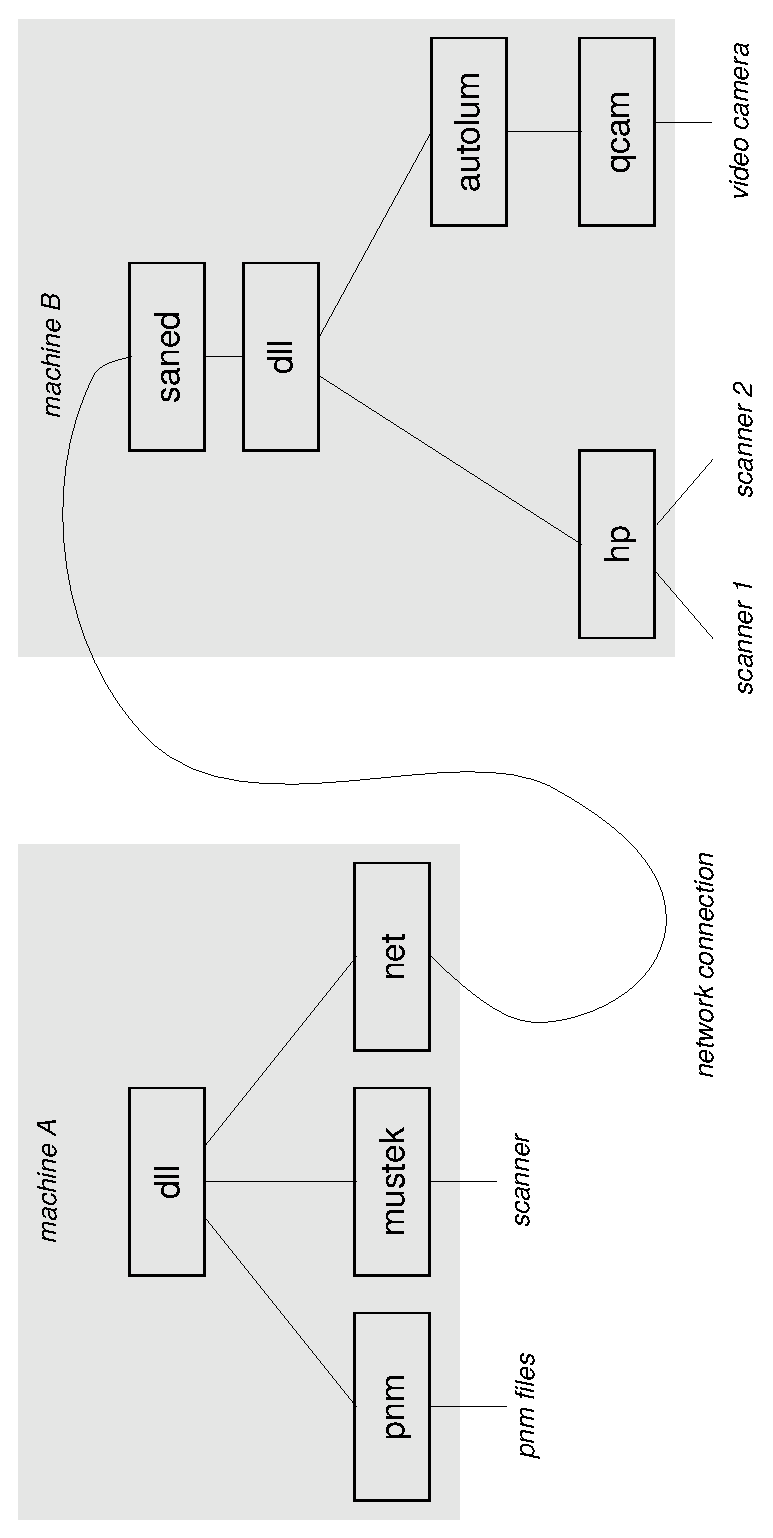
\psfig{file=figs/hierarchy.eps,angle=270,width=\textwidth}
    \caption{Example SANE Hiearchy}
    \label{fig:hierarchy}
  \end{center}
\end{figure}

The above discussion lists just a few ways for frontends to attach to
a backend.  It is of course possible to combine these solutions to
provide an entire hierarchy of SANE backends.  Such a hierarchy is
depicted in Figure~\ref{fig:hierarchy}.  The figure shows that machine
A uses a dynamic-linking based meta backend called \code{dll} to
access the backends called \code{pnm}, \code{mustek}, and \code{net}.
The first two are real backends, whereas the last one is a meta
backend that provides network transparent access to remote scanners.
In the figure, machine B provides non-local access to its scanners
through the SANE frontend called \code{saned}.  The \code{saned} in
turn has access to the \code{hp} and \code{autolum} backends through
another instance of the \code{dll} backend.  The \code{autolum} meta
backend is used to automatically adjust the luminance (brightness) of
the image data acquired by the camera backend called \code{qcam}.

Note that a meta backend really is both a frontend and a backend at
the same time.  It is a frontend from the viewpoint of the backends
that it manages and a backend from the viewpoint of the frontends that
access it.  The name ``meta backend'' was chosen primarily because the
SANE standard describes the interface from the viewpoint of a (real)
frontend.


\section{Image Data Format}\label{sec:imageformat}\index{image data format}

Arguably the most important aspect of an image acquisition system is
how images are represented.  The SANE approach is to define a simple
yet powerful representation that is sufficient for vast majority of
applications and devices.  While the representation is simple, the
interface has been defined carefully to allow extending it in the
future without breaking backwards compatibility.  Thus, it will be
possible to accommodate future applications or devices that were not
anticipated at the time this standard was created.

A SANE image is a rectangular area.  The rectangular area is
subdivided into a number of rows and columns.  At the intersection of
each row and column is a quadratic pixel.  A pixel consists of one or
more sample values.  Each sample value represents one channel (e.g.,
the red channel).  Each sample value has a certain bit depth.  The bit
depth is fixed for the entire image and can be as small as one bit.
Valid bit depths are 1, 8, or 16 bits per sample.  If a device's
natural bit depth is something else, it is up to the driver to scale
the sample values appropriately (e.g., a 4 bit sample could be scaled
by a factor of four to represent a sample value of depth 8).

\subsection{Image Transmission}

The SANE API transmits an image as a sequence of frames.  Each frame
covers the same rectangular area as the entire image, but may contain
only a subset of the channels in the final image.  For example, a
red/green/blue image could either be transmitted as a single frame
that contains the sample values for all three channels or it could be
transmitted as a sequence of three frames: the first frame containing
the red channel, the second the green channel, and the third the blue
channel.

Conceptually, each frame is transmitted a byte at a time.  Each byte
may contain 8 sample values (for an image bit depth of 1), one full
sample value (for an image bit depth of 8), or a partial sample value
(for an image bit depth of 16 or bigger).  In the latter case, the
bytes of each sample value are transmitted in the machine's native
byte order.
\begin{quote}
  \begin{center}
    {\bf Backend Implementation Note}
  \end{center}
  A network-based meta backend will have to ensure that the byte order
  in image data is adjusted appropriately if necessary.  For example,
  when the meta backend attaches to the server proxy, the proxy may
  inform the backend of the server's byte order.  The backend can then
  apply the adjustment if necessary.  In essence, this implements a
  ``receiver-makes-right'' approach.
\end{quote}

\begin{figure}[htbp]
  \begin{center}
    \leavevmode
    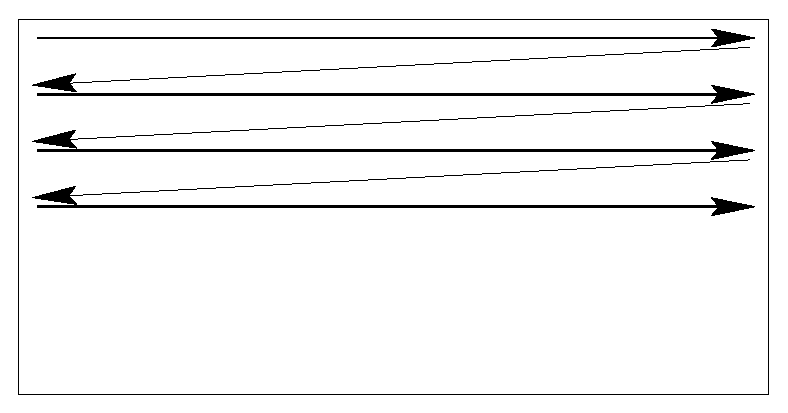
\psfig{file=figs/xfer.eps,width=0.5\textwidth}
    \caption{Transfer order of image data bytes}
    \label{fig:xfer}
  \end{center}
\end{figure}

The order in which the sample values in a frame are transmitted is
illustrated in Figure~\ref{fig:xfer}.  As can be seen, the values are
transmitted row by row and each row is transmitted from left-most to
right-most column.  The left-to-right, top-to-bottom transmission
order applies when the image is viewed in its normal orientation (as
it would be displayed on a screen, for example).

If a frame contains multiple channels, then the channels are
transmitted in an interleaved fashion.  Figure~\ref{fig:pixels}
illustrates this for the case where a frame contains a complete
red/green/blue image with a bit-depth of 8.  For a bit depth of 1,
each byte contains 8 sample values of a {\em single\/} channel.  In
other words, a bit depth 1 frame is transmitted in a byte interleaved
fashion.

\begin{figure}[htbp]
  \begin{center}
    \leavevmode
    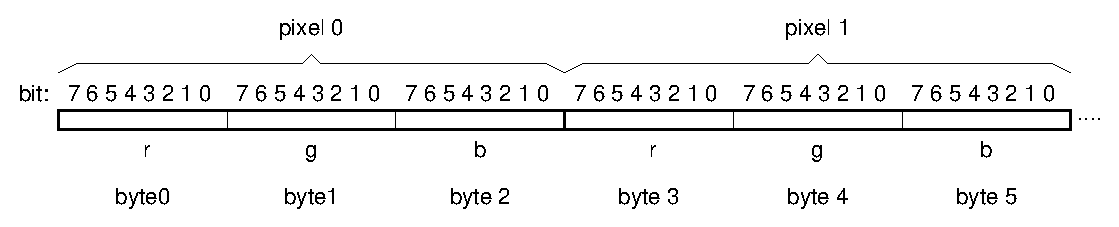
\psfig{file=figs/image-data.eps,width=0.8\textwidth}
    \caption{Bit and byte order or image data}
    \label{fig:pixels}
  \end{center}
\end{figure}

When transmitting an image frame by frame, the frontend needs to know
what part of the image a frame represents (and how many frames it
should expect).  For that purpose, the SANE API tags every frame with
a type.  This version of the SANE standard supports the following
frame types:
\begin{quote}
\begin{description}

\item[\code{\defn{SANE\_FRAME\_GRAY}}:] The frame contains a single
  channel of data that represents sample values from a spectral band
  that covers the human visual range.  The image consists of this
  frame only.

\item[\code{\defn{SANE\_FRAME\_RGB}}:] The frame contains three
  channels of data that represent sample values from the red, green,
  and blue spectral bands.  The sample values are interleaved in the
  order red, green, and blue.  The image consists of this frame only.

\item[\code{\defn{SANE\_FRAME\_RED}}:] The frame contains one channel
  of data that represents sample values from the red spectral band.
  The complete image consists of three frames:
  \code{SANE\_\-FRA\-ME\_RED}, \code{SANE\_FRAME\_GREEN}, and
  \code{SANE\_FRAME\_BLUE}.  The order in which the frames are
  transmitted chosen by the backend.

\item[\code{\defn{SANE\_FRAME\_GREEN}}:] The frame contains one
  channel of data that represents sample values from the green
  spectral band.  The complete image consists of three frames:
  \code{SANE\_\-FRA\-ME\_RED}, \code{SANE\_FRAME\_GREEN}, and
  \code{SANE\_FRAME\_BLUE}.  The order in which the frames are
  transmitted chosen by the backend.

\item[\code{\defn{SANE\_FRAME\_BLUE}}:] The frame contains one channel
  of data that represents sample values from the blue spectral band.
  The complete image consists of three frames:
  \code{SANE\_\-FRA\-ME\_RED}, \code{SANE\_FRAME\_GREEN}, and
  \code{SANE\_FRAME\_BLUE}.  The order in which the frames are
  transmitted chosen by the backend.

\end{description}
\end{quote}

In frames of type SANE\_FRAME\_GRAY, when the bit depth is 1 there are
only two sample values possible, 1 represents minimum intensity
(black) and 0 represents maximum intensity (white).  For all other bit
depth and frame type combinations, a sample value of 0 represents
minimum intensity and larger values represent increasing intensity.


\chapter{The SANE Application Programmer Interface (API)}\label{chap:api}

This Section defines version 1 of the SANE application
programmer interface (API).  Any SANE frontend must depend on the
interface defined in this section only.  Converseley, any SANE backend
must implement its functionality in accordance with this
specification.  The interface as documented here is declared as a C
callable interface in a file called \filename{sane/sane.h}.  This file should
normally be included via a C pre-processor directive of the form:
\begin{verbatim}
  #include <sane/sane.h>
\end{verbatim}


\section{Version Control}

The SANE standard is expected to evolve over time.  Whenever a change
to the SANE standard is made that may render an existing frontend or
backend incompatible with the new standard, the major version number
must be increased.  Thus, any frontend/backend pair is compatible
provided the major version number of the SANE standard they implement
is the same.  A frontend may implement backwards compatiblity by
allowing major numbers that are smaller than the expected major number
(provided the frontend really can cope with the older version).  In
contrast, a backend always provides support for one and only one
version of the standard.  If a specific application does require that
two different versions of the same backend are accessible at the same
time, it is possible to do so by installing the two versions under
different names.

SANE version control also includes a minor version number and a build
revision.  While control of these numbers remains with the implementor
of a backend, the recommended use is as follows.  The minor version is
incremented with each official release of a backend.  The build
revision is increased with each build of a backend.

The SANE API provides the following five macros to manage version
numbers.
\begin{quote}
  \begin{description}
  \item[\code{\defn{SANE\_CURRENT\_MAJOR}}:] The value of this macro is the
    number of the SANE standard that the interface implements.

  \item[\code{\defn{SANE\_VERSION\_CODE}(\var{maj},\var{min},\var{bld})}:]
    \label{sec:saneversioncode}
    This macro can be used to build a monotonically increasing version
    code.  A SANE version code consists of the SANE standard major
    version number (\var{maj}), the minor version number \var{min},
    and the build revision of a backend (\var{bld}).  The major and
    minor version numbers must be in the range 0\ldots255 and the
    build revision must be in the range 0\ldots65535.

    Version codes are monotonic in the sense that it is possible to
    apply relational operators (e.g., equality or less-than test)
    directly on the version code rather than individually on the three
    components of the version code.

    Note that the major version number alone determines whether a
    frontend/backend pair is compatible.  The minor version and the
    build revision are used for informational and bug-fixing purposes
    only.
  
  \item[\code{\defn{SANE\_VERSION\_MAJOR}(\var{vc})}:] This macro returns the
    major version number component of the version code passed in
    argument \var{vc}.
  \item[\code{SANE\_VERSION\_MINOR(\var{vc})}:] This macro returns the
    minor version number component of the version code passed in
    argument \var{vc}.
  \item[\code{SANE\_VERSION\_BUILD(\var{vc})}:] This macro returns the
    build revision component of the version code passed in argument
    \var{vc}.
  \end{description}
\end{quote}


\section{Data Types}

\subsection{Base Types}

The SANE standard is based on just two SANE-specific base types: the
SANE byte and word.
\begin{quote}
  \code{typedef \var{some-scalar-type\/} \defn{SANE\_Byte};} \\
  \code{typedef \var{some-scalar-type\/} \defn{SANE\_Word};}
\end{quote}
\verb|SANE_Byte| must correspond to some scalar C type that is capable
of holding values in the range 0 to 255.  \verb|SANE_Word| must be
capable of holding any of the following:
\begin{itemize}
  \item the truth values \verb|SANE_FALSE| and \verb|SANE_TRUE|
  \item signed integers in the range $-2^{31}\ldots2^{31}-1$
  \item fixed point values in the range $-32768\ldots32767.9999$ with
    a resolution of $1/65536$
  \item 32 bits (for bit sets)
\end{itemize}
Note that the SANE standard does not define what C type
\verb|SANE_Byte| and \verb|SANE_Word| map to.  For example, on some
platforms, the latter may map to \verb|long int| whereas on others it
may map to \verb|int|.  A portable SANE frontend or backend must
therefore not depend on a particular mapping.

\subsection{Boolean Type}

\code{\defn{SANE\_Bool}} is used for variables that can take one of
the two truth values \code{\defn{SANE\_FALSE}} and
\code{\defn{SANE\_TRUE}}.  The former value is defined to be 0,
whereas the latter is 1.\footnote{This is different from ANSI C where
  any non-zero integer value represents logical TRUE.} The C
declarations for this type are given below.
\begin{quote}
\begin{verbatim}
#define SANE_FALSE      0
#define SANE_TRUE       1
typedef SANE_Word SANE_Bool;
\end{verbatim}
\end{quote}
Note that \verb|SANE_Bool| is simply an alias of \verb|SANE_Word|.  It
is therefore always legal to use the latter type in place of the
former.  However, for clarity, it is recommended to use
\verb|SANE_Bool| whenever a given variable or formal argument has a
fixed interpretation as a boolean object.

\subsection{Integer Type}

\code{\defn{SANE\_Int}} is used for variables that can take integer
values in the range $-2^{32}$ to $2^{31}-1$.  Its C declaration is
given below.
\begin{quote}
\begin{verbatim}
typedef SANE_Word SANE_Int;
\end{verbatim}
\end{quote}
Note that \verb|SANE_Int| is simply an alias of \verb|SANE_Word|.  It
is therefore always legal to use the latter type in place of the
former.  However, for clarity, it is recommended to use
\verb|SANE_Int| whenever a given variable or formal argument has a
fixed interpretation as an integer object.


\subsection{Fixed-point Type}

\code{\defn{SANE\_Fixed}} is used for variables that can take fixed
point values in the range $-32768$ to $32767.9999$ with a resolution
of $1/65535$.  The C declarations relating to this type are given
below.
\begin{quote}
\begin{verbatim}
#define SANE_FIXED_SCALE_SHIFT  16
typedef SANE_Word SANE_Fixed;
\end{verbatim}
\end{quote}
The macro \code{\defn{SANE\_FIXED\_SCALE\_SHIFT}} gives the location
of the fixed binary point.  This standard defines that value to be 16,
which yields a resolution of $1/65536$.

Note that \verb|SANE_Fixed| is simply an alias of \verb|SANE_Word|.
It is therefore always legal to use the latter type in place of the
former.  However, for clarity, it is recommended to use
\verb|SANE_Fixed| whenever a given variable or formal argument has a
fixed interpretation as a fixed-point object.

For convenience, SANE also defines two macros that convert fixed-point
values to and from C double floating point values.
\begin{quote}
  \begin{description}

  \item[\code{\defn{SANE\_FIX}(\var{d})}:] Returns the largest SANE
    fixed-point value that is smaller than the double value \var{d}.
    No range checking is performed.  If the value of \var{d} is out of
    range, the result is undefined.

  \item[\code{\defn{SANE\_UNFIX}(\var{w})}:] Returns the nearest
    double machine number that corresponds to fixed-point value
    \var{w}.

  \end{description}
\end{quote}
SANE does {\em not\/} require that the following two expressions hold
true (even if the values of \var{w} and \var{d} are in range):
\begin{quote}
\begin{verbatim}
SANE_UNFIX(SANE_FIX(d)) == d
SANE_FIX(SANE_UNFIX(w)) == w
\end{verbatim}
\end{quote}
In other words, conversion between fixed and double values may be
lossy.  It is therefore recommended to avoid repeated conversions
between the two representations.


\subsection{Text}

\subsubsection{Character Type}

Type \code{\defn{SANE\_Char}} represents a single text character or
symbol.  At present, this type maps directly to the underlying C
\verb|char| type (typically one byte).  The encoding for such
characters is currently fixed as ISO LATIN-1.  Future versions of this
standard may map this type to a wider type and allow multi-byte
encodings to support internationalization.  As a result of this, care
should be taken to avoid the assumption that
\verb|sizeof(SANE_Char)==sizeof(char)|.
\begin{quote}
\begin{verbatim}
typedef char SANE_Char;
\end{verbatim}
\end{quote}

\subsubsection{String Type}

Type \code{\defn{SANE\_String}} represents a text string as a sequence
of C \verb|char| values.  The end of the sequence is indicated by a
\verb|'\0'| (\defn{NUL}) character.  
\begin{quote}
\begin{verbatim}
typedef SANE_Char *SANE_String;
typedef const SANE_Char *SANE_String_Const;
\end{verbatim}
\end{quote}
The type \code{\defn{SANE\_String\_Const}} is provided by SANE to
enable declaring strings whose contents is unchangable.  Note that in
ANSI C, the declaration
\begin{quote}
\begin{verbatim}
const SANE_String str;
\end{verbatim}
\end{quote}
declares a string pointer that is constant (not a string pointer that
points to a constant value).


\subsection{Scanner Handle Type}

Access to a scanner is provided through an opaque type called
\code{\defn{SANE\_Handle}}.  The C declaration of this type is given
below.
\begin{quote}
\begin{verbatim}
typedef void *SANE_Handle;
\end{verbatim}
\end{quote}
While this type is declared to be a void pointer, an application must
not attempt to interpret the value of a \verb|SANE_Handle|.  In
particular, SANE does not require that a value of this type is a legal
pointer value.


\subsection{Status Type}

Most SANE operations return a value of type \code{\defn{SANE\_Status}}
to indicate whether the completion status of the operation.  If an
operation completes successfully, \verb|SANE_STATUS_GOOD| is returned.
In case of an error, a value is returned that indicates the nature of
the problem.  The complete list of available status codes is listed in
Table \ref{tab:status}.  It is recommended to use function
\code{sane\_strstatus()} to convert status codes into a legible
string.

\begin{table}[htbp]
  \begin{center}
    \begin{tabular}{|l|r|l|}
      \hline
      \multicolumn{1}{|c|}{\bf Symbol} & \multicolumn{1}{c|}{\bf Code} &
      \multicolumn{1}{c|}{\bf Description} \\
      \hline\hline
\code{\defn{SANE\_STATUS\_GOOD}}
        &  0 & Operation completed succesfully. \\
\code{\defn{SANE\_STATUS\_UNSUPPORTED}}
        &  1 & Operation is not supported. \\
\code{\defn{SANE\_STATUS\_CANCELLED}}
        &  2 & Operation was cancelled. \\
\code{\defn{SANE\_STATUS\_DEVICE\_BUSY}}
        &  3 & Device is busy---retry later. \\
\code{\defn{SANE\_STATUS\_INVAL}}
        &  4 & Data or argument is invalid. \\
\code{\defn{SANE\_STATUS\_EOF}}
        &  5 & No more data available (end-of-file). \\
\code{\defn{SANE\_STATUS\_JAMMED}}
        &  6 & Document feeder jammed. \\
\code{\defn{SANE\_STATUS\_NO\_DOCS}}
        &  7 & Document feeder out of documents. \\
\code{\defn{SANE\_STATUS\_COVER\_OPEN}}
        &  8 & Scanner cover is open. \\
\code{\defn{SANE\_STATUS\_IO\_ERROR}}
        &  9 & Error during device I/O. \\
\code{\defn{SANE\_STATUS\_NO\_MEM}}
        & 10 & Out of memory. \\
\code{\defn{SANE\_STATUS\_ACCESS\_DENIED}}
        & 11 & Access to resource has been denied. \\
      \hline
    \end{tabular}
    \caption{Status Codes}\label{tab:status}
  \end{center}
\end{table}


\subsection{Device Descriptor Type}

Each SANE device is represented by a structure of type
\code{\defn{SANE\_Device}}.  The C declaration of this type is given
below.
\begin{quote}
\begin{verbatim}
typedef struct
  {
    SANE_String_Const name;
    SANE_String_Const vendor;
    SANE_String_Const model;
    SANE_String_Const type;
  }
SANE_Device;
\end{verbatim}
\end{quote}
\index{device-name}
The structure provides the unique name of the scanner in member
\code{name}.  It is this unique name that should be passed in a call
to \code{sane\_open()}.  The format of this name is completely up to
the backend.  The only constraints are that the name is unique among
all devices supported by the backend and that the name is a legal SANE
text string.  To simplify presentation of unique names, their length
should not be excessive.  It is {\em recommended\/} that backends keep
unique names below 32 characters in length.  However, applications
{\em must\/} be able to cope with arbitrary length unique names.

The remaining members in the device structure provide additional
information on the device corresponding to the unique name.
Specifically, members \code{vendor}, \code{model}, and \code{type} are
single-line strings that give information on the vendor
(manufacturer), model, and the type of the device.  For consistency's
sake, the following strings should be used when appropriate (the lists
will be expanded as need arises):

\begin{table}[htbp]
  \begin{center}
    \leavevmode
    \hspace{\fill}
    \begin{tabular}[t]{|ll|}
      \hline
      \multicolumn{2}{|c|}{\bf \defn{Vendor Strings}} \\
      \hline\hline
      \code{AGFA}            & \code{Microtek} \\
      \code{Abaton}          & \code{Minolta} \\
      \code{Acer}            & \code{Mustek} \\
      \code{Apple}           & \code{NEC} \\
      \code{Artec}           & \code{Nikon} \\
      \code{Avision}         & \code{Plustek} \\
      \code{CANON}           & \code{Polaroid} \\
      \code{Connectix}       & \code{Ricoh} \\
      \code{Epson}           & \code{Sharp} \\
      \code{Fujitsu}         & \code{Siemens} \\
      \code{Hewlett-Packard} & \code{Tamarack} \\
      \code{IBM}             & \code{UMAX} \\
      \code{Kodak}           & \code{Noname} \\
      \code{Logitech}        & \\
      \hline
    \end{tabular}
    \hspace{\fill}
    \begin{tabular}[t]{|l|}
      \hline
      \multicolumn{1}{|c|}{\bf \defn{Type Strings}} \\
      \hline\hline
      \code{film scanner} \\
      \code{flatbed scanner} \\
      \code{frame grabber} \\
      \code{handheld scanner} \\
      \code{sheetfed scanner} \\
      \code{still camera} \\
      \code{video camera} \\
      \code{virtual device} \\
      \hline
    \end{tabular}
    \hspace{\fill}
    \caption{Predefined Device Information Strings}
    \label{tab:devinfo}
  \end{center}
\end{table}
Note that vendor string \code{Noname} can be used for virtual devices
that have no physical vendor associated.  Also, there are no
predefined model name strings since those are vendor specific and
therefore completely under control of the respective backends.


\subsection{Option Descriptor Type}\label{sec:odesc}

Option descriptors are at the same time the most intricate and
powerful type in the SANE standard.  Options are used to control
virtually all aspects of device operation.  Much of the power of the
SANE API stems from the fact that most device controls are completely
described by their respective option descriptor.  Thus, a frontend can
control a scanner abstractly, without requiring knowledge as to what
the purpose of any given option is.  Conversely, a scanner can
describe its controls without requiring knowledge of how the frontend
operates.  The C declaration of the
\code{\defn{SANE\_Option\_Descriptor}} type is given below.
\begin{quote}
\begin{verbatim}
typedef struct
  {
    SANE_String_Const name;
    SANE_String_Const title;
    SANE_String_Const desc;
    SANE_Value_Type type;
    SANE_Unit unit;
    SANE_Int size;
    SANE_Int cap;
    SANE_Constraint_Type constraint_type;
    union
      {
        const SANE_String_Const *string_list;
        const SANE_Word *word_list;
        const SANE_Range *range;
      }
    constraint;
  }
SANE_Option_Descriptor;
\end{verbatim}
\end{quote}

\subsubsection{Option Name}

Member \code{name} is a string that uniquely identifies the option.
The name must be unique for a given device (i.e., the option names
across different backends or devices need not be unique).  The option
name must consist of lower-case ASCII letters (\code{a}--\code{z}),
digits (\code{0}--\code{9}), or the dash character (\code{-}) only.
The first character must be a lower-case ASCII character (i.e., not a
digit or a dash).

\subsubsection{Option Title}

Member \code{title} is a single-line string that can be used by the
frontend as a title string.  This should typically be a short (one or
two-word) string that is chosen based on the function of the option.

\subsubsection{Option Description}

Member \code{desc} is a (potentially very) long string that can be
used as a help text to describe the option.  It is the responsibility
of the frontend to break the string into managable-length lines.
Newline characters in this string should be interpreted as paragraph
breaks.

\subsubsection{Option Value Type}

Member \code{type} specifies the type of the option value.  The
possible values for type \code{\defn{SANE\_Value\_Type}} are described
in Table \ref{tab:valuetype}.

\begin{table}[htbp]
  \begin{center}
    \leavevmode
    \begin{tabular}{|l|l|p{0.6\textwidth}|}
\hline
\multicolumn{1}{|c|}{\bf Symbol} &
\multicolumn{1}{c|}{\bf Code} &
\multicolumn{1}{c|}{\bf Description} \\
\hline\hline

\code{\defn{SANE\_TYPE\_BOOL}} & 0 & Option value is of type
  \verb|SANE_Bool|. \\ 

\code{\defn{SANE\_TYPE\_INT}} & 1 & Option value is of type
  \verb|SANE_Int|. \\ 

\code{\defn{SANE\_TYPE\_FIXED}}&2 & Option value is of type
  \verb|SANE_Fixed|. \\ 

\code{\defn{SANE\_TYPE\_STRING}}&3 & Option value is of type
  \verb|SANE_String|. \\ 

\code{\defn{SANE\_TYPE\_BUTTON}} & 4 & An option of this type has no value.
Instead, setting an option of this type has an option-specific
side-effect.  For example, a button-typed option could be used by a
backend to provide a means to select default values or to the tell an
automatic document feeder to advance to the next sheet of paper. \\ 

\code{\defn{SANE\_TYPE\_GROUP}} & 5 & An option of this type has no value.
This type is used to group logically related options.  A group option
is in effect up to the point where another group option is encountered
(or up to the end of the option list, if there are no other group
options).  For group options, only members \code{title} and
\code{type} are valid in the option descriptor. \\ 

  \hline
    \end{tabular}
    \caption{Option Value Types (\code{SANE\_Value\_Type})}
    \label{tab:valuetype}
  \end{center}
\end{table}

\subsubsection{Option Value Unit}

Member \code{unit} specifies what the physical unit of the option
value is.  The possible values for type \code{\defn{SANE\_U\-nit}} are
described in Table \ref{tab:units}.  Note that the specified unit is
what the SANE backend expects.  It is entirely up to a frontend as to
how these units a presented to the user.  For example, SANE expresses
all lengths in millimeters.  A frontend is generally expected to
provide appropriate conversion routines so that a user can express
quantities in a customary unit (e.g., inches or centimeters).

\begin{table}[htbp]
  \begin{center}
    \leavevmode
    \begin{tabular}{|l|l|l|}
\hline
\multicolumn{1}{|c|}{\bf Symbol} &
\multicolumn{1}{|c|}{\bf Code} &
\multicolumn{1}{|c|}{\bf Description} \\

\hline\hline

\code{\defn{SANE\_UNIT\_NONE}}   & 0 & Value is unit-less (e.g., page count).\\
\code{\defn{SANE\_UNIT\_PIXEL}}  & 1 & Value is in number of pixels. \\
\code{\defn{SANE\_UNIT\_BIT}}    & 2 & Value is in number of bits. \\
\code{\defn{SANE\_UNIT\_MM}}     & 3 & Value is in millimeters. \\
\code{\defn{SANE\_UNIT\_DPI}}    & 4 & Value is a resolution in dots/inch. \\
\code{\defn{SANE\_UNIT\_PERCENT}}& 5 & Value is a percentage. \\
\code{\defn{SANE\_UNIT\_MICROSECOND}}& 6 & Value is time in $\mu$-seconds. \\

\hline
    \end{tabular}
    \caption{Physical Units (\code{SANE\_Unit})}
    \label{tab:units}
  \end{center}
\end{table}

\subsubsection{Option Value Size}\label{sec:valuesize}

Member \code{size} specifies the size of the option value (in bytes).
This member has a slightly different interpretation depending on the
type of the option value:
\begin{quote}
  \begin{description}
  \item[\code{SANE\_TYPE\_STRING}:] The size is the maximum size of
    the string.  For the purpose of string size calcuations, the
    terminating \code{NUL} character is considered to be part of the
    string.  Note that the terminating \code{NUL} character must
    always be present in string option values.
  \item[\code{SANE\_TYPE\_INT}, \code{SANE\_TYPE\_FIXED}:] The size
    must be a positive integer multiple of the size of a
    \verb|SANE_Word|.  The option value is a vector of length
    \[ \code{size}/\code{sizeof(SANE\_Word)}. \]
  \item[\code{SANE\_TYPE\_BOOL}:] The size must be set to
    \code{sizeof(SANE\_Word)}.
  \item[\code{SANE\_TYPE\_BUTTON}, \code{SANE\_TYPE\_GROUP}:] The
    option size is ignored.
  \end{description}
\end{quote}

\subsubsection{Option Capabilities}

Member \code{cap} describes what capabilities the option posseses.
This is a bitset that is formed as the inclusive logical OR of the
capabilities described in Table \ref{tab:capabilities}.  The SANE API
provides the following to macros to test certain features of a given
capability bitset:
\begin{quote}
  \begin{description}

  \item[\code{\defn{SANE\_OPTION\_IS\_ACTIVE}(\var{cap})}:] This macro
    returns \code{SANE\_TRUE} if and only if the option with the
    capability set \var{cap} is currently active.

  \item[\code{\defn{SANE\_OPTION\_IS\_SETTABLE}(\var{cap})}:] This
    macro returns \code{SANE\_TRUE} if and only if the option with the
    capability set \var{cap} is software settable.
  \end{description}
\end{quote}

\begin{table}[htbp]
  \begin{center}
    \leavevmode
    \begin{tabular}{|l|r|p{0.59\textwidth}|}
\hline
\multicolumn{1}{|c|}{\bf Symbol} &
\multicolumn{1}{c|}{\bf Code} &
\multicolumn{1}{c|}{\bf Description} \\
\hline\hline

\code{\defn{SANE\_CAP\_SOFT\_SELECT}} & 1 & The option
  value can be set by a call to \code{sane\_con\-trol\_opt\-ion()}.\\ 

\code{\defn{SANE\_CAP\_HARD\_SELECT}} & 2 & The option value can be set by
  user-intervention (e.g., by flipping a switch).  The user-interface
  should prompt the user to execute the appropriate action to set such
  an option.  This capability is mutually exclusive with
  SANE\_CAP\_SOFT\_SELECT (either one of them can be set, but not both
  simultaneously).  \\ 

\code{\defn{SANE\_CAP\_SOFT\_DETECT}} & 4 & The option
  value can be detected by software.  If
  \code{SANE\_\-CAP\_\-SO\-FT\_SEL\-ECT} is set, this capability {\em must\/}
  be set.  If \code{SANE\_CAP\_HARD\_SELECT} is set, this capability
  may or may not be set.  If this capability is set but neither
  \code{SANE\_CAP\_SO\-FT\_SEL\-ECT} nor \code{SANE\_CAP\_HA\-RD\_SEL\-ECT}
  are, then there is no way to control the option.  That is, the
  option provides read-out of the current value only.  \\ 

\code{\defn{SANE\_CAP\_EMULATED}} & 8 & If set, this capability indicates
  that an option is not directly supported by the device and is
  instead emulated in the backend.  A sophisticated frontend may
  elect to use its own (presumably better) emulation in lieu of an emulated
  option. \\ 

\code{\defn{SANE\_CAP\_AUTOMATIC}} & 16 & If set, this capability indicates
  that the backend (or the device) is capable to picking a reasonable
  option value automatically.  For such options, it is possible to
  select automatic operation by calling \code{sane\_control\_option()}
  with an action value of \code{SANE\_ACTION\_SET\_AUTO}.  \\ 

\code{\defn{SANE\_CAP\_INACTIVE}} & 32 & If set, this capability indicates
  that the option is not currently active (e.g., because it's
  meaningful only if another option is set to some other value). \\ 

\code{\defn{SANE\_CAP\_ADVANCED}} & 64 &
  If set, this capability indicates that the option should be
  considered an ``advanced user option.''  A frontend typically
  displays such options in a less conspicuous way than regular options
  (e.g., a command line interface may list such options last or a
  graphical interface may make them available in a seperate ``advanced
  settings'' dialog). 
  \\

\hline
    \end{tabular}
    \caption{Option Capabilities}
    \label{tab:capabilities}
  \end{center}
\end{table}

\subsubsection{Option Value Constraints}

It is often useful to constrain the values that an option can take.
For example, constraints can be used by a frontend to determine how to
represent a given option.  Member \code{constraint\_type} indicates
what constraint is in effect for the option.  The constrained values
that are allowed for the option are described by one of the union
members of member \code{constraint}.  The possible values of type
\code{\defn{SANE\_Constraint\_Type}} and the interpretation of the
\code{constraint} union is described in Table~\ref{tab:constraints}.

\begin{table}[htbp]
  \begin{center}
    \leavevmode
    \begin{tabular}{|l|r|p{0.5\textwidth}|}
\hline
\multicolumn{1}{|c|}{\bf Symbol} &
\multicolumn{1}{|c|}{\bf Code} &
\multicolumn{1}{|c|}{\bf Description} \\

\hline\hline

\code{\defn{SANE\_CONSTRAINT\_NONE}} & 0 & The value is unconstrained.
  The option can take any of the values possible for the option's
  type. \\

  \code{\defn{SANE\_CONSTRAINT\_RANGE}} & 1 & This constraint is
  applicable to integer and fixed-point valued options only.  It
  constrains the option value to a possibly quantized range of
  numbers.  Option descriptor member \code{constraint.range} points to
  a range of the type \code{\defn{SANE\_Range}}.  This type is illustrated
  below:
  \begin{quote}
\begin{verbatim}
typedef struct
  {
    SANE_Word min;
    SANE_Word max;
    SANE_Word quant;
  }
SANE_Range;
\end{verbatim}
  \end{quote}
  All three members in this structure are interpreted according to the
  option value type (\verb|SANE_TYPE_INT| or \verb|SANE_TYPE_FIXED|).
  Members \code{min} and \code{max} specify the minimum and maximum
  values, respectively.  If member \code{quant} is non-zero, it
  specifies the quantization value.  If $l$ is the minimum value, $u$
  the maximum value and $q$ the (non-zero) quantization of a range,
  then the legal values are $v=k\cdot q+l$ for all non-negative
  integer values of $k$ such that $v<=u$.  \\ 

\code{\defn{SANE\_CONSTRAINT\_WORD\_LIST}} & 2 & This constraint is applicable
  to integer and fixed-point valued options only.  It constrains the
  option value to a list of numeric values.  Option descriptor member
  \code{constraint.word\_list} points to a list of words that
  enumerates the legal values.  The first element in that list is an
  integer (\verb|SANE_Int|) that specifies the length of the list (not
  counting the length itself).  The remaining elements in the list are
  interpreted according to the type of the option value
  (\verb|SANE_TYPE_INT| or \verb|SANE_TYPE_FIXED|). \\ 

\code{\defn{SANE\_CONSTRAINT\_STRING\_LIST}} & 3 & This constraint is
  applicable to string-valued options only.  It constrains the option
  value to a list of strings.  The option descriptor member
  \code{con\-strai\-nt.str\-ing\_list} points to a \code{NULL} terminated
  list of strings that enumerate the legal values for the option
  value.
\\\hline
    \end{tabular}
    \caption{Option Value Constraints}
    \label{tab:constraints}
  \end{center}
\end{table}


\section{Operations}

\subsection{\code{sane\_init}}

This function must be called before any other SANE function can be
called.  The behavior of a SANE backend is undefined if this function
is not called first.  The version code of the backend is returned in
the value pointed to by \code{version\_code}.  If that pointer is
\code{NULL}, no version code is returned. 
  Argument \code{authorize} is either a pointer to a function that is
  invoked when the backend requires authentication for a specific
  resource or \code{NULL} if the frontend does not support
  authentication.
\begin{quote}\index{sane\_init}
\begin{verbatim}
SANE_Status sane_init (SANE_Int * version_code,
                       SANE_Authorization_Callback authorize);
\end{verbatim}
\end{quote}

The authorization function may be called by a backend in response to
any of the following calls:
\begin{quote}
  \code{sane\_open}, \code{sane\_control\_option}, \code{sane\_start}
\end{quote}
If a backend was initialized without authorization function, then
authorization requests that cannot be handled by the backend itself
will fail automatically and the user may be prevented from accessing
protected resources.  Backends are encouraged to implement means of
authentication that do not require user assistance.  E.g., on a
multi-user system that authenticates users through a login process a
backend could automatically lookup the apporpriate password based on
resource- and user-name.

The authentication function type has the following declaration:
\begin{quote}\index{SANE\_Authorization\_Callback}
  \index{domain}\index{username}\index{password}
\begin{verbatim}
#define SANE_MAX_USERNAME_LEN   128
#define SANE_MAX_PASSWORD_LEN   128

typedef void (*SANE_Authorization_Callback)
    (SANE_String_Const resource,
     SANE_Char username[SANE_MAX_USERNAME_LEN],
     SANE_Char password[SANE_MAX_PASSWORD_LEN]);
\end{verbatim}
\end{quote}
Three arguments are passed to the authorization function:
\code{resource} is a string specifying the name of the resource that
requires authorization.  A frontend should use this string to build a
user-prompt requesting a username and a password.  The \code{username}
and \code{password} arguments are (pointers to) an array of
\code{SANE\_MAX\_USERNAME\_LEN} and \code{SANE\_MAX\_PASSWORD\_LEN}
characters, respectively.  The authorization call should place the
entered username and password in these arrays.  The returned strings
{\em must\/} be ASCII-NUL terminated.

\subsection{\code{sane\_exit}}

This function must be called to terminate use of a backend.  The
function will first close all device handles that still might be open
(it is recommended to close device handles explicitly through a call
to \code{sane\_clo\-se()}, but backends are required to release all
resources upon a call to this function).  After this function returns,
no function other than \code{sane\_init()} may be called (regardless
of the status value returned by \code{sane\_exit()}.  Neglecting to
call this function may result in some resources not being released
properly.
\begin{quote}\index{sane\_exit}
\begin{verbatim}
void sane_exit (void);
\end{verbatim}
\end{quote}


\subsection{\code{sane\_get\_devices}}

This function can be used to query the list of devices that are
available.  If the function executes successfully, it stores a pointer
to a \code{NULL} terminated array of pointers to \verb|SANE_Device|
structures in \code{*device\_list}.  The returned list is guaranteed
to remain unchanged and valid until (a) another call to this function
is performed or (b) a call to \code{sane\_exit()} is performed.  This
function can be called repeatedly to detect when new devices become
available.  If argument \code{local\_only} is true, only local devices
are returned (devices directly attached to the machine that SANE is
running on).  If it is false, the device list includes all remote
devices that are accessible to the SANE library.
\begin{quote}\index{sane\_get\_devices}
\begin{verbatim}
SANE_Status sane_get_devices (const SANE_Device *** device_list,
                              SANE_Bool local_only);
\end{verbatim}
\end{quote}

This function may fail with \code{SANE\_STATUS\_NO\_MEM} if an
insufficient amount of memory is available.

\begin{quote}
  \begin{center}
    {\bf Backend Implementation Note}
  \end{center}
  SANE does not require that this function is called before a
  \code{sane\_open()} call is performed.  A device name may be
  specified explicitly by a user which would make it unnecessary and
  undesirable to call this function first.
\end{quote}


\subsection{\code{sane\_open}}

This function is used to establish a connection to a particular
device.  The name of the device to be opened is passed in argument
\code{name}.  If the call completes successfully, a handle for the
device is returned in \code{*h}.  As a special case, specifying a
zero-length string as the device requests opening the first available
device (if there is such a device).
\begin{quote}\index{sane\_open}
\begin{verbatim}
SANE_Status sane_open (SANE_String_Const name, SANE_Handle * h);
\end{verbatim}
\end{quote}

This function may fail with one of the following status codes.
\begin{quote}
\begin{description}
\item[\code{SANE\_STATUS\_DEVICE\_BUSY}:] The device is currently
  busy (in use by somebody else).
\item[\code{SANE\_STATUS\_INVAL}:] The device name is not valid.
\item[\code{SANE\_STATUS\_IO\_ERROR}:] An error occured while
  communicating with the device.
\item[\code{SANE\_STATUS\_NO\_MEM}:] An insufficent amount of memory
  is available.
\item[\code{SANE\_STATUS\_ACCESS\_DENIED}:] Access to the device has
  been denied due to insufficient or invalid authentication.
\end{description}
\end{quote}


\subsection{\code{sane\_close}}

This function terminates the association between the device handle
passed in argument \code{h} and the device it represents.  If the
device is presently active, a call to \code{sane\_cancel()} is
performed first.  After this function returns, handle \code{h} must
not be used anymore.

\begin{quote}\index{sane\_close}
\begin{verbatim}
void sane_close (SANE_Handle h);
\end{verbatim}
\end{quote}

\subsection{\code{sane\_get\_option\_descriptor}}

This function is used to access option descriptors.  The function
returns the option descriptor for option number \code{n} of the device
represented by handle \code{h}.  Option number 0 is guaranteed to be a
valid option.  Its value is an integer that specifies the number of
options that are available for device handle \code{h} (the count
includes option 0).  If $n$ is not a valid option index, the function
returns \code{NULL}.  The returned option descriptor is guaranteed to
remain valid (and at the returned address) until the device is closed.

\begin{quote}\index{sane\_get\_option\_descriptor}
\begin{verbatim}
const SANE_Option_Descriptor *
    sane_get_option_descriptor (SANE_Handle h, SANE_Int n);
\end{verbatim}
\end{quote}

\subsection{\code{sane\_control\_option}}\label{sec:control}

This function is used to set or inquire the current value of option
number \code{n} of the device represented by handle \code{h}.  The
manner in which the option is controlled is specified by parameter
\code{a}.  The possible values of this parameter are described in more
detail below.  The value of the option is passed through argument
\code{v}.  It is a pointer to the memory that holds the option value.
The memory area pointed to by \code{v} must be big enough to hold the
entire option value (determined by member \code{size} in the
corresponding option descriptor).  The only exception to this rule is
that when setting the value of a string option, the string pointed to
by argument \code{v} may be shorter since the backend will stop
reading the option value upon encountering the first \code{NUL}
terminator in the string.  If argument \code{i} is not \code{NULL},
the value of \code{*i} will be set to provide details on how well the
request has been met.  The meaning of this argument is described in
more detail below.
\begin{quote}\index{sane\_control\_option}
\begin{verbatim}
SANE_Status sane_control_option (SANE_Handle h, SANE_Int n,
                                 SANE_Action a, void *v,
                                 SANE_Int * i);
\end{verbatim}
\end{quote}

The way the option is affected by a call to this function is
controlled by parameter \code{a} which is a value of type
\code{\defn{SANE\_Action}}.  The possible values and their meaning is
described in Table~\ref{tab:actions}.

\begin{table}[h]
  \begin{center}
    \leavevmode
    \begin{tabular}{|l|r|p{0.5\textwidth}|}
\hline
\multicolumn{1}{|c|}{\bf Symbol} &
\multicolumn{1}{|c|}{\bf Code} &
\multicolumn{1}{|c|}{\bf Description} \\

\hline\hline

\code{\defn{SANE\_ACTION\_GET\_VALUE}} & 0 & Get current option value. \\

\code{\defn{SANE\_ACTION\_SET\_VALUE}} & 1 & Set option value.  The
  option value passed through argument \code{v} may be modified by the
  backend if the value cannot be set exactly.  \\ 

\code{\defn{SANE\_ACTION\_SET\_AUTO}} & 2 & Turn on automatic mode.  Backend
  or device will automatically select an appropriate value.  This mode
  remains effective until overridden by an explicit set value request.
  The value of parameter \code{v} is completely ignored in this case and
  may be \code{NULL}.  \\

\hline
    \end{tabular}
    \caption{Action Values (\code{SANE\_Action})}
    \label{tab:actions}
  \end{center}
\end{table}

After setting a value via an action value of
\verb|SANE_ACTION_SET_VALUE|, additional information on how well the
request has been met is returned in \code{*i} (if \code{i} is
non-\code{NULL}).  The returned value is a bitset that may contain any
combination of the values described in Table~\ref{tab:info}.
\begin{table}[htbp]
  \begin{center}
    \leavevmode
    \begin{tabular}{|l|r|p{0.5\textwidth}|}
\hline
\multicolumn{1}{|c|}{\bf Symbol} &
\multicolumn{1}{|c|}{\bf Code} &
\multicolumn{1}{|c|}{\bf Description} \\

\hline\hline

\code{\defn{SANE\_INFO\_INEXACT}} & 1 & This value is returned when
  setting an option value resulted in a value being selected that does
  not exactly match the requested value.  For example, if a scanner
  can adjust the resolution in increments of 30dpi only, setting the
  resolution to 307dpi may result in an actual setting of 300dpi.
  When this happens, the bitset returned in \code{*i} has this member
  set.  In addition, the option value is modified to reflect the
  actual (rounded) value that was used by the backend.  Note that
  inexact values are admissible for strings as well.  A backend may
  choose to ``round'' a string to the closest matching legal string
  for a constrained string value. \\

  \code{\defn{SANE\_INFO\_RELOAD\_OPTIONS}} & 2 & The setting of an
  option may affect the value or availability of one or more {\em
    other\/} options.  When this happens, the SANE backend sets this
  member in \code{*i} to indicate that the application should reload
  all options.  This member may be set if and only if at least one
  option changed. \\

\code{\defn{SANE\_INFO\_RELOAD\_PARAMS}} & 4 & The setting of an option may
  affect the parameter values (see \code{sane\_get\_parameters()}).
  If setting an option affects the parameter values, this member will
  be set in \code{*i}.  Note that this member may be set even if the
  parameters did not actually change.  However, it is guaranteed that
  the parameters never change without this member being set. \\

\hline
    \end{tabular}
    \caption{Additional Information Returned When Setting an Option}
    \label{tab:info}
  \end{center}
\end{table}

This function may fail with one of the following status codes.
\begin{quote}
\begin{description}
\item[\code{SANE\_STATUS\_UNSUPPORTED}:] The operation is not
  supported for the specified handle and option number.
\item[\code{SANE\_STATUS\_INVAL}:] The option value is not valid.
\item[\code{SANE\_STATUS\_IO\_ERROR}:] An error occured while
  communicating with the device.
\item[\code{SANE\_STATUS\_NO\_MEM}:] An insufficent amount of memory
  is available.
\item[\code{SANE\_STATUS\_ACCESS\_DENIED}:] Access to the option has
  been denied due to insufficient or invalid authentication.
\end{description}
\end{quote}



\subsection{\code{sane\_get\_parameters}}

This function is used to obtain the current scan parameters.  The
returned parameters are guaranteed to be accurate between the time a
scan has been started (\code{sane\_start()} has been called) and the
completion of that request.  Outside of that window, the returned
values are best-effort estimates of what the parameters will be when
\code{sane\_start()} gets invoked.  Calling this function before a
scan has actually started allows, for example, to get an estimate of
how big the scanned image will be.  The parameters passed to this
function are the handle \code{h} of the device for which the
parameters should be obtained and a pointer \code{p} to a parameter
structure.  The parameter structure is described in more detail below.

\begin{quote}\index{sane\_get\_parameters}
\begin{verbatim}
SANE_Status sane_get_parameters (SANE_Handle h,
                                 SANE_Parameters * p);
\end{verbatim}
\end{quote}

The scan parameters are returned in a structure of type
\code{\defn{SANE\_Parameters}}.  The C declaration of this structure
is given below.
\begin{quote}
\begin{verbatim}
typedef struct
  {
    SANE_Frame format;
    SANE_Bool last_frame;
    SANE_Int lines;
    SANE_Int depth;
    SANE_Int pixels_per_line;
    SANE_Int bytes_per_line;
  }
SANE_Parameters;
\end{verbatim}
\end{quote}

Member \code{format} specifies the format of the next frame to be
returned.  The possible values for type \code{\defn{SANE\_Frame}} are
described in Table~\ref{tab:frameformat}.  The meaning of these
values is described in more detail in Section~\ref{sec:imageformat}.
\begin{table}[htbp]
  \begin{center}
    \leavevmode
    \begin{tabular}{|l|r|l|}
\hline
\multicolumn{1}{|c|}{\bf Symbol} &
\multicolumn{1}{|c|}{\bf Code} &
\multicolumn{1}{|c|}{\bf Description} \\

\hline\hline

\code{\defn{SANE\_FRAME\_GRAY}} & 0 & Band covering human visual range. \\
\code{\defn{SANE\_FRAME\_RGB}} & 1 & Pixel-interleaved red/green/blue bands. \\
\code{\defn{SANE\_FRAME\_RED}} & 2 & Red band of a red/green/blue image. \\
\code{\defn{SANE\_FRAME\_GREEN}} & 3 & Green band of a red/green/blue image. \\
\code{\defn{SANE\_FRAME\_BLUE}} & 4 & Blue band of a red/green/blue image. \\

\hline
    \end{tabular}
    \caption{Frame Format (\code{SANE\_Frame})}
    \label{tab:frameformat}
  \end{center}
\end{table}

Member \code{last\_frame} is set to \code{SANE\_TRUE} if and only if
the frame that is currently being acquired (or the frame that will be
acquired next if there is no current frame) is the last frame of a
multi frame image (e.g., the current frame is the blue component of a
red, green, blue image).

Member \code{lines} specifies how many scan lines the frame is
comprised of.  If this value is -1, the number of lines is not known a
priori and the frontend should call \code{sane\_read()} until it
returns a status of \code{SANE\_STATUS\_EOF}.

Member \code{bytes\_per\_line} specifies the number of bytes that
comprise one scan line.

Member \code{depth} specifies the number of bits per sample.

Member \code{pixels\_per\_line} specifies the number of pixels that
comprise one scan line.

Assume $B$ is the number of channels in the frame, then the bit depth
$d$ (as given by member \code{depth}) and the number of pixels per
line $n$ (as given by this member \code{pixels\_per\_line}) are
related to $c$, the number of bytes per line (as given by member
\code{bytes\_per\_line}) as follows:
\[
  c >= \left\{
  \begin{array}{ll}
    \lceil B\cdot n / 8\rceil & \mbox{if $d=1$}\\
    B\cdot n \cdot \lceil (d + 7)/8 \rceil & \mbox{if $d>1$}
  \end{array}
  \right.
\]
Note that the number of bytes per line can be larger than the minimum
value imposed by the right side of this equation.  A frontend must be
able to properly cope with such ``padded'' image formats.


\subsection{\code{sane\_start}}

This function initiates aquisition of an image from the device
represented by handle \code{h}.
\begin{quote}\index{sane\_start}
\begin{verbatim}
SANE_Status sane_start (SANE_Handle h);
\end{verbatim}
\end{quote}
This function may fail with one of the following status codes.
\begin{quote}
\begin{description}
\item[\code{SANE\_STATUS\_CANCELLED}:] The operation was cancelled through
  a call to \code{sane\_cancel}.
\item[\code{SANE\_STATUS\_DEVICE\_BUSY}:] The device is busy. The
  operation should be retried later.
\item[\code{SANE\_STATUS\_JAMMED}:] The document feeder is jammed.
\item[\code{SANE\_STATUS\_NO\_DOCS}:] The document feeder is out of
  documents.
\item[\code{SANE\_STATUS\_COVER\_OPEN}:] The scanner cover is open.
\item[\code{SANE\_STATUS\_IO\_ERROR}:] An error occurred while communicating
  with the device.
\item[\code{SANE\_STATUS\_NO\_MEM}:] An insufficent amount of memory
  is available.
\end{description}
\end{quote}


\subsection{\code{sane\_read}}

This function is used to read image data from the device represented
by handle \code{h}.  Argument \code{buf} is a pointer to a memory area
that is at least \code{maxlen} bytes long.  The number of bytes
returned is stored in \code{*len}.  A backend must set this to zero
when a status other than \code{SANE\_STA\-TUS\_GOOD} is returned.
When the call succeeds, the number of bytes returned can be anywhere in
the range from 0 to \code{maxlen} bytes.
\begin{quote}\index{sane\_read}
\begin{verbatim}
SANE_Status sane_read (SANE_Handle h, SANE_Byte * buf,
                       SANE_Int maxlen, SANE_Int * len);
\end{verbatim}
\end{quote}
If this function is called when no data is available, one of two
things may happen, depending on the I/O mode that is in effect for
handle \code{h}.
\begin{enumerate}
\item If the device is in blocking I/O mode (the default mode), the
  call blocks until at least one data byte is available (or until some
  error occurs).

\item If the device is in non-blocking I/O mode, the call returns
  immediately with status \code{SANE\_STA\-TUS\_GOOD} and with
  \code{*len} set to zero.
\end{enumerate}
The I/O mode of handle \code{h} can be set via a call to
\code{sane\_set\_io\_mode()}.

This function may fail with one of the following status codes.
\begin{quote}
\begin{description}
\item[\code{SANE\_STATUS\_CANCELLED}:] The operation was cancelled through
  a call to \code{sane\_cancel}.
\item[\code{SANE\_STATUS\_EOF}:] No more data is available for the
  current frame.
\item[\code{SANE\_STATUS\_JAMMED}:] The document feeder is jammed.
\item[\code{SANE\_STATUS\_NO\_DOCS}:] The document feeder is out of
  documents.
\item[\code{SANE\_STATUS\_COVER\_OPEN}:] The scanner cover is open.
\item[\code{SANE\_STATUS\_IO\_ERROR}:] An error occurred while communicating
  with the device.
\item[\code{SANE\_STATUS\_NO\_MEM}:] An insufficent amount of memory
  is available.
\item[\code{SANE\_STATUS\_ACCESS\_DENIED}:] Access to the device has
  been denied due to insufficient or invalid authentication.
\end{description}
\end{quote}


\subsection{\code{sane\_cancel}}

This function is used to immediately or as quickly as possible cancel
the currently pending operation of the device represented by handle
\code{h}.
\begin{quote}\index{sane\_cancel}
\begin{verbatim}
void sane_cancel (SANE_Handle h);
\end{verbatim}
\end{quote}
This function can be called at any time (as long as handle \code{h} is
a valid handle) but usually affects long-running operations only (such
as image is acquisition).  It is safe to call this function
asynchronously (e.g., from within a signal handler).  It is important
to note that completion of this operaton does {\em not\/} imply that
the currently pending operation has been cancelled.  It only
guarantees that cancellation has been {\em initiated}.  Cancellation
completes only when the cancelled call returns (typically with a
status value of \code{SANE\_STATUS\_CANCELLED}).  Since the SANE API
does not require any other operations to be re-entrant, this implies
that a frontend must {\em not\/} call any other operation until the
cancelled operation has returned.


\subsection{\code{sane\_set\_io\_mode}}

This function is used to set the I/O mode of handle \code{h}.  The I/O
mode can be either blocking or non-blocking.  If argument \code{m} is
\code{SANE\_TRUE}, the mode is set to non-blocking mode, otherwise
it's set to blocking mode.
\begin{quote}\index{sane\_set\_io\_mode}
\begin{verbatim}
SANE_Status sane_set_io_mode (SANE_Handle h, SANE_Bool m);
\end{verbatim}
\end{quote}
By default, newly opened handles operate in blocking mode.  A backend
may elect not to support non-blocking I/O mode.  In such a case the
status value \code{SANE\_STATUS\_UNSUPPORTED} is returned.  Blocking
I/O must be supported by all backends, so calling this function with
argument \code{m} set to \code{SANE\_FALSE} is guaranteed to complete
successfully.

This function may fail with one of the following status codes:
\begin{quote}
\begin{description}
\item[\code{SANE\_STATUS\_INVAL}:] No image acquisition is pending.
\item[\code{SANE\_STATUS\_UNSUPPORTED}:] The backend does not support
  this operation.
\end{description}
\end{quote}


\subsection{\code{sane\_get\_select\_fd}}

This function is used to obtain a (platform-specific) file-descriptor
for handle \code{h} that is readable if and only if image data is
available (i.e., when a call to \code{sane\_read()} will return at
least one byte of data).  If the call completes successfully, the
select file-descriptor is returned in \code{*fd}.
\begin{quote}\index{sane\_get\_select\_fd}
\begin{verbatim}
SANE_Status sane_get_select_fd (SANE_Handle h, SANE_Int *fd);
\end{verbatim}
\end{quote}
This function can be called only after a call to \code{sane\_start()}
has been performed and the returned file-descriptor is guaranteed to
remain valid for the duration of the current image acquisition (i.e.,
until \code{sane\_cancel()} or \code{sane\_start()} get called again
or until \code{sane\_read()} returns with status
\code{SANE\_STA\-TUS\_EOF}).  Indeed, a backend must guarantee to
close the returned select file descriptor at the point when the next
\code{sane\_read()} call would return \code{SANE\_STA\-TUS\_EOF}.
This is necessary to ensure the application can detect when this
condition occurs without actually having to call \code{sane\_read()}.

A backend may elect not to support this operation.  In such a case,
the function returns with status code
\code{SANE\_STATUS\_UNSUPPORTED}.

Note that the only operation supported by the returned file-descriptor
is a host operating-system dependent test whether the file-descriptor
is readable (e.g., this test can be implemented using \code{select()}
or \code{poll()} under UNIX).  If any other operation is performed on
the file descriptor, the behavior of the backend becomes
unpredictable.  Once the file-descriptor signals ``readable'' status,
it will remain in that state until a call to \code{sane\_read()} is
performed.  Since many input devices are very slow, support for this
operation is strongly encouraged as it permits an application to do
other work while image acquisition is in progress.

This function may fail with one of the following status codes:
\begin{quote}
\begin{description}
\item[\code{SANE\_STATUS\_INVAL}:] No image acquisition is pending.
\item[\code{SANE\_STATUS\_UNSUPPORTED}:] The backend does not support
  this operation.
\end{description}
\end{quote}


\subsection{\code{sane\_strstatus}}

This function can be used to translate a SANE status code into a
printable string.  The returned string is a single line of text that
forms a complete sentence, but without the trailing period
(full-stop).  The function is guaranteed to never return \code{NULL}.
The returned pointer is valid at least until the next call to this
function is performed.
\begin{quote}\index{sane\_strstatus}
\begin{verbatim}
const SANE_String_Const sane_strstatus (SANE_Status status);
\end{verbatim}
\end{quote}

\section{Code Flow}\index{code flow}

The code flow for the SANE API is illustrated in
Figure~\ref{fig:flow}.  Functions \code{sane\_init()} and
\code{sane\_exit()} initialize and exit the backend, respectively.
All other calls must be performed after initialization and before
exiting the backend.

\begin{figure}[htb]
  \begin{center}
    \leavevmode
    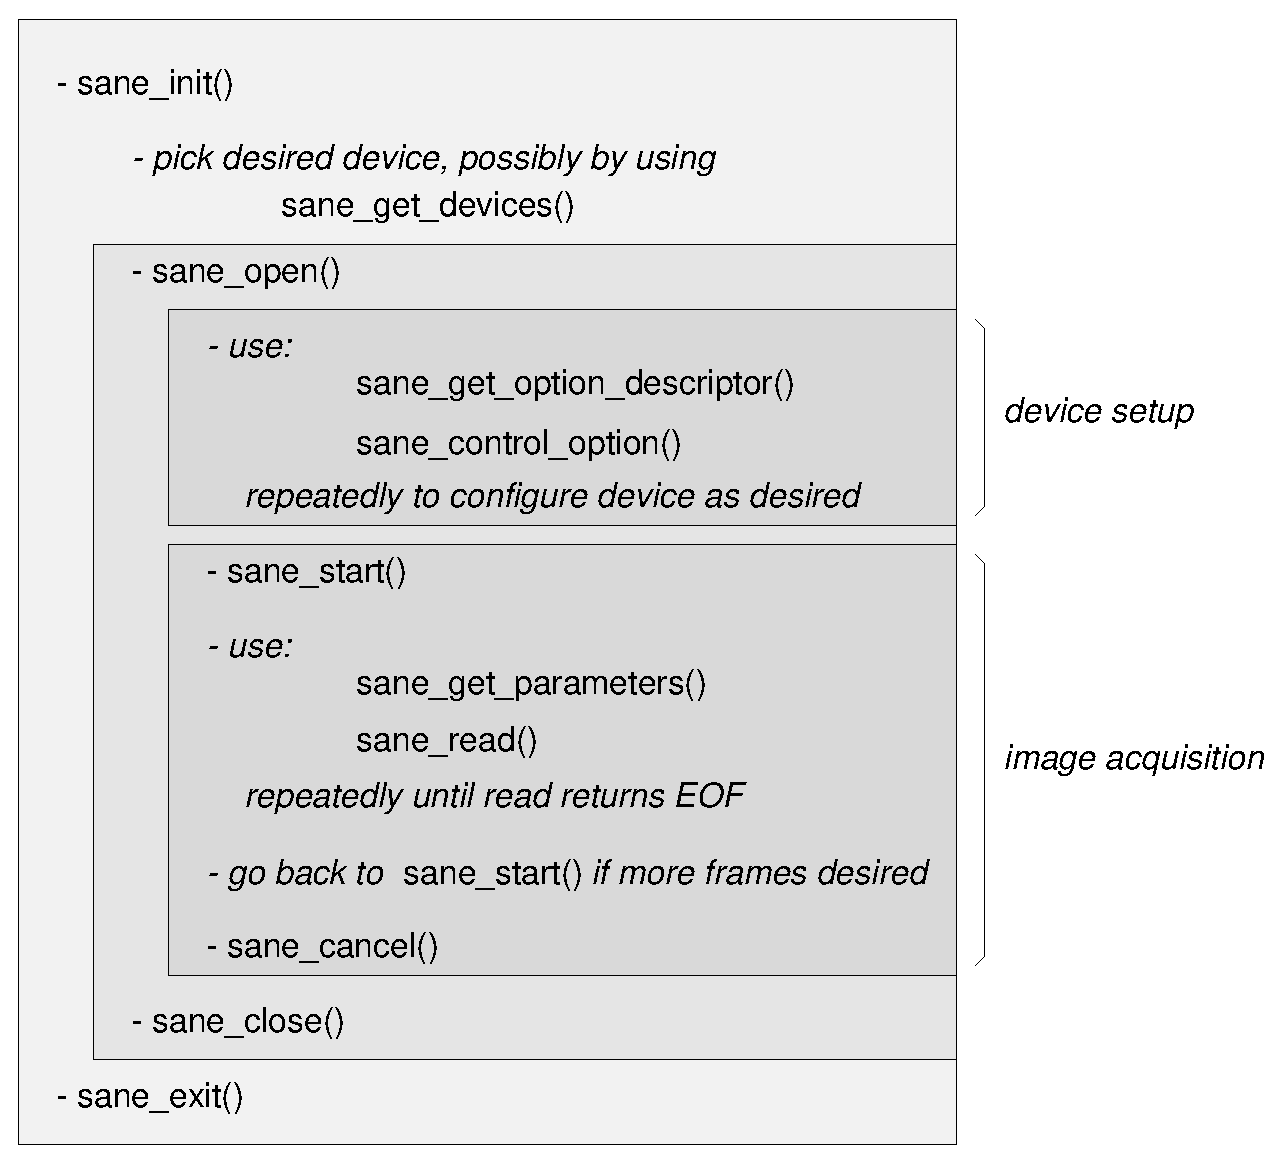
\psfig{file=figs/flow.eps,height=0.5\textheight}
    \caption{Code flow}
    \label{fig:flow}
  \end{center}
\end{figure}

Function \code{sane\_get\_devices()} can be called any time after
\code{sane\_init()} has been called.  It returns the list of the
devices that are known at the time of the call.  This list may change
over time since some devices may be turned on or off or a remote host
may boot or shutdown between different calls.  It should be noted that
this operation may be relatively slow since it requires contacting all
configured devices (some of which may be on remote hosts).  A frontend
may therefore want to provide the ability for a user to directly
select a desired device without requiring a call to this function.

Once a device has been chosen, it is opened using a call to
\code{sane\_open()}.  Multiple devices can be open at any given time.
A SANE backend must not impose artificial constraints on how many
devices can be open at any given time.

An opened device can be setup through the corresponding device handle
using functions \code{sane\_get\_opt\-ion\_desc\-riptor()} and
\code{sane\_control\_option()}.  While setting up a device, obtaining
option descriptors and setting and reading of option values can be
mixed freely.  It is typical for a frontend to read out all available
options at the beginning and then build a dialog (either graphical or
a command-line oriented option list) that allows to control the
available options.  It should be noted that the number of options is
fixed for a given handle.  However, as options are set, other options
may become active or inactive.  Thus, after setting an option, it
maybe necessary to re-read some or all option descriptors.  While
setting up the device, it is also admissible to call
\code{sane\_get\_parameters()} to get an estimate of what the image
parameters will look like once image acquisition begins.

The device handle can be put in blocking or non-blocking mode by a
call to \code{sane\_set\_io\_mode()}.  Devices are required to support
blocking mode (which is the default mode), but support for
non-blocking I/O is strongly encouraged for operating systems such as
UNIX.

After the device is setup properly, image acquisition can be started
by a call to \code{sane\_start()}.  The backend calculates the exact
image parameters at this point.  So future calls to
\code{sane\_get\_parameters()} will return the exact values, rather
than estimates.  Whether the physical image acquisition starts at this
point or during the first call to \code{sane\_read()} is unspecified
by the SANE API.  If non-blocking I/O and/or a select-style interface
is desired, the frontend may attempt to call
\code{sane\_set\_io\_mode()} and/or \code{sane\_get\_select\_fd()} at
this point.  Either of these functions may fail if the backend does
not support the requested operation.

Image data is collected by repeatedly calling \code{sane\_read()}.
Eventually, this function will return an end-of-file status
(\code{SANE\_STATUS\_EOF}).  This indicates the end of the current
frame.  If the frontend expects additional frames (e.g., the
individual channels in of a red/green/blue image or multiple images),
it can call \code{sane\_start()} again.  Once all desired frames have
been acquired, function \code{sane\_cancel()} must be called.  This
operation can also be called at any other time to cancel a pending
operation.  Note that \code{sane\_cancel()} must be called even if the
last read operation returned \code{SANE\_STATUS\_EOF}.

When done using the device, the handle should be closed by a call to
\code{sane\_close()}.  Finally, before exiting the application,
function \code{sane\_exit()} must be called.  It is important not to
forget to call this function since otherwise some resources (e.g.,
temporary files or locks) may remain unclaimed.


\section{Well-Known Options}\index{well-known options}

While most backend options are completely self-describing, there are a
cases where a user interface might want to special-case the handling
of certain options.  For example, the scan area is typically defined
by four options that specify the top-left and bottom-right corners of
the area.  With a graphical user interface, it would be tedious to
force the user to type in these four numbers.  Instead, most such
interfaces will want to present to the user a preview (low-resolution
scan) of the scanner surface and let the user pick the scan area by
dragging a rectangle into the desired position.  For this reason, the
SANE API specifies a small number of option names that have
well-defined meanings.

\subsection{Option Number Count}\index{option count}

Option number 0 has an empty string as its name.  The value of this
option is of type \code{SANE\_TYPE\_INT} and it specifies the total
number of options available for a given device (the count includes
option number 0).  This means that there are two ways of counting the
number of options available: a frontend can either cycle through all
option numbers starting at one until
\code{sane\_get\_option\_descriptor()} returns \code{NULL}, or a
frontend can directly read out the value of option number 0.

\subsection{Scan Resolution Option}\index{scan resolution}\index{resolution option}

Option \code{resolution} is used to select the resolution at which an
image should be acquired.  The type of this option is either
\code{SANE\_TYPE\_INT} or \code{SANE\_TYPE\_FIXED}.  The unit is
\code{SANE\_UNIT\_DPI} (dots/inch).

This option is not mandatory, but if a backend does support it, it
must implement it in a manner consistent with the above definition.

\subsection{Preview Mode Option}\index{preview mode}

The boolean option \code{preview} is used by a frontend to inform the
backend when image acquisition should be optimized for speed, rather
than quality (``preview mode'').  When set to \code{SANE\_TRUE},
preview mode is in effect, when set to \code{SANE\_FALSE} image
acquisition should proceed in normal quality mode.  The setting of
this option \emph{must not\/} affect any other option.  That is, as
far as the other options are concerned, the preview mode is completely
side effect free.  A backend can assume that the frontend will take
care of appropriately setting the scan resolution for preview mode
(through option \code{resolution}).  A backend is free to override the
\code{resolution} value with its own choice for preview mode, but it
is advised to leave this choice to the frontend wherever possible.

This option is not mandatory, but if a backend does support it, it
must implement it in a manner consistent with the above definition.

\subsection{Scan Area Options}\index{scan area options}

The four most important well-known options are the ones that define
the scan area.  The scan area is defined by two points (x/y coordinate
pairs) that specify the top-left and the bottom-right corners.  This
is illustrated in Figure~\ref{fig:area}.  Note that the origin of the
coordinate system is at the top-left corner of the scan surface as
seen by the sensor (which typically is a mirror image of the scan
surface seen by the user).  For this reason, the top-left corner is
the corner for which the abscissa and ordinate values are
simultaneously the {\em smallest} and the bottom-right corner is the
corner for which the abscissa and ordinate values are simulatenously
the {\em largest}.  If this coordinate system is not natural for a
given device, it is the job of the backend to perform the necessary
conversions.
\begin{figure}[tbp]
  \begin{center}
    \leavevmode
    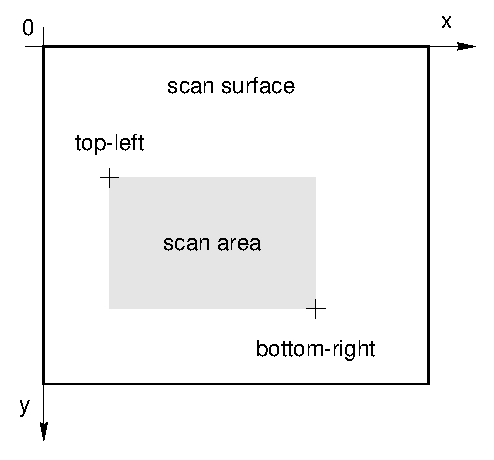
\psfig{file=figs/area.eps,height=0.3\textheight}
    \caption{Scan area options}
    \label{fig:area}
  \end{center}
\end{figure}

The names of the four options that define the scan area are given in
the table below:
\begin{center}
\begin{tabular}{ll}
{\bf Name} & {\bf Description} \\
\code{\defn{tl-x}} & Top-left $x$ coordinate value \\
\code{\defn{tl-y}} & Top-left $y$ coordinate value \\
\code{\defn{br-x}} & Bottom-right $x$ coordinate value \\
\code{\defn{br-y}} & Bottom-right $y$ coordinate value \\
\end{tabular}
\end{center}
There are several rules that should be followed by front and backends
regarding these options:
\begin{itemize}

\item Backends must attach a unit of either pixels
  (\code{SANE\_UNIT\_PIXEL}) or millimeters (\code{SANE\_UNIT\_MM}) to
  these options.  The unit of all four options must be identical.

\item Whenever meaningful, a backend should attach a range or a
  word-list constraint to these options.

\item A frontend can determine the size of the scan surface by first
  checking that the options have range constraints associated.  If a
  range or word-list constraints exist, the frontend can take the
  minimum and maximum values of one of the x and y option
  range-constraints to determine the scan surface size.

\item A frontend must work properly with any or all of these options
  missing.
  
\end{itemize}

\chapter{Network Protocol}\label{chap:net}

The SANE interface has been designed to facilitate network access to
image acquisition devices.  In particular, most SANE implementations
are expected to support a network backend (net client) and a
corresponding network daemon (net server) that allows accessing image
acquisition devices through a network connection.  Network access is
useful in several situations:
\begin{itemize}

\item To provide controlled access to resources that are inaccessible
  to a regular user.  For example, a user may want to access a device
  on a host where she has no account on.  With the network protocol,
  it is possible to allow certain users to access scanners without
  giving them full access to the system.

  Controlling access through the network daemon can be useful even in
  the local case: for example, certain backends may require root
  privileges to access a device.  Rather than installing each frontend
  as setuid-root, a system administrator could instead install the
  SANE network daemon as setuid-root.  This enables regular users to
  access the privileged device through the SANE daemon (which,
  presumably, supports a more fine-grained access control mechanism
  than the simple setuid approach).  This has the added benefit that
  the system administrator only needs to trust the SANE daemon, not
  each and every frontend that may need access to the privileged
  device.

\item Network access provides a sense of ubiquity of the available
  image acquisition devices.  For example, in a local area network
  environment, this allows a user to log onto any machine and have
  convenient access to any resource available to any machine on the
  network (subject to permission constraints).

\item For devices that do not require physical access when used (e.g.,
  video cameras), network access allows a user to control and use
  these devices without being in physical proximity.  Indeed, if such
  devices are connected to the Internet, access from any place in the
  world is possible.

\end{itemize}

The network protocol described in this chapter has been design with
the following goals in mind:
\begin{enumerate}

\item Image transmission should be efficient (have low encoding
  overhead).

\item Accessing option descriptors on the client side must be
  efficient (since this is a very common operation).

\item Other operations, such as setting or inquiring the value of an
  option are less performance critical since they typically require
  explicit user action.

\item The network protocol should be simple and easy to implement on
  any host architecture and any programming language.

\end{enumerate}
The SANE protocol can be run across any transport protocol that
provides reliable data delivery.  While SANE does not specify a
specific transport protocol, it is expected that TCP/IP will be among
the most commonly used protocols.

\section{Data Type Encoding}

\subsection{Primitive Data Types}

The four primitive types of the SANE standard are encoded as follows:
\begin{description}

\item[\code{\defn{SANE\_Byte}}:] A byte is encoded as an 8 bit value.
  Since the transport protocol is assumed to be byte-orientd, the bit
  order is irrelevant.

\item[\code{\defn{SANE\_Word}}:] A word is encoded as 4 bytes (32
  bits).  The bytes are ordered from most-significant to
  least-significant byte (big-endian byte-order).

\item[\code{\defn{SANE\_Char}}:] A character is currently encoded as an 8-bit
  ISO LATIN-1 value.  An extension to support wider character sets (16 or 32
  bits) is planned for the future, but not supported at this point.

\item[\code{\defn{SANE\_String}}:] A string pointer is encoded as a
  \code{SANE\_Char} array.  The trailing NUL byte is considered part
  of the array and a \code{NULL} pointer is encoded as a zero-length
  array.
  
\item[\code{\defn{SANE\_Handle}}:] A handle is encoded like a word.
  The network backend needs to take care of converting these integer
  values to the opaque pointer values that are presented to the user
  of the network backend.  Similarly, the SANE daemon needs to take
  care of converting the opaque pointer values it receives from its
  backends into 32-bit integers suitable for use for network encoding.

\item[{\em\defn{enumeration types}}:] Enumeration types are encoded
  like words.

\end{description}

\subsection{Type Constructors}

Closely following the type constructors of the C language, the SANE network
protocol supports the following four constructors:
\begin{description}

\item[{\em\defn{pointer}}:] A pointer is encoded by a word that indicates
  whether the pointer is a NULL-pointer which is then followed by the
  value that the pointer points to (in the case of a non-NULL pointer;
  in the case of a NULL pointer, no bytes are encoded for the pointer
  value).

\item[{\em\defn{array}}:] An array is encoded by a word that indicates
  the length of the array followed by the values of the elements in
  the array.  The length may be zero in which case no bytes are
  encoded for the element values.

\item[{\em\defn{structure}}:] A structure is encoded by simply encoding the
  structure members in the order in which they appear in the
  corresponding C type declaration.

\item[{\em\defn{union}}:] A union must always be accompanied by a tag
  value that indicates which of the union members is the currently the
  active one.  For this reason, the union itself is encoded simply by
  encoding the value of the currently active member.

\end{description}

Note that for type constructors, the pointer, element, or member
values themselves may have a constructed type.  Thus, the above rules
should be applied recursively until a sequence of primitive types has
been found.

Also SANE had no need for encoding of circular structures.  This
greatly simplifies the network protocol.

\section{Remote Procedure Call Requests}

The SANE network protocol is a client/server-style remote procedure
call (RPC) protocol.  This means that all activity is initiated by the
client side (the network backend)---a server is restricted to
answering request by the client.

\subsection{\code{\defn{SANE\_NET\_INIT}}}

This RPC establishes a connection to a particular SANE network daemon.
It must be the first call in a SANE network session.  The parameter
and reply arguments for this call are shown in the table below:
\begin{center}
\begin{tabular}{ll}
  {\bf request:} & {\bf reply:} \\
  \code{SANE\_Word version\_code} & \code{SANE\_Word status} \\
  \code{SANE\_String user\_name}   & \code{SANE\_Word version\_code} \\
\end{tabular}
\end{center}
The \code{version\_code} argument in the request is the SANE
version-code of the network backend that is contacting the network
daemon (see Section~\ref{sec:saneversioncode}).  The
``build-revision'' in the version code is used to hold the network
protocol version.  The SANE network daemon receiving such a request
must make sure that the network protocol version corresponds to a
supported version since otherwise the encoding of the network stream
may be incompatible (even though the SANE interface itself may be
compatible).  The \code{user\_name} argument is the name of the user
on whose behalf this call is being performed.  If the network backend
cannot determine a user-name, it passes a \code{NULL} pointer for this
argument.  No trust should be placed in the authenticity of this
user-name.  The intent of this string is to provide more convenience
to the user.  E.g., it could be used as the default-user name in
subsequent authentication calls.

In the reply, \code{status} indicates the completion status.  If the
value is anything other than \code{SANE\_STA\-TUS\_SUCCESS}, the
remainder of the reply has undefined values.\footnote{The sane network
  daemon should be careful not to leak information in the undefined
  portion of the reply.} The \code{version\_code} argument returns the
SANE version-code that the network daemon supports.  See the comments
in the previous paragraph on the meaning of the build-revision in this
version code.

\subsection{\code{\defn{SANE\_NET\_GET\_DEVICES}}}

This RPC is used to obtain the list of devices accessible by the SANE
daemon.
\begin{center}
\begin{tabular}{ll}
  {\bf request:} & {\bf reply:} \\
  \code{void} & \code{SANE\_Word status} \\
              & \code{SANE\_Device ***device\_list} \\
\end{tabular}
\end{center}
There are no arguments in the request for this call.

In the reply, \code{status} indicates the completion status.  If the
value is anything other than \code{SANE\_STA\-TUS\_SUCCESS}, the
remainder of the reply has undefined values.  The \code{device\_list}
argument is a pointer to a \code{NULL}-terminated array of
\code{SANE\_Device} pointers.

\subsection{\code{\defn{SANE\_NET\_OPEN}}}

This RPC is used to open a connection to a remote SANE device.
\begin{center}
\begin{tabular}{ll}
  {\bf request:} & {\bf reply:} \\
  \code{SANE\_String device\_name} & \code{SANE\_Word status} \\
                                   & \code{SANE\_Word handle} \\
                                   & \code{SANE\_String resource} \\
\end{tabular}
\end{center}
The \code{device\_name} argument specifies the name of the device to
open.

In the reply, \code{status} indicates the completion status.  If the
value is anything other than \code{SANE\_STA\-TUS\_SUCCESS}, the
remainder of the reply has undefined values.  The \code{handle}
argument specifies the device handle that uniquely identifies the
connection.  The \code{resource} argument is used to request
authentication.  If it has a non-\code{NULL} value, the network
backend should authenticate the specified resource and then retry this
operation (see Section~\ref{sec:authorization} for details on how to
authorize a resource).

\subsection{\code{\defn{SANE\_NET\_CLOSE}}}

This RPC is used to close a connection to a remote SANE device.
\begin{center}
\begin{tabular}{ll}
  {\bf request:} & {\bf reply:} \\
  \code{SANE\_Word handle} & \code{SANE\_Word dummy} \\
\end{tabular}
\end{center}
The \code{handle} argument identifies the connection that should be
closed.

In the reply, the \code{dummy} argument is unused.  Its purpose is to
ensure proper synchronization (without it, a net client would not be
able to determine when the RPC has completed).

\subsection{\code{\defn{SANE\_NET\_GET\_OPTION\_DESCRIPTORS}}}

This RPC is used to obtain {\em all\/} the option descriptors for a
remote SANE device.
\begin{center}
\begin{tabular}{ll}
  {\bf request:} & {\bf reply:} \\
  \code{SANE\_Word handle} & \code{Option\_Descriptor\_Array odesc} \\
\end{tabular}
\end{center}
The \code{handle} argument identifies the remote device whose option
descriptors should be obtained.

In the reply, the \code{odesc} argument is used to return the array of
option descriptors.  The option descriptor array has the following
structure:
\begin{quote}\index{Option\_Descriptor\_Array}
\begin{verbatim}
struct Option_Descriptor_Array
  {
    SANE_Word num_options;
    SANE_Option_Descriptor **desc;
  };
\end{verbatim}
\end{quote}


\subsection{\code{\defn{SANE\_NET\_CONTROL\_OPTION}}}

This RPC is used to control (inquire, set, or set to automatic) a
specific option of a remote SANE device.
\begin{center}
\begin{tabular}{ll}
  {\bf request:} & {\bf reply:} \\
  \code{SANE\_Word handle}      & \code{SANE\_Status status} \\
  \code{SANE\_Word option}      & \code{SANE\_Word info} \\
  \code{SANE\_Word action}      & \code{SANE\_Word value\_type} \\
  \code{SANE\_Word value\_type} & \code{SANE\_Word value\_size} \\
  \code{SANE\_Word value\_size} & \code{void *value} \\
  \code{void *value}            & \code{SANE\_String *resource} \\
\end{tabular}
\end{center}
The \code{handle} argument identifies the remote device whose option
should be controlled.  Argument \code{option} is the number (index) of
the option that should be controlled.  Argument \code{action}
specifies what action should be taken (get, set, or set automatic).
Argument \code{value\_type} specifies the type of the option value
(must be one of \code{SANE\_TYPE\_BOOL}, \code{SANE\_TYPE\_INT},
\code{SANE\_TYPE\_FIXED}, \code{SANE\_TYPE\_STR\-ING},
\code{SANE\_TYPE\_BUTTON}).  Argument \code{value\_size} specifies
the size of the option value in number of bytes (see
Section~\ref{sec:valuesize} for the precise meaning of this value).
Finally, argument \code{value} is a pointer to the option value.  It
must be a writeable area that is at least \code{value\_size} bytes
large. (Note that this area must be writable even if the action is to
set the option value.  This is because the backend may not be able to
set the exact option value, in which case the option value is used to
return the next best value that the backend has chosen.)

In the reply, argument \code{resource} is set to the name of the
resource that must be authorized before this call can be retried.  If
this value is non-\code{NULL}, all other arguments have undefined
values (see Section~\ref{sec:authorization} for details on how to
authorize a resource).  Argument \code{status} indicates the
completion status.  If the value is anything other than
\code{SANE\_STA\-TUS\_SUCCESS}, the remainder of the reply has undefined
values.  The \code{info} argument returns the information on how well
the backend was able to satisfy the request.  For details, see the
description of the corresponding argument in
Section~\ref{sec:control}.  Arguments \code{value\_type} and
\code{value\_size} have the same values as the arguments by the same
name in corresponding request.  The values are repeated here to ensure
that both the request and the reply are self-contained (i.e., they can
be encoded and decoded independently).  Argument \code{value} is holds
the value of the option that has become effective as a result of this
RPC.


\subsection{\code{\defn{SANE\_NET\_GET\_PARAMETERS}}}

This RPC is used to obtain the scan parameters of a remote SANE
device.
\begin{center}
\begin{tabular}{ll}
  {\bf request:} & {\bf reply:} \\
  \code{SANE\_Word handle} & \code{SANE\_Status status} \\
                           & \code{SANE\_Parameters params} \\
\end{tabular}
\end{center}
The \code{handle} argument identifies the connection to the remote
device whose scan parameters should be returned.

In the reply, \code{status} indicates the completion status.  If the
value is anything other than \code{SANE\_STA\-TUS\_SUC\-CESS}, the
remainder of the reply has undefined values.  The argument
\code{params} is used to return the scan parameters.

\subsection{\code{\defn{SANE\_NET\_START}}}

This RPC is used to start image acquisition (scanning).
\begin{center}
\begin{tabular}{ll}
  {\bf request:} & {\bf reply:} \\
  \code{SANE\_Word handle} & \code{SANE\_Status status} \\
                           & \code{SANE\_Word port} \\
                           & \code{SANE\_Word byte\_order} \\
                           & \code{SANE\_String resource} \\
\end{tabular}
\end{center}
The \code{handle} argument identifies the connection to the remote
device from which the image should be acquired.

In the reply, argument \code{resource} is set to the name of the
resource that must be authorized before this call can be retried.  If
this value is non-\code{NULL}, all other arguments have undefined
values (see Section~\ref{sec:authorization} for details on how to
authorize a resource).  Argument, \code{status} indicates the
completion status.  If the value is anything other than
\code{SANE\_STA\-TUS\_SUCCESS}, the remainder of the reply has
undefined values.  The argument \code{port} returns the port number
from which the image data will be available.  To read the image data,
a network client must connect to the remote host at the indicated port
number.  Through this port, the image data is transmitted as a
sequence of data records.  Each record starts with the data length in
bytes.  The data length is transmitted as a sequence of four bytes.
These bytes should be interpreted as an unsigned integer in big-endian
format.  The four length bytes are followed by the number of data
bytes indicated by the length.  Except for byte-order, the data is in
the same format as defined for \code{sane\_read()}.  Since some
records may contain no data at all, a length value of zero is
perfectly valid.  The special length value of \code{0xffffffff} is
used to indicate the end of the data stream.  That is, after receiving
a record length of \code{0xffffffff}, the network client should close
the data connection and stop reading data.

Argument \code{byte\_order} specifies the byte-order of the image
data.  A value of 0x1234 indicates little-endian format, a value of
0x4321 indicates big-endian format.  All other values are presently
undefined and reserved for future enhancements of this protocol.  The
intent is that a network server sends data in its own byte-order and
the client is responsible for adjusting the byte-order, if necessary.
This approach causes no unnecessary overheads in the case where the
server and client byte-order match and puts the extra burden on the
client side when there is a byte-order mismatch.  Putting the burden
on the client-side improves the scalability properties of this
protocol.

\subsection{\code{\defn{SANE\_NET\_CANCEL}}}

This RPC is used to cancel the current operation of a remote SANE
device.
\begin{center}
\begin{tabular}{ll}
  {\bf request:} & {\bf reply:} \\
  \code{SANE\_Word handle} & \code{SANE\_Word dummy} \\
\end{tabular}
\end{center}
The \code{handle} argument identifies the connection whose operation
should be cancelled.

In the reply, the \code{dummy} argument is unused.  Its purpose is to
ensure proper synchronization (without it, a net client would not be
able to determine when the RPC has completed).

\subsection{\code{\defn{SANE\_NET\_AUTHORIZE}}}\label{sec:authorization}
\index{network authorization}

This RPC is used to pass authorization data from the net client to the
net server.
\begin{center}
\begin{tabular}{ll}
  {\bf request:} & {\bf reply:} \\
  \code{SANE\_String resource} & \code{SANE\_Word dummy} \\
  \code{SANE\_String username} & \\
  \code{SANE\_String password} & \\
\end{tabular}
\end{center}
The \code{resource} argument specifies the name of the resource to be
authorized.  This argument should be set to the string returned in the
\code{resource} argument of the RPC reply that required this
authorization call.  The \code{username} and \code{password} are the
name of the user that is accessing the resource and the password for
the specified resource/user pair.

Since the password is not encrypted during network transmission, it is
recommended to use the following extension:

If the server adds the string `\code{\$MD5\$}' to the resource-name followed
by a random string not longer then 128 bytes, the client may answer with the
MD5 digest of the concatenation of the password and the random string. To
differentiate between the MD5 digest and a strange password the client prepends
the MD5 digest with the string `\code{\$MD5\$}'.

In the reply, \code{dummy} is completely unused.  Note that there is
no direct failure indication.  This is unnecessary since a net client
will retry the RPC that resulted in the authorization request until
that call succeeds (or until the request is cancelled). The RPC that resulted
in the authorization request continues after the reply from the client and may
fail with \code{SANE\_STATUS\_ACCESS\_DENIED}.


\subsection{\code{\defn{SANE\_NET\_EXIT}}}

This RPC is used to disconnect a net client from a net server.  There
are no request or reply arguments in this call.  As a result of this
call, the connection between the client and the server that was
established by the \code{SANE\_NET\_INIT} call will be closed.

% Local Variables: 
% mode: latex
% TeX-master: "sane.tex"
% End: 


\chapter{Contact Information}\label{chap:contact}

The SANE standard is discussed and evolved via a mailing list.
Anybody with email access to the Internet can automatically join and
leave the discussion group by sending mail to the following address.
\begin{quote}\index{mailing list}
\begin{verbatim}
majordomo@mostang.com
\end{verbatim}
\end{quote}
To subscribe, send a mail with the body ``\verb|subscribe sane-devel|'' to the
above address.

A complete list of commands supported can be obtained by sending a
mail with a subject of ``\code{help}'' to the above address.  The
mailing list is archived and available through the SANE home page at
URL:
\begin{quote}
\url{http://www.mostang.com/sane/}
\end{quote}

\newpage
\documentclass[11pt,DVIps]{report}

\usepackage{times,epsfig,changebar,html}

\setlength{\parindent}{0pt}
\setlength{\parskip}{1.5ex plus 0.5ex minus 0.5ex}
\setlength{\textwidth}{6.5in}
\setlength{\textheight}{8.5in}
\setlength{\marginparwidth}{0pt}
\setlength{\oddsidemargin}{0pt}
\setlength{\evensidemargin}{0pt}
\setlength{\marginparsep}{0pt}
\addtolength{\topmargin}{-0.75in}

\title{\huge SANE Standard Version 1.02}
\author{}
\date{February 19, 2002} 

\makeindex

\begin{document}

\newcommand{\filename}[1]{{\tt #1}}
\newcommand{\code}[1]{{\tt #1}}
\newcommand{\var}[1]{{\it #1}}
\newcommand{\defn}[1]{#1\index{#1}}

\begin{latexonly}
  \setcounter{changebargrey}{0}   % black change bars
\end{latexonly}

\maketitle
\tableofcontents
\listoffigures
\listoftables


\chapter{Preface}

The SANE standard is being developed by a group of free-software
developers.  The process is open to the public and comments as well as
suggestions for improvements are welcome.  Information on how to join
the SANE development process can be found in Chapter
\ref{chap:contact}.

The SANE standard is intended to streamline software development by
providing a standard application programming interface to access
raster scanner hardware.  This should reduce the number of different
driver implementations, thereby reducing the need for reimplementing
similar code.


\section{About This Document}

This document is intended for developers who are creating either an
application that requires access to raster scanner hardware and for
developers who are implementing a SANE driver.  It does not cover
specific implementations of SANE components.  Its sole purpose is to
describe and define the SANE application interface that will enable
any application on any platform to interoperate with any SANE backend
for that platform.

The remainder of this document is organized as follows.
Chapter~\ref{chap:intro} provides introductional material.
Chapter~\ref{chap:environ} presents the environment SANE is designed
for.  Chapter~\ref{chap:api} details the SANE Application Programmer
Interface.  Chapter~\ref{chap:net} specifies the network protocol that
can be used to implement the SANE API in a network transparent
fashion.  Finally, Chapter~\ref{chap:contact} gives information on how
to join the SANE development process.

\subsection{Typographic Conventions}

Changes since the last revision of this document are highlighted
like this:

% \begin{changebar}
%   Paragraphs that changed since the last revision of the documention
%   are marked like this paragraph.
% \end{changebar}

\chapter{Introduction}\label{chap:intro}

SANE is an application programming interface (API) that provides
standardized access to any raster image scanner hardware.  The
standardized interface allows to write just one driver for each
scanner device instead of one driver for each scanner and application.
The reduction in the number of required drivers provides significant
savings in development time.  More importantly, SANE raises the level
at which applications can work.  As such, it will enable applications
that were previously unheard of in the UNIX world.  While SANE is
primarily targeted at a UNIX environment, the standard has been
carefully designed to make it possible to implement the API on
virtually any hardware or operating system.

SANE is an acronym for ``Scanner Access Now Easy.''  Also, the hope is
that SANE is sane in the sense that it will allow easy implementation
of the API while accommodating all features required by today's
scanner hardware and applications.  Specifically, SANE should be broad
enough to accommodate devices such as scanners, digital still and
video cameras, as well as virtual devices like image file filters.

\section{Terminology}

An application that uses the SANE interface is called a SANE {\em
  frontend}.  A driver that implements the SANE interface is called a
SANE {\em backend}.  A {\em meta backend\/} provides some means to
manage one or more other backends.


\chapter{The SANE Environment}\label{chap:environ}

SANE is defined as a C-callable library interface.  Accessing a raster
scanner device typically consists of two phases: first, various
controls of the scanner need to be setup or queried.  In the second
phase, one or more images are acquired.

Since the device controls are widely different from device to device,
SANE provides a generic interface that makes it easy for a frontend to
give a user access to all controls without having to understand each
and every device control.  The design principle used here is to
abstract each device control into a SANE {\em option\/}.  An option is
a self-describing name/value pair.  For example, the brightness
control of a camera might be represented by an option called
\code{brightness} whose value is an integer in the range from 0 to
255.

With self-describing options, a backend need not be concerned with
{\em presentation\/} issues: the backend simply provides a list of
options that describe all the controls available in the device.
Similarly, there are benefits to the frontend: it need not be
concerned with the {\em meaning\/} of each option.  It simply provides
means to present and alter the options defined by the backend.


\section{Attaching to a SANE backend}

The process through which a SANE frontend connects to a backend is
platform dependent.  Several possibilities exist:
\begin{itemize}

\item {\bf Static linking:} A SANE backend may be linked directly into
  a frontend.  While the simplest method of attaching to a backend, it
  is somewhat limited in functionality since the available devices is
  limited to the ones for which support has been linked in when the
  frontend was built.  But even so static linking can be quite useful,
  particularly when combined with a backend that can access scanners
  via a network.  Also, it is possible to support multiple backends
  simultaneously by implementing a meta backend that manages several
  backends that have been compiled in such a manner that they export
  unique function names.  For example, a backend called \code{be}
  would normally export a function called \code{sane\_read()}.  If
  each backend would provide such a function, static linking would
  fail due to multiple conflicting definitions of the same symbol.
  This can be resolved by having backend \code{be} include a
  header file that has lines of the form:
  \begin{quote}
\begin{verbatim}
#define sane_read be_sane_read
\end{verbatim}
  \end{quote}
  With definitions of this kind, backend \code{be} will export
  function name \code{be\_sane\_read()}.  Thus, all backends will
  export unique names.  As long as a meta backend knows about these
  names, it is possible to combine several backends at link time and
  select and use them dynamically at runtime.

\item {\bf Dynamic linking:} A simpler yet more powerful way to
  support multiple backends is to exploit dynamic linking on platforms
  that support it.  In this case, a frontend is linked against a
  shared library that implements any SANE backend.  Since each
  dynamically linked backend exports the same set of global symbols
  (all starting with the prefix \code{sane\_}), the dynamic library
  that gets loaded at runtime does not necessarily have to be the same
  one as one the frontend got linked against.  In other words, it is
  possible to switch the backend by installing the appropriate backend
  dynamic library.

  More importantly, dynamic linking makes it easy to implement a meta
  backend that loads other backends {\em on demand}.  This is a
  powerful mechanism since it allows adding new backends merely by
  installing a shared library and updating a configuration file.

\item {\bf Network connection:} Arguably the ultimate way to attach to
  a scanner is by using the network to connect to a backend on a
  remote machine.  This makes it possible to scan images from any host
  in the universe, as long as there is a network connection to that
  host and provided the user is permitted to access that scanner.

\end{itemize}

\begin{figure}[htbp]
  \begin{center}
    \leavevmode
    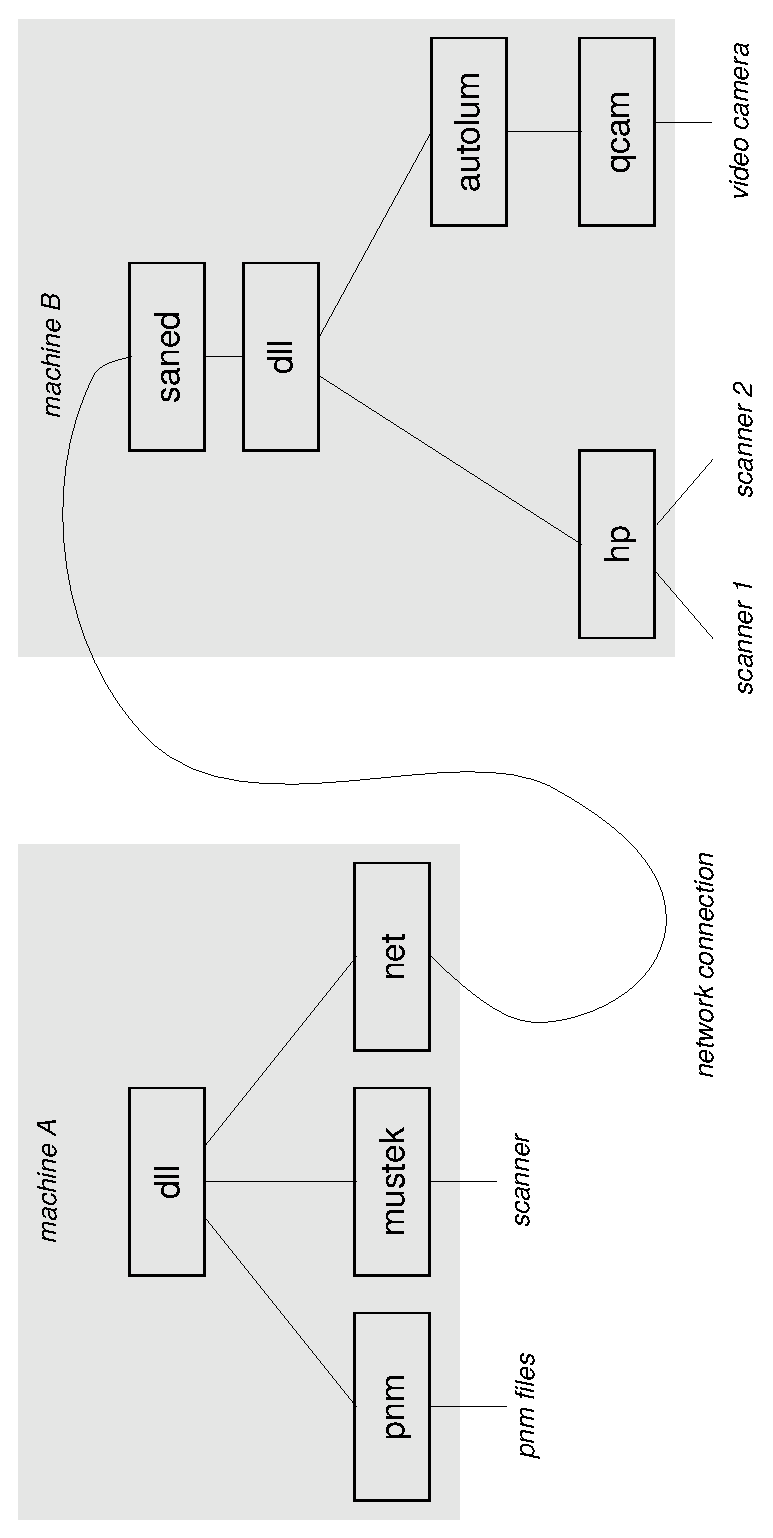
\psfig{file=figs/hierarchy.eps,angle=270,width=\textwidth}
    \caption{Example SANE Hiearchy}
    \label{fig:hierarchy}
  \end{center}
\end{figure}

The above discussion lists just a few ways for frontends to attach to
a backend.  It is of course possible to combine these solutions to
provide an entire hierarchy of SANE backends.  Such a hierarchy is
depicted in Figure~\ref{fig:hierarchy}.  The figure shows that machine
A uses a dynamic-linking based meta backend called \code{dll} to
access the backends called \code{pnm}, \code{mustek}, and \code{net}.
The first two are real backends, whereas the last one is a meta
backend that provides network transparent access to remote scanners.
In the figure, machine B provides non-local access to its scanners
through the SANE frontend called \code{saned}.  The \code{saned} in
turn has access to the \code{hp} and \code{autolum} backends through
another instance of the \code{dll} backend.  The \code{autolum} meta
backend is used to automatically adjust the luminance (brightness) of
the image data acquired by the camera backend called \code{qcam}.

Note that a meta backend really is both a frontend and a backend at
the same time.  It is a frontend from the viewpoint of the backends
that it manages and a backend from the viewpoint of the frontends that
access it.  The name ``meta backend'' was chosen primarily because the
SANE standard describes the interface from the viewpoint of a (real)
frontend.


\section{Image Data Format}\label{sec:imageformat}\index{image data format}

Arguably the most important aspect of an image acquisition system is
how images are represented.  The SANE approach is to define a simple
yet powerful representation that is sufficient for vast majority of
applications and devices.  While the representation is simple, the
interface has been defined carefully to allow extending it in the
future without breaking backwards compatibility.  Thus, it will be
possible to accommodate future applications or devices that were not
anticipated at the time this standard was created.

A SANE image is a rectangular area.  The rectangular area is
subdivided into a number of rows and columns.  At the intersection of
each row and column is a quadratic pixel.  A pixel consists of one or
more sample values.  Each sample value represents one channel (e.g.,
the red channel).  Each sample value has a certain bit depth.  The bit
depth is fixed for the entire image and can be as small as one bit.
Valid bit depths are 1, 8, or 16 bits per sample.  If a device's
natural bit depth is something else, it is up to the driver to scale
the sample values appropriately (e.g., a 4 bit sample could be scaled
by a factor of four to represent a sample value of depth 8).

\subsection{Image Transmission}

The SANE API transmits an image as a sequence of frames.  Each frame
covers the same rectangular area as the entire image, but may contain
only a subset of the channels in the final image.  For example, a
red/green/blue image could either be transmitted as a single frame
that contains the sample values for all three channels or it could be
transmitted as a sequence of three frames: the first frame containing
the red channel, the second the green channel, and the third the blue
channel.

Conceptually, each frame is transmitted a byte at a time.  Each byte
may contain 8 sample values (for an image bit depth of 1), one full
sample value (for an image bit depth of 8), or a partial sample value
(for an image bit depth of 16 or bigger).  In the latter case, the
bytes of each sample value are transmitted in the machine's native
byte order.
\begin{quote}
  \begin{center}
    {\bf Backend Implementation Note}
  \end{center}
  A network-based meta backend will have to ensure that the byte order
  in image data is adjusted appropriately if necessary.  For example,
  when the meta backend attaches to the server proxy, the proxy may
  inform the backend of the server's byte order.  The backend can then
  apply the adjustment if necessary.  In essence, this implements a
  ``receiver-makes-right'' approach.
\end{quote}

\begin{figure}[htbp]
  \begin{center}
    \leavevmode
    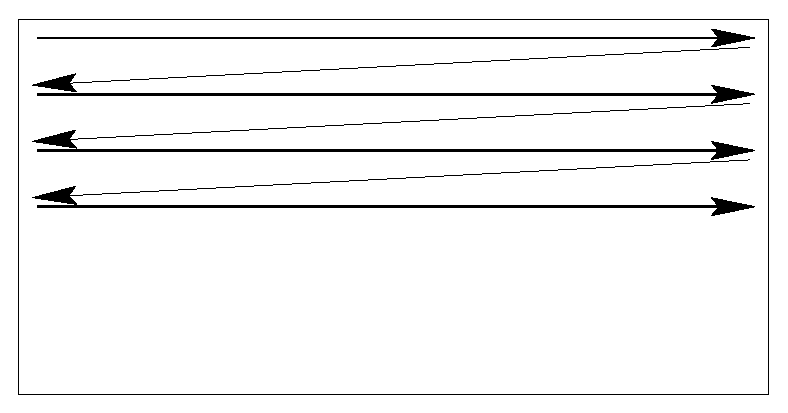
\psfig{file=figs/xfer.eps,width=0.5\textwidth}
    \caption{Transfer order of image data bytes}
    \label{fig:xfer}
  \end{center}
\end{figure}

The order in which the sample values in a frame are transmitted is
illustrated in Figure~\ref{fig:xfer}.  As can be seen, the values are
transmitted row by row and each row is transmitted from left-most to
right-most column.  The left-to-right, top-to-bottom transmission
order applies when the image is viewed in its normal orientation (as
it would be displayed on a screen, for example).

If a frame contains multiple channels, then the channels are
transmitted in an interleaved fashion.  Figure~\ref{fig:pixels}
illustrates this for the case where a frame contains a complete
red/green/blue image with a bit-depth of 8.  For a bit depth of 1,
each byte contains 8 sample values of a {\em single\/} channel.  In
other words, a bit depth 1 frame is transmitted in a byte interleaved
fashion.

\begin{figure}[htbp]
  \begin{center}
    \leavevmode
    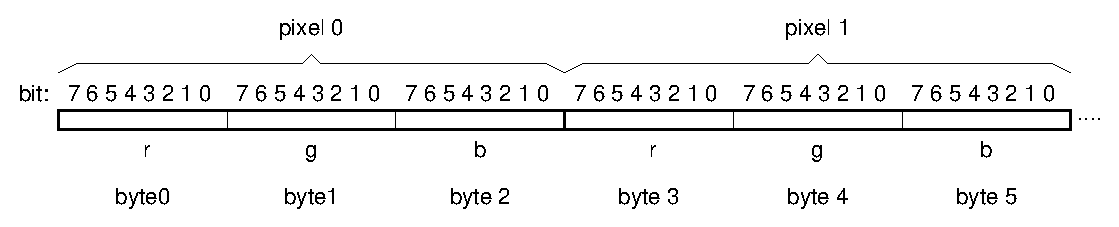
\psfig{file=figs/image-data.eps,width=0.8\textwidth}
    \caption{Bit and byte order or image data}
    \label{fig:pixels}
  \end{center}
\end{figure}

When transmitting an image frame by frame, the frontend needs to know
what part of the image a frame represents (and how many frames it
should expect).  For that purpose, the SANE API tags every frame with
a type.  This version of the SANE standard supports the following
frame types:
\begin{quote}
\begin{description}

\item[\code{\defn{SANE\_FRAME\_GRAY}}:] The frame contains a single
  channel of data that represents sample values from a spectral band
  that covers the human visual range.  The image consists of this
  frame only.

\item[\code{\defn{SANE\_FRAME\_RGB}}:] The frame contains three
  channels of data that represent sample values from the red, green,
  and blue spectral bands.  The sample values are interleaved in the
  order red, green, and blue.  The image consists of this frame only.

\item[\code{\defn{SANE\_FRAME\_RED}}:] The frame contains one channel
  of data that represents sample values from the red spectral band.
  The complete image consists of three frames:
  \code{SANE\_\-FRA\-ME\_RED}, \code{SANE\_FRAME\_GREEN}, and
  \code{SANE\_FRAME\_BLUE}.  The order in which the frames are
  transmitted chosen by the backend.

\item[\code{\defn{SANE\_FRAME\_GREEN}}:] The frame contains one
  channel of data that represents sample values from the green
  spectral band.  The complete image consists of three frames:
  \code{SANE\_\-FRA\-ME\_RED}, \code{SANE\_FRAME\_GREEN}, and
  \code{SANE\_FRAME\_BLUE}.  The order in which the frames are
  transmitted chosen by the backend.

\item[\code{\defn{SANE\_FRAME\_BLUE}}:] The frame contains one channel
  of data that represents sample values from the blue spectral band.
  The complete image consists of three frames:
  \code{SANE\_\-FRA\-ME\_RED}, \code{SANE\_FRAME\_GREEN}, and
  \code{SANE\_FRAME\_BLUE}.  The order in which the frames are
  transmitted chosen by the backend.

\end{description}
\end{quote}

In frames of type SANE\_FRAME\_GRAY, when the bit depth is 1 there are
only two sample values possible, 1 represents minimum intensity
(black) and 0 represents maximum intensity (white).  For all other bit
depth and frame type combinations, a sample value of 0 represents
minimum intensity and larger values represent increasing intensity.


\chapter{The SANE Application Programmer Interface (API)}\label{chap:api}

This Section defines version 1 of the SANE application
programmer interface (API).  Any SANE frontend must depend on the
interface defined in this section only.  Converseley, any SANE backend
must implement its functionality in accordance with this
specification.  The interface as documented here is declared as a C
callable interface in a file called \filename{sane/sane.h}.  This file should
normally be included via a C pre-processor directive of the form:
\begin{verbatim}
  #include <sane/sane.h>
\end{verbatim}


\section{Version Control}

The SANE standard is expected to evolve over time.  Whenever a change
to the SANE standard is made that may render an existing frontend or
backend incompatible with the new standard, the major version number
must be increased.  Thus, any frontend/backend pair is compatible
provided the major version number of the SANE standard they implement
is the same.  A frontend may implement backwards compatiblity by
allowing major numbers that are smaller than the expected major number
(provided the frontend really can cope with the older version).  In
contrast, a backend always provides support for one and only one
version of the standard.  If a specific application does require that
two different versions of the same backend are accessible at the same
time, it is possible to do so by installing the two versions under
different names.

SANE version control also includes a minor version number and a build
revision.  While control of these numbers remains with the implementor
of a backend, the recommended use is as follows.  The minor version is
incremented with each official release of a backend.  The build
revision is increased with each build of a backend.

The SANE API provides the following five macros to manage version
numbers.
\begin{quote}
  \begin{description}
  \item[\code{\defn{SANE\_CURRENT\_MAJOR}}:] The value of this macro is the
    number of the SANE standard that the interface implements.

  \item[\code{\defn{SANE\_VERSION\_CODE}(\var{maj},\var{min},\var{bld})}:]
    \label{sec:saneversioncode}
    This macro can be used to build a monotonically increasing version
    code.  A SANE version code consists of the SANE standard major
    version number (\var{maj}), the minor version number \var{min},
    and the build revision of a backend (\var{bld}).  The major and
    minor version numbers must be in the range 0\ldots255 and the
    build revision must be in the range 0\ldots65535.

    Version codes are monotonic in the sense that it is possible to
    apply relational operators (e.g., equality or less-than test)
    directly on the version code rather than individually on the three
    components of the version code.

    Note that the major version number alone determines whether a
    frontend/backend pair is compatible.  The minor version and the
    build revision are used for informational and bug-fixing purposes
    only.
  
  \item[\code{\defn{SANE\_VERSION\_MAJOR}(\var{vc})}:] This macro returns the
    major version number component of the version code passed in
    argument \var{vc}.
  \item[\code{SANE\_VERSION\_MINOR(\var{vc})}:] This macro returns the
    minor version number component of the version code passed in
    argument \var{vc}.
  \item[\code{SANE\_VERSION\_BUILD(\var{vc})}:] This macro returns the
    build revision component of the version code passed in argument
    \var{vc}.
  \end{description}
\end{quote}


\section{Data Types}

\subsection{Base Types}

The SANE standard is based on just two SANE-specific base types: the
SANE byte and word.
\begin{quote}
  \code{typedef \var{some-scalar-type\/} \defn{SANE\_Byte};} \\
  \code{typedef \var{some-scalar-type\/} \defn{SANE\_Word};}
\end{quote}
\verb|SANE_Byte| must correspond to some scalar C type that is capable
of holding values in the range 0 to 255.  \verb|SANE_Word| must be
capable of holding any of the following:
\begin{itemize}
  \item the truth values \verb|SANE_FALSE| and \verb|SANE_TRUE|
  \item signed integers in the range $-2^{31}\ldots2^{31}-1$
  \item fixed point values in the range $-32768\ldots32767.9999$ with
    a resolution of $1/65536$
  \item 32 bits (for bit sets)
\end{itemize}
Note that the SANE standard does not define what C type
\verb|SANE_Byte| and \verb|SANE_Word| map to.  For example, on some
platforms, the latter may map to \verb|long int| whereas on others it
may map to \verb|int|.  A portable SANE frontend or backend must
therefore not depend on a particular mapping.

\subsection{Boolean Type}

\code{\defn{SANE\_Bool}} is used for variables that can take one of
the two truth values \code{\defn{SANE\_FALSE}} and
\code{\defn{SANE\_TRUE}}.  The former value is defined to be 0,
whereas the latter is 1.\footnote{This is different from ANSI C where
  any non-zero integer value represents logical TRUE.} The C
declarations for this type are given below.
\begin{quote}
\begin{verbatim}
#define SANE_FALSE      0
#define SANE_TRUE       1
typedef SANE_Word SANE_Bool;
\end{verbatim}
\end{quote}
Note that \verb|SANE_Bool| is simply an alias of \verb|SANE_Word|.  It
is therefore always legal to use the latter type in place of the
former.  However, for clarity, it is recommended to use
\verb|SANE_Bool| whenever a given variable or formal argument has a
fixed interpretation as a boolean object.

\subsection{Integer Type}

\code{\defn{SANE\_Int}} is used for variables that can take integer
values in the range $-2^{32}$ to $2^{31}-1$.  Its C declaration is
given below.
\begin{quote}
\begin{verbatim}
typedef SANE_Word SANE_Int;
\end{verbatim}
\end{quote}
Note that \verb|SANE_Int| is simply an alias of \verb|SANE_Word|.  It
is therefore always legal to use the latter type in place of the
former.  However, for clarity, it is recommended to use
\verb|SANE_Int| whenever a given variable or formal argument has a
fixed interpretation as an integer object.


\subsection{Fixed-point Type}

\code{\defn{SANE\_Fixed}} is used for variables that can take fixed
point values in the range $-32768$ to $32767.9999$ with a resolution
of $1/65535$.  The C declarations relating to this type are given
below.
\begin{quote}
\begin{verbatim}
#define SANE_FIXED_SCALE_SHIFT  16
typedef SANE_Word SANE_Fixed;
\end{verbatim}
\end{quote}
The macro \code{\defn{SANE\_FIXED\_SCALE\_SHIFT}} gives the location
of the fixed binary point.  This standard defines that value to be 16,
which yields a resolution of $1/65536$.

Note that \verb|SANE_Fixed| is simply an alias of \verb|SANE_Word|.
It is therefore always legal to use the latter type in place of the
former.  However, for clarity, it is recommended to use
\verb|SANE_Fixed| whenever a given variable or formal argument has a
fixed interpretation as a fixed-point object.

For convenience, SANE also defines two macros that convert fixed-point
values to and from C double floating point values.
\begin{quote}
  \begin{description}

  \item[\code{\defn{SANE\_FIX}(\var{d})}:] Returns the largest SANE
    fixed-point value that is smaller than the double value \var{d}.
    No range checking is performed.  If the value of \var{d} is out of
    range, the result is undefined.

  \item[\code{\defn{SANE\_UNFIX}(\var{w})}:] Returns the nearest
    double machine number that corresponds to fixed-point value
    \var{w}.

  \end{description}
\end{quote}
SANE does {\em not\/} require that the following two expressions hold
true (even if the values of \var{w} and \var{d} are in range):
\begin{quote}
\begin{verbatim}
SANE_UNFIX(SANE_FIX(d)) == d
SANE_FIX(SANE_UNFIX(w)) == w
\end{verbatim}
\end{quote}
In other words, conversion between fixed and double values may be
lossy.  It is therefore recommended to avoid repeated conversions
between the two representations.


\subsection{Text}

\subsubsection{Character Type}

Type \code{\defn{SANE\_Char}} represents a single text character or
symbol.  At present, this type maps directly to the underlying C
\verb|char| type (typically one byte).  The encoding for such
characters is currently fixed as ISO LATIN-1.  Future versions of this
standard may map this type to a wider type and allow multi-byte
encodings to support internationalization.  As a result of this, care
should be taken to avoid the assumption that
\verb|sizeof(SANE_Char)==sizeof(char)|.
\begin{quote}
\begin{verbatim}
typedef char SANE_Char;
\end{verbatim}
\end{quote}

\subsubsection{String Type}

Type \code{\defn{SANE\_String}} represents a text string as a sequence
of C \verb|char| values.  The end of the sequence is indicated by a
\verb|'\0'| (\defn{NUL}) character.  
\begin{quote}
\begin{verbatim}
typedef SANE_Char *SANE_String;
typedef const SANE_Char *SANE_String_Const;
\end{verbatim}
\end{quote}
The type \code{\defn{SANE\_String\_Const}} is provided by SANE to
enable declaring strings whose contents is unchangable.  Note that in
ANSI C, the declaration
\begin{quote}
\begin{verbatim}
const SANE_String str;
\end{verbatim}
\end{quote}
declares a string pointer that is constant (not a string pointer that
points to a constant value).


\subsection{Scanner Handle Type}

Access to a scanner is provided through an opaque type called
\code{\defn{SANE\_Handle}}.  The C declaration of this type is given
below.
\begin{quote}
\begin{verbatim}
typedef void *SANE_Handle;
\end{verbatim}
\end{quote}
While this type is declared to be a void pointer, an application must
not attempt to interpret the value of a \verb|SANE_Handle|.  In
particular, SANE does not require that a value of this type is a legal
pointer value.


\subsection{Status Type}

Most SANE operations return a value of type \code{\defn{SANE\_Status}}
to indicate whether the completion status of the operation.  If an
operation completes successfully, \verb|SANE_STATUS_GOOD| is returned.
In case of an error, a value is returned that indicates the nature of
the problem.  The complete list of available status codes is listed in
Table \ref{tab:status}.  It is recommended to use function
\code{sane\_strstatus()} to convert status codes into a legible
string.

\begin{table}[htbp]
  \begin{center}
    \begin{tabular}{|l|r|l|}
      \hline
      \multicolumn{1}{|c|}{\bf Symbol} & \multicolumn{1}{c|}{\bf Code} &
      \multicolumn{1}{c|}{\bf Description} \\
      \hline\hline
\code{\defn{SANE\_STATUS\_GOOD}}
        &  0 & Operation completed succesfully. \\
\code{\defn{SANE\_STATUS\_UNSUPPORTED}}
        &  1 & Operation is not supported. \\
\code{\defn{SANE\_STATUS\_CANCELLED}}
        &  2 & Operation was cancelled. \\
\code{\defn{SANE\_STATUS\_DEVICE\_BUSY}}
        &  3 & Device is busy---retry later. \\
\code{\defn{SANE\_STATUS\_INVAL}}
        &  4 & Data or argument is invalid. \\
\code{\defn{SANE\_STATUS\_EOF}}
        &  5 & No more data available (end-of-file). \\
\code{\defn{SANE\_STATUS\_JAMMED}}
        &  6 & Document feeder jammed. \\
\code{\defn{SANE\_STATUS\_NO\_DOCS}}
        &  7 & Document feeder out of documents. \\
\code{\defn{SANE\_STATUS\_COVER\_OPEN}}
        &  8 & Scanner cover is open. \\
\code{\defn{SANE\_STATUS\_IO\_ERROR}}
        &  9 & Error during device I/O. \\
\code{\defn{SANE\_STATUS\_NO\_MEM}}
        & 10 & Out of memory. \\
\code{\defn{SANE\_STATUS\_ACCESS\_DENIED}}
        & 11 & Access to resource has been denied. \\
      \hline
    \end{tabular}
    \caption{Status Codes}\label{tab:status}
  \end{center}
\end{table}


\subsection{Device Descriptor Type}

Each SANE device is represented by a structure of type
\code{\defn{SANE\_Device}}.  The C declaration of this type is given
below.
\begin{quote}
\begin{verbatim}
typedef struct
  {
    SANE_String_Const name;
    SANE_String_Const vendor;
    SANE_String_Const model;
    SANE_String_Const type;
  }
SANE_Device;
\end{verbatim}
\end{quote}
\index{device-name}
The structure provides the unique name of the scanner in member
\code{name}.  It is this unique name that should be passed in a call
to \code{sane\_open()}.  The format of this name is completely up to
the backend.  The only constraints are that the name is unique among
all devices supported by the backend and that the name is a legal SANE
text string.  To simplify presentation of unique names, their length
should not be excessive.  It is {\em recommended\/} that backends keep
unique names below 32 characters in length.  However, applications
{\em must\/} be able to cope with arbitrary length unique names.

The remaining members in the device structure provide additional
information on the device corresponding to the unique name.
Specifically, members \code{vendor}, \code{model}, and \code{type} are
single-line strings that give information on the vendor
(manufacturer), model, and the type of the device.  For consistency's
sake, the following strings should be used when appropriate (the lists
will be expanded as need arises):

\begin{table}[htbp]
  \begin{center}
    \leavevmode
    \hspace{\fill}
    \begin{tabular}[t]{|ll|}
      \hline
      \multicolumn{2}{|c|}{\bf \defn{Vendor Strings}} \\
      \hline\hline
      \code{AGFA}            & \code{Microtek} \\
      \code{Abaton}          & \code{Minolta} \\
      \code{Acer}            & \code{Mustek} \\
      \code{Apple}           & \code{NEC} \\
      \code{Artec}           & \code{Nikon} \\
      \code{Avision}         & \code{Plustek} \\
      \code{CANON}           & \code{Polaroid} \\
      \code{Connectix}       & \code{Ricoh} \\
      \code{Epson}           & \code{Sharp} \\
      \code{Fujitsu}         & \code{Siemens} \\
      \code{Hewlett-Packard} & \code{Tamarack} \\
      \code{IBM}             & \code{UMAX} \\
      \code{Kodak}           & \code{Noname} \\
      \code{Logitech}        & \\
      \hline
    \end{tabular}
    \hspace{\fill}
    \begin{tabular}[t]{|l|}
      \hline
      \multicolumn{1}{|c|}{\bf \defn{Type Strings}} \\
      \hline\hline
      \code{film scanner} \\
      \code{flatbed scanner} \\
      \code{frame grabber} \\
      \code{handheld scanner} \\
      \code{sheetfed scanner} \\
      \code{still camera} \\
      \code{video camera} \\
      \code{virtual device} \\
      \hline
    \end{tabular}
    \hspace{\fill}
    \caption{Predefined Device Information Strings}
    \label{tab:devinfo}
  \end{center}
\end{table}
Note that vendor string \code{Noname} can be used for virtual devices
that have no physical vendor associated.  Also, there are no
predefined model name strings since those are vendor specific and
therefore completely under control of the respective backends.


\subsection{Option Descriptor Type}\label{sec:odesc}

Option descriptors are at the same time the most intricate and
powerful type in the SANE standard.  Options are used to control
virtually all aspects of device operation.  Much of the power of the
SANE API stems from the fact that most device controls are completely
described by their respective option descriptor.  Thus, a frontend can
control a scanner abstractly, without requiring knowledge as to what
the purpose of any given option is.  Conversely, a scanner can
describe its controls without requiring knowledge of how the frontend
operates.  The C declaration of the
\code{\defn{SANE\_Option\_Descriptor}} type is given below.
\begin{quote}
\begin{verbatim}
typedef struct
  {
    SANE_String_Const name;
    SANE_String_Const title;
    SANE_String_Const desc;
    SANE_Value_Type type;
    SANE_Unit unit;
    SANE_Int size;
    SANE_Int cap;
    SANE_Constraint_Type constraint_type;
    union
      {
        const SANE_String_Const *string_list;
        const SANE_Word *word_list;
        const SANE_Range *range;
      }
    constraint;
  }
SANE_Option_Descriptor;
\end{verbatim}
\end{quote}

\subsubsection{Option Name}

Member \code{name} is a string that uniquely identifies the option.
The name must be unique for a given device (i.e., the option names
across different backends or devices need not be unique).  The option
name must consist of lower-case ASCII letters (\code{a}--\code{z}),
digits (\code{0}--\code{9}), or the dash character (\code{-}) only.
The first character must be a lower-case ASCII character (i.e., not a
digit or a dash).

\subsubsection{Option Title}

Member \code{title} is a single-line string that can be used by the
frontend as a title string.  This should typically be a short (one or
two-word) string that is chosen based on the function of the option.

\subsubsection{Option Description}

Member \code{desc} is a (potentially very) long string that can be
used as a help text to describe the option.  It is the responsibility
of the frontend to break the string into managable-length lines.
Newline characters in this string should be interpreted as paragraph
breaks.

\subsubsection{Option Value Type}

Member \code{type} specifies the type of the option value.  The
possible values for type \code{\defn{SANE\_Value\_Type}} are described
in Table \ref{tab:valuetype}.

\begin{table}[htbp]
  \begin{center}
    \leavevmode
    \begin{tabular}{|l|l|p{0.6\textwidth}|}
\hline
\multicolumn{1}{|c|}{\bf Symbol} &
\multicolumn{1}{c|}{\bf Code} &
\multicolumn{1}{c|}{\bf Description} \\
\hline\hline

\code{\defn{SANE\_TYPE\_BOOL}} & 0 & Option value is of type
  \verb|SANE_Bool|. \\ 

\code{\defn{SANE\_TYPE\_INT}} & 1 & Option value is of type
  \verb|SANE_Int|. \\ 

\code{\defn{SANE\_TYPE\_FIXED}}&2 & Option value is of type
  \verb|SANE_Fixed|. \\ 

\code{\defn{SANE\_TYPE\_STRING}}&3 & Option value is of type
  \verb|SANE_String|. \\ 

\code{\defn{SANE\_TYPE\_BUTTON}} & 4 & An option of this type has no value.
Instead, setting an option of this type has an option-specific
side-effect.  For example, a button-typed option could be used by a
backend to provide a means to select default values or to the tell an
automatic document feeder to advance to the next sheet of paper. \\ 

\code{\defn{SANE\_TYPE\_GROUP}} & 5 & An option of this type has no value.
This type is used to group logically related options.  A group option
is in effect up to the point where another group option is encountered
(or up to the end of the option list, if there are no other group
options).  For group options, only members \code{title} and
\code{type} are valid in the option descriptor. \\ 

  \hline
    \end{tabular}
    \caption{Option Value Types (\code{SANE\_Value\_Type})}
    \label{tab:valuetype}
  \end{center}
\end{table}

\subsubsection{Option Value Unit}

Member \code{unit} specifies what the physical unit of the option
value is.  The possible values for type \code{\defn{SANE\_U\-nit}} are
described in Table \ref{tab:units}.  Note that the specified unit is
what the SANE backend expects.  It is entirely up to a frontend as to
how these units a presented to the user.  For example, SANE expresses
all lengths in millimeters.  A frontend is generally expected to
provide appropriate conversion routines so that a user can express
quantities in a customary unit (e.g., inches or centimeters).

\begin{table}[htbp]
  \begin{center}
    \leavevmode
    \begin{tabular}{|l|l|l|}
\hline
\multicolumn{1}{|c|}{\bf Symbol} &
\multicolumn{1}{|c|}{\bf Code} &
\multicolumn{1}{|c|}{\bf Description} \\

\hline\hline

\code{\defn{SANE\_UNIT\_NONE}}   & 0 & Value is unit-less (e.g., page count).\\
\code{\defn{SANE\_UNIT\_PIXEL}}  & 1 & Value is in number of pixels. \\
\code{\defn{SANE\_UNIT\_BIT}}    & 2 & Value is in number of bits. \\
\code{\defn{SANE\_UNIT\_MM}}     & 3 & Value is in millimeters. \\
\code{\defn{SANE\_UNIT\_DPI}}    & 4 & Value is a resolution in dots/inch. \\
\code{\defn{SANE\_UNIT\_PERCENT}}& 5 & Value is a percentage. \\
\code{\defn{SANE\_UNIT\_MICROSECOND}}& 6 & Value is time in $\mu$-seconds. \\

\hline
    \end{tabular}
    \caption{Physical Units (\code{SANE\_Unit})}
    \label{tab:units}
  \end{center}
\end{table}

\subsubsection{Option Value Size}\label{sec:valuesize}

Member \code{size} specifies the size of the option value (in bytes).
This member has a slightly different interpretation depending on the
type of the option value:
\begin{quote}
  \begin{description}
  \item[\code{SANE\_TYPE\_STRING}:] The size is the maximum size of
    the string.  For the purpose of string size calcuations, the
    terminating \code{NUL} character is considered to be part of the
    string.  Note that the terminating \code{NUL} character must
    always be present in string option values.
  \item[\code{SANE\_TYPE\_INT}, \code{SANE\_TYPE\_FIXED}:] The size
    must be a positive integer multiple of the size of a
    \verb|SANE_Word|.  The option value is a vector of length
    \[ \code{size}/\code{sizeof(SANE\_Word)}. \]
  \item[\code{SANE\_TYPE\_BOOL}:] The size must be set to
    \code{sizeof(SANE\_Word)}.
  \item[\code{SANE\_TYPE\_BUTTON}, \code{SANE\_TYPE\_GROUP}:] The
    option size is ignored.
  \end{description}
\end{quote}

\subsubsection{Option Capabilities}

Member \code{cap} describes what capabilities the option posseses.
This is a bitset that is formed as the inclusive logical OR of the
capabilities described in Table \ref{tab:capabilities}.  The SANE API
provides the following to macros to test certain features of a given
capability bitset:
\begin{quote}
  \begin{description}

  \item[\code{\defn{SANE\_OPTION\_IS\_ACTIVE}(\var{cap})}:] This macro
    returns \code{SANE\_TRUE} if and only if the option with the
    capability set \var{cap} is currently active.

  \item[\code{\defn{SANE\_OPTION\_IS\_SETTABLE}(\var{cap})}:] This
    macro returns \code{SANE\_TRUE} if and only if the option with the
    capability set \var{cap} is software settable.
  \end{description}
\end{quote}

\begin{table}[htbp]
  \begin{center}
    \leavevmode
    \begin{tabular}{|l|r|p{0.59\textwidth}|}
\hline
\multicolumn{1}{|c|}{\bf Symbol} &
\multicolumn{1}{c|}{\bf Code} &
\multicolumn{1}{c|}{\bf Description} \\
\hline\hline

\code{\defn{SANE\_CAP\_SOFT\_SELECT}} & 1 & The option
  value can be set by a call to \code{sane\_con\-trol\_opt\-ion()}.\\ 

\code{\defn{SANE\_CAP\_HARD\_SELECT}} & 2 & The option value can be set by
  user-intervention (e.g., by flipping a switch).  The user-interface
  should prompt the user to execute the appropriate action to set such
  an option.  This capability is mutually exclusive with
  SANE\_CAP\_SOFT\_SELECT (either one of them can be set, but not both
  simultaneously).  \\ 

\code{\defn{SANE\_CAP\_SOFT\_DETECT}} & 4 & The option
  value can be detected by software.  If
  \code{SANE\_\-CAP\_\-SO\-FT\_SEL\-ECT} is set, this capability {\em must\/}
  be set.  If \code{SANE\_CAP\_HARD\_SELECT} is set, this capability
  may or may not be set.  If this capability is set but neither
  \code{SANE\_CAP\_SO\-FT\_SEL\-ECT} nor \code{SANE\_CAP\_HA\-RD\_SEL\-ECT}
  are, then there is no way to control the option.  That is, the
  option provides read-out of the current value only.  \\ 

\code{\defn{SANE\_CAP\_EMULATED}} & 8 & If set, this capability indicates
  that an option is not directly supported by the device and is
  instead emulated in the backend.  A sophisticated frontend may
  elect to use its own (presumably better) emulation in lieu of an emulated
  option. \\ 

\code{\defn{SANE\_CAP\_AUTOMATIC}} & 16 & If set, this capability indicates
  that the backend (or the device) is capable to picking a reasonable
  option value automatically.  For such options, it is possible to
  select automatic operation by calling \code{sane\_control\_option()}
  with an action value of \code{SANE\_ACTION\_SET\_AUTO}.  \\ 

\code{\defn{SANE\_CAP\_INACTIVE}} & 32 & If set, this capability indicates
  that the option is not currently active (e.g., because it's
  meaningful only if another option is set to some other value). \\ 

\code{\defn{SANE\_CAP\_ADVANCED}} & 64 &
  If set, this capability indicates that the option should be
  considered an ``advanced user option.''  A frontend typically
  displays such options in a less conspicuous way than regular options
  (e.g., a command line interface may list such options last or a
  graphical interface may make them available in a seperate ``advanced
  settings'' dialog). 
  \\

\hline
    \end{tabular}
    \caption{Option Capabilities}
    \label{tab:capabilities}
  \end{center}
\end{table}

\subsubsection{Option Value Constraints}

It is often useful to constrain the values that an option can take.
For example, constraints can be used by a frontend to determine how to
represent a given option.  Member \code{constraint\_type} indicates
what constraint is in effect for the option.  The constrained values
that are allowed for the option are described by one of the union
members of member \code{constraint}.  The possible values of type
\code{\defn{SANE\_Constraint\_Type}} and the interpretation of the
\code{constraint} union is described in Table~\ref{tab:constraints}.

\begin{table}[htbp]
  \begin{center}
    \leavevmode
    \begin{tabular}{|l|r|p{0.5\textwidth}|}
\hline
\multicolumn{1}{|c|}{\bf Symbol} &
\multicolumn{1}{|c|}{\bf Code} &
\multicolumn{1}{|c|}{\bf Description} \\

\hline\hline

\code{\defn{SANE\_CONSTRAINT\_NONE}} & 0 & The value is unconstrained.
  The option can take any of the values possible for the option's
  type. \\

  \code{\defn{SANE\_CONSTRAINT\_RANGE}} & 1 & This constraint is
  applicable to integer and fixed-point valued options only.  It
  constrains the option value to a possibly quantized range of
  numbers.  Option descriptor member \code{constraint.range} points to
  a range of the type \code{\defn{SANE\_Range}}.  This type is illustrated
  below:
  \begin{quote}
\begin{verbatim}
typedef struct
  {
    SANE_Word min;
    SANE_Word max;
    SANE_Word quant;
  }
SANE_Range;
\end{verbatim}
  \end{quote}
  All three members in this structure are interpreted according to the
  option value type (\verb|SANE_TYPE_INT| or \verb|SANE_TYPE_FIXED|).
  Members \code{min} and \code{max} specify the minimum and maximum
  values, respectively.  If member \code{quant} is non-zero, it
  specifies the quantization value.  If $l$ is the minimum value, $u$
  the maximum value and $q$ the (non-zero) quantization of a range,
  then the legal values are $v=k\cdot q+l$ for all non-negative
  integer values of $k$ such that $v<=u$.  \\ 

\code{\defn{SANE\_CONSTRAINT\_WORD\_LIST}} & 2 & This constraint is applicable
  to integer and fixed-point valued options only.  It constrains the
  option value to a list of numeric values.  Option descriptor member
  \code{constraint.word\_list} points to a list of words that
  enumerates the legal values.  The first element in that list is an
  integer (\verb|SANE_Int|) that specifies the length of the list (not
  counting the length itself).  The remaining elements in the list are
  interpreted according to the type of the option value
  (\verb|SANE_TYPE_INT| or \verb|SANE_TYPE_FIXED|). \\ 

\code{\defn{SANE\_CONSTRAINT\_STRING\_LIST}} & 3 & This constraint is
  applicable to string-valued options only.  It constrains the option
  value to a list of strings.  The option descriptor member
  \code{con\-strai\-nt.str\-ing\_list} points to a \code{NULL} terminated
  list of strings that enumerate the legal values for the option
  value.
\\\hline
    \end{tabular}
    \caption{Option Value Constraints}
    \label{tab:constraints}
  \end{center}
\end{table}


\section{Operations}

\subsection{\code{sane\_init}}

This function must be called before any other SANE function can be
called.  The behavior of a SANE backend is undefined if this function
is not called first.  The version code of the backend is returned in
the value pointed to by \code{version\_code}.  If that pointer is
\code{NULL}, no version code is returned. 
  Argument \code{authorize} is either a pointer to a function that is
  invoked when the backend requires authentication for a specific
  resource or \code{NULL} if the frontend does not support
  authentication.
\begin{quote}\index{sane\_init}
\begin{verbatim}
SANE_Status sane_init (SANE_Int * version_code,
                       SANE_Authorization_Callback authorize);
\end{verbatim}
\end{quote}

The authorization function may be called by a backend in response to
any of the following calls:
\begin{quote}
  \code{sane\_open}, \code{sane\_control\_option}, \code{sane\_start}
\end{quote}
If a backend was initialized without authorization function, then
authorization requests that cannot be handled by the backend itself
will fail automatically and the user may be prevented from accessing
protected resources.  Backends are encouraged to implement means of
authentication that do not require user assistance.  E.g., on a
multi-user system that authenticates users through a login process a
backend could automatically lookup the apporpriate password based on
resource- and user-name.

The authentication function type has the following declaration:
\begin{quote}\index{SANE\_Authorization\_Callback}
  \index{domain}\index{username}\index{password}
\begin{verbatim}
#define SANE_MAX_USERNAME_LEN   128
#define SANE_MAX_PASSWORD_LEN   128

typedef void (*SANE_Authorization_Callback)
    (SANE_String_Const resource,
     SANE_Char username[SANE_MAX_USERNAME_LEN],
     SANE_Char password[SANE_MAX_PASSWORD_LEN]);
\end{verbatim}
\end{quote}
Three arguments are passed to the authorization function:
\code{resource} is a string specifying the name of the resource that
requires authorization.  A frontend should use this string to build a
user-prompt requesting a username and a password.  The \code{username}
and \code{password} arguments are (pointers to) an array of
\code{SANE\_MAX\_USERNAME\_LEN} and \code{SANE\_MAX\_PASSWORD\_LEN}
characters, respectively.  The authorization call should place the
entered username and password in these arrays.  The returned strings
{\em must\/} be ASCII-NUL terminated.

\subsection{\code{sane\_exit}}

This function must be called to terminate use of a backend.  The
function will first close all device handles that still might be open
(it is recommended to close device handles explicitly through a call
to \code{sane\_clo\-se()}, but backends are required to release all
resources upon a call to this function).  After this function returns,
no function other than \code{sane\_init()} may be called (regardless
of the status value returned by \code{sane\_exit()}.  Neglecting to
call this function may result in some resources not being released
properly.
\begin{quote}\index{sane\_exit}
\begin{verbatim}
void sane_exit (void);
\end{verbatim}
\end{quote}


\subsection{\code{sane\_get\_devices}}

This function can be used to query the list of devices that are
available.  If the function executes successfully, it stores a pointer
to a \code{NULL} terminated array of pointers to \verb|SANE_Device|
structures in \code{*device\_list}.  The returned list is guaranteed
to remain unchanged and valid until (a) another call to this function
is performed or (b) a call to \code{sane\_exit()} is performed.  This
function can be called repeatedly to detect when new devices become
available.  If argument \code{local\_only} is true, only local devices
are returned (devices directly attached to the machine that SANE is
running on).  If it is false, the device list includes all remote
devices that are accessible to the SANE library.
\begin{quote}\index{sane\_get\_devices}
\begin{verbatim}
SANE_Status sane_get_devices (const SANE_Device *** device_list,
                              SANE_Bool local_only);
\end{verbatim}
\end{quote}

This function may fail with \code{SANE\_STATUS\_NO\_MEM} if an
insufficient amount of memory is available.

\begin{quote}
  \begin{center}
    {\bf Backend Implementation Note}
  \end{center}
  SANE does not require that this function is called before a
  \code{sane\_open()} call is performed.  A device name may be
  specified explicitly by a user which would make it unnecessary and
  undesirable to call this function first.
\end{quote}


\subsection{\code{sane\_open}}

This function is used to establish a connection to a particular
device.  The name of the device to be opened is passed in argument
\code{name}.  If the call completes successfully, a handle for the
device is returned in \code{*h}.  As a special case, specifying a
zero-length string as the device requests opening the first available
device (if there is such a device).
\begin{quote}\index{sane\_open}
\begin{verbatim}
SANE_Status sane_open (SANE_String_Const name, SANE_Handle * h);
\end{verbatim}
\end{quote}

This function may fail with one of the following status codes.
\begin{quote}
\begin{description}
\item[\code{SANE\_STATUS\_DEVICE\_BUSY}:] The device is currently
  busy (in use by somebody else).
\item[\code{SANE\_STATUS\_INVAL}:] The device name is not valid.
\item[\code{SANE\_STATUS\_IO\_ERROR}:] An error occured while
  communicating with the device.
\item[\code{SANE\_STATUS\_NO\_MEM}:] An insufficent amount of memory
  is available.
\item[\code{SANE\_STATUS\_ACCESS\_DENIED}:] Access to the device has
  been denied due to insufficient or invalid authentication.
\end{description}
\end{quote}


\subsection{\code{sane\_close}}

This function terminates the association between the device handle
passed in argument \code{h} and the device it represents.  If the
device is presently active, a call to \code{sane\_cancel()} is
performed first.  After this function returns, handle \code{h} must
not be used anymore.

\begin{quote}\index{sane\_close}
\begin{verbatim}
void sane_close (SANE_Handle h);
\end{verbatim}
\end{quote}

\subsection{\code{sane\_get\_option\_descriptor}}

This function is used to access option descriptors.  The function
returns the option descriptor for option number \code{n} of the device
represented by handle \code{h}.  Option number 0 is guaranteed to be a
valid option.  Its value is an integer that specifies the number of
options that are available for device handle \code{h} (the count
includes option 0).  If $n$ is not a valid option index, the function
returns \code{NULL}.  The returned option descriptor is guaranteed to
remain valid (and at the returned address) until the device is closed.

\begin{quote}\index{sane\_get\_option\_descriptor}
\begin{verbatim}
const SANE_Option_Descriptor *
    sane_get_option_descriptor (SANE_Handle h, SANE_Int n);
\end{verbatim}
\end{quote}

\subsection{\code{sane\_control\_option}}\label{sec:control}

This function is used to set or inquire the current value of option
number \code{n} of the device represented by handle \code{h}.  The
manner in which the option is controlled is specified by parameter
\code{a}.  The possible values of this parameter are described in more
detail below.  The value of the option is passed through argument
\code{v}.  It is a pointer to the memory that holds the option value.
The memory area pointed to by \code{v} must be big enough to hold the
entire option value (determined by member \code{size} in the
corresponding option descriptor).  The only exception to this rule is
that when setting the value of a string option, the string pointed to
by argument \code{v} may be shorter since the backend will stop
reading the option value upon encountering the first \code{NUL}
terminator in the string.  If argument \code{i} is not \code{NULL},
the value of \code{*i} will be set to provide details on how well the
request has been met.  The meaning of this argument is described in
more detail below.
\begin{quote}\index{sane\_control\_option}
\begin{verbatim}
SANE_Status sane_control_option (SANE_Handle h, SANE_Int n,
                                 SANE_Action a, void *v,
                                 SANE_Int * i);
\end{verbatim}
\end{quote}

The way the option is affected by a call to this function is
controlled by parameter \code{a} which is a value of type
\code{\defn{SANE\_Action}}.  The possible values and their meaning is
described in Table~\ref{tab:actions}.

\begin{table}[h]
  \begin{center}
    \leavevmode
    \begin{tabular}{|l|r|p{0.5\textwidth}|}
\hline
\multicolumn{1}{|c|}{\bf Symbol} &
\multicolumn{1}{|c|}{\bf Code} &
\multicolumn{1}{|c|}{\bf Description} \\

\hline\hline

\code{\defn{SANE\_ACTION\_GET\_VALUE}} & 0 & Get current option value. \\

\code{\defn{SANE\_ACTION\_SET\_VALUE}} & 1 & Set option value.  The
  option value passed through argument \code{v} may be modified by the
  backend if the value cannot be set exactly.  \\ 

\code{\defn{SANE\_ACTION\_SET\_AUTO}} & 2 & Turn on automatic mode.  Backend
  or device will automatically select an appropriate value.  This mode
  remains effective until overridden by an explicit set value request.
  The value of parameter \code{v} is completely ignored in this case and
  may be \code{NULL}.  \\

\hline
    \end{tabular}
    \caption{Action Values (\code{SANE\_Action})}
    \label{tab:actions}
  \end{center}
\end{table}

After setting a value via an action value of
\verb|SANE_ACTION_SET_VALUE|, additional information on how well the
request has been met is returned in \code{*i} (if \code{i} is
non-\code{NULL}).  The returned value is a bitset that may contain any
combination of the values described in Table~\ref{tab:info}.
\begin{table}[htbp]
  \begin{center}
    \leavevmode
    \begin{tabular}{|l|r|p{0.5\textwidth}|}
\hline
\multicolumn{1}{|c|}{\bf Symbol} &
\multicolumn{1}{|c|}{\bf Code} &
\multicolumn{1}{|c|}{\bf Description} \\

\hline\hline

\code{\defn{SANE\_INFO\_INEXACT}} & 1 & This value is returned when
  setting an option value resulted in a value being selected that does
  not exactly match the requested value.  For example, if a scanner
  can adjust the resolution in increments of 30dpi only, setting the
  resolution to 307dpi may result in an actual setting of 300dpi.
  When this happens, the bitset returned in \code{*i} has this member
  set.  In addition, the option value is modified to reflect the
  actual (rounded) value that was used by the backend.  Note that
  inexact values are admissible for strings as well.  A backend may
  choose to ``round'' a string to the closest matching legal string
  for a constrained string value. \\

  \code{\defn{SANE\_INFO\_RELOAD\_OPTIONS}} & 2 & The setting of an
  option may affect the value or availability of one or more {\em
    other\/} options.  When this happens, the SANE backend sets this
  member in \code{*i} to indicate that the application should reload
  all options.  This member may be set if and only if at least one
  option changed. \\

\code{\defn{SANE\_INFO\_RELOAD\_PARAMS}} & 4 & The setting of an option may
  affect the parameter values (see \code{sane\_get\_parameters()}).
  If setting an option affects the parameter values, this member will
  be set in \code{*i}.  Note that this member may be set even if the
  parameters did not actually change.  However, it is guaranteed that
  the parameters never change without this member being set. \\

\hline
    \end{tabular}
    \caption{Additional Information Returned When Setting an Option}
    \label{tab:info}
  \end{center}
\end{table}

This function may fail with one of the following status codes.
\begin{quote}
\begin{description}
\item[\code{SANE\_STATUS\_UNSUPPORTED}:] The operation is not
  supported for the specified handle and option number.
\item[\code{SANE\_STATUS\_INVAL}:] The option value is not valid.
\item[\code{SANE\_STATUS\_IO\_ERROR}:] An error occured while
  communicating with the device.
\item[\code{SANE\_STATUS\_NO\_MEM}:] An insufficent amount of memory
  is available.
\item[\code{SANE\_STATUS\_ACCESS\_DENIED}:] Access to the option has
  been denied due to insufficient or invalid authentication.
\end{description}
\end{quote}



\subsection{\code{sane\_get\_parameters}}

This function is used to obtain the current scan parameters.  The
returned parameters are guaranteed to be accurate between the time a
scan has been started (\code{sane\_start()} has been called) and the
completion of that request.  Outside of that window, the returned
values are best-effort estimates of what the parameters will be when
\code{sane\_start()} gets invoked.  Calling this function before a
scan has actually started allows, for example, to get an estimate of
how big the scanned image will be.  The parameters passed to this
function are the handle \code{h} of the device for which the
parameters should be obtained and a pointer \code{p} to a parameter
structure.  The parameter structure is described in more detail below.

\begin{quote}\index{sane\_get\_parameters}
\begin{verbatim}
SANE_Status sane_get_parameters (SANE_Handle h,
                                 SANE_Parameters * p);
\end{verbatim}
\end{quote}

The scan parameters are returned in a structure of type
\code{\defn{SANE\_Parameters}}.  The C declaration of this structure
is given below.
\begin{quote}
\begin{verbatim}
typedef struct
  {
    SANE_Frame format;
    SANE_Bool last_frame;
    SANE_Int lines;
    SANE_Int depth;
    SANE_Int pixels_per_line;
    SANE_Int bytes_per_line;
  }
SANE_Parameters;
\end{verbatim}
\end{quote}

Member \code{format} specifies the format of the next frame to be
returned.  The possible values for type \code{\defn{SANE\_Frame}} are
described in Table~\ref{tab:frameformat}.  The meaning of these
values is described in more detail in Section~\ref{sec:imageformat}.
\begin{table}[htbp]
  \begin{center}
    \leavevmode
    \begin{tabular}{|l|r|l|}
\hline
\multicolumn{1}{|c|}{\bf Symbol} &
\multicolumn{1}{|c|}{\bf Code} &
\multicolumn{1}{|c|}{\bf Description} \\

\hline\hline

\code{\defn{SANE\_FRAME\_GRAY}} & 0 & Band covering human visual range. \\
\code{\defn{SANE\_FRAME\_RGB}} & 1 & Pixel-interleaved red/green/blue bands. \\
\code{\defn{SANE\_FRAME\_RED}} & 2 & Red band of a red/green/blue image. \\
\code{\defn{SANE\_FRAME\_GREEN}} & 3 & Green band of a red/green/blue image. \\
\code{\defn{SANE\_FRAME\_BLUE}} & 4 & Blue band of a red/green/blue image. \\

\hline
    \end{tabular}
    \caption{Frame Format (\code{SANE\_Frame})}
    \label{tab:frameformat}
  \end{center}
\end{table}

Member \code{last\_frame} is set to \code{SANE\_TRUE} if and only if
the frame that is currently being acquired (or the frame that will be
acquired next if there is no current frame) is the last frame of a
multi frame image (e.g., the current frame is the blue component of a
red, green, blue image).

Member \code{lines} specifies how many scan lines the frame is
comprised of.  If this value is -1, the number of lines is not known a
priori and the frontend should call \code{sane\_read()} until it
returns a status of \code{SANE\_STATUS\_EOF}.

Member \code{bytes\_per\_line} specifies the number of bytes that
comprise one scan line.

Member \code{depth} specifies the number of bits per sample.

Member \code{pixels\_per\_line} specifies the number of pixels that
comprise one scan line.

Assume $B$ is the number of channels in the frame, then the bit depth
$d$ (as given by member \code{depth}) and the number of pixels per
line $n$ (as given by this member \code{pixels\_per\_line}) are
related to $c$, the number of bytes per line (as given by member
\code{bytes\_per\_line}) as follows:
\[
  c >= \left\{
  \begin{array}{ll}
    \lceil B\cdot n / 8\rceil & \mbox{if $d=1$}\\
    B\cdot n \cdot \lceil (d + 7)/8 \rceil & \mbox{if $d>1$}
  \end{array}
  \right.
\]
Note that the number of bytes per line can be larger than the minimum
value imposed by the right side of this equation.  A frontend must be
able to properly cope with such ``padded'' image formats.


\subsection{\code{sane\_start}}

This function initiates aquisition of an image from the device
represented by handle \code{h}.
\begin{quote}\index{sane\_start}
\begin{verbatim}
SANE_Status sane_start (SANE_Handle h);
\end{verbatim}
\end{quote}
This function may fail with one of the following status codes.
\begin{quote}
\begin{description}
\item[\code{SANE\_STATUS\_CANCELLED}:] The operation was cancelled through
  a call to \code{sane\_cancel}.
\item[\code{SANE\_STATUS\_DEVICE\_BUSY}:] The device is busy. The
  operation should be retried later.
\item[\code{SANE\_STATUS\_JAMMED}:] The document feeder is jammed.
\item[\code{SANE\_STATUS\_NO\_DOCS}:] The document feeder is out of
  documents.
\item[\code{SANE\_STATUS\_COVER\_OPEN}:] The scanner cover is open.
\item[\code{SANE\_STATUS\_IO\_ERROR}:] An error occurred while communicating
  with the device.
\item[\code{SANE\_STATUS\_NO\_MEM}:] An insufficent amount of memory
  is available.
\end{description}
\end{quote}


\subsection{\code{sane\_read}}

This function is used to read image data from the device represented
by handle \code{h}.  Argument \code{buf} is a pointer to a memory area
that is at least \code{maxlen} bytes long.  The number of bytes
returned is stored in \code{*len}.  A backend must set this to zero
when a status other than \code{SANE\_STA\-TUS\_GOOD} is returned.
When the call succeeds, the number of bytes returned can be anywhere in
the range from 0 to \code{maxlen} bytes.
\begin{quote}\index{sane\_read}
\begin{verbatim}
SANE_Status sane_read (SANE_Handle h, SANE_Byte * buf,
                       SANE_Int maxlen, SANE_Int * len);
\end{verbatim}
\end{quote}
If this function is called when no data is available, one of two
things may happen, depending on the I/O mode that is in effect for
handle \code{h}.
\begin{enumerate}
\item If the device is in blocking I/O mode (the default mode), the
  call blocks until at least one data byte is available (or until some
  error occurs).

\item If the device is in non-blocking I/O mode, the call returns
  immediately with status \code{SANE\_STA\-TUS\_GOOD} and with
  \code{*len} set to zero.
\end{enumerate}
The I/O mode of handle \code{h} can be set via a call to
\code{sane\_set\_io\_mode()}.

This function may fail with one of the following status codes.
\begin{quote}
\begin{description}
\item[\code{SANE\_STATUS\_CANCELLED}:] The operation was cancelled through
  a call to \code{sane\_cancel}.
\item[\code{SANE\_STATUS\_EOF}:] No more data is available for the
  current frame.
\item[\code{SANE\_STATUS\_JAMMED}:] The document feeder is jammed.
\item[\code{SANE\_STATUS\_NO\_DOCS}:] The document feeder is out of
  documents.
\item[\code{SANE\_STATUS\_COVER\_OPEN}:] The scanner cover is open.
\item[\code{SANE\_STATUS\_IO\_ERROR}:] An error occurred while communicating
  with the device.
\item[\code{SANE\_STATUS\_NO\_MEM}:] An insufficent amount of memory
  is available.
\item[\code{SANE\_STATUS\_ACCESS\_DENIED}:] Access to the device has
  been denied due to insufficient or invalid authentication.
\end{description}
\end{quote}


\subsection{\code{sane\_cancel}}

This function is used to immediately or as quickly as possible cancel
the currently pending operation of the device represented by handle
\code{h}.
\begin{quote}\index{sane\_cancel}
\begin{verbatim}
void sane_cancel (SANE_Handle h);
\end{verbatim}
\end{quote}
This function can be called at any time (as long as handle \code{h} is
a valid handle) but usually affects long-running operations only (such
as image is acquisition).  It is safe to call this function
asynchronously (e.g., from within a signal handler).  It is important
to note that completion of this operaton does {\em not\/} imply that
the currently pending operation has been cancelled.  It only
guarantees that cancellation has been {\em initiated}.  Cancellation
completes only when the cancelled call returns (typically with a
status value of \code{SANE\_STATUS\_CANCELLED}).  Since the SANE API
does not require any other operations to be re-entrant, this implies
that a frontend must {\em not\/} call any other operation until the
cancelled operation has returned.


\subsection{\code{sane\_set\_io\_mode}}

This function is used to set the I/O mode of handle \code{h}.  The I/O
mode can be either blocking or non-blocking.  If argument \code{m} is
\code{SANE\_TRUE}, the mode is set to non-blocking mode, otherwise
it's set to blocking mode.
\begin{quote}\index{sane\_set\_io\_mode}
\begin{verbatim}
SANE_Status sane_set_io_mode (SANE_Handle h, SANE_Bool m);
\end{verbatim}
\end{quote}
By default, newly opened handles operate in blocking mode.  A backend
may elect not to support non-blocking I/O mode.  In such a case the
status value \code{SANE\_STATUS\_UNSUPPORTED} is returned.  Blocking
I/O must be supported by all backends, so calling this function with
argument \code{m} set to \code{SANE\_FALSE} is guaranteed to complete
successfully.

This function may fail with one of the following status codes:
\begin{quote}
\begin{description}
\item[\code{SANE\_STATUS\_INVAL}:] No image acquisition is pending.
\item[\code{SANE\_STATUS\_UNSUPPORTED}:] The backend does not support
  this operation.
\end{description}
\end{quote}


\subsection{\code{sane\_get\_select\_fd}}

This function is used to obtain a (platform-specific) file-descriptor
for handle \code{h} that is readable if and only if image data is
available (i.e., when a call to \code{sane\_read()} will return at
least one byte of data).  If the call completes successfully, the
select file-descriptor is returned in \code{*fd}.
\begin{quote}\index{sane\_get\_select\_fd}
\begin{verbatim}
SANE_Status sane_get_select_fd (SANE_Handle h, SANE_Int *fd);
\end{verbatim}
\end{quote}
This function can be called only after a call to \code{sane\_start()}
has been performed and the returned file-descriptor is guaranteed to
remain valid for the duration of the current image acquisition (i.e.,
until \code{sane\_cancel()} or \code{sane\_start()} get called again
or until \code{sane\_read()} returns with status
\code{SANE\_STA\-TUS\_EOF}).  Indeed, a backend must guarantee to
close the returned select file descriptor at the point when the next
\code{sane\_read()} call would return \code{SANE\_STA\-TUS\_EOF}.
This is necessary to ensure the application can detect when this
condition occurs without actually having to call \code{sane\_read()}.

A backend may elect not to support this operation.  In such a case,
the function returns with status code
\code{SANE\_STATUS\_UNSUPPORTED}.

Note that the only operation supported by the returned file-descriptor
is a host operating-system dependent test whether the file-descriptor
is readable (e.g., this test can be implemented using \code{select()}
or \code{poll()} under UNIX).  If any other operation is performed on
the file descriptor, the behavior of the backend becomes
unpredictable.  Once the file-descriptor signals ``readable'' status,
it will remain in that state until a call to \code{sane\_read()} is
performed.  Since many input devices are very slow, support for this
operation is strongly encouraged as it permits an application to do
other work while image acquisition is in progress.

This function may fail with one of the following status codes:
\begin{quote}
\begin{description}
\item[\code{SANE\_STATUS\_INVAL}:] No image acquisition is pending.
\item[\code{SANE\_STATUS\_UNSUPPORTED}:] The backend does not support
  this operation.
\end{description}
\end{quote}


\subsection{\code{sane\_strstatus}}

This function can be used to translate a SANE status code into a
printable string.  The returned string is a single line of text that
forms a complete sentence, but without the trailing period
(full-stop).  The function is guaranteed to never return \code{NULL}.
The returned pointer is valid at least until the next call to this
function is performed.
\begin{quote}\index{sane\_strstatus}
\begin{verbatim}
const SANE_String_Const sane_strstatus (SANE_Status status);
\end{verbatim}
\end{quote}

\section{Code Flow}\index{code flow}

The code flow for the SANE API is illustrated in
Figure~\ref{fig:flow}.  Functions \code{sane\_init()} and
\code{sane\_exit()} initialize and exit the backend, respectively.
All other calls must be performed after initialization and before
exiting the backend.

\begin{figure}[htb]
  \begin{center}
    \leavevmode
    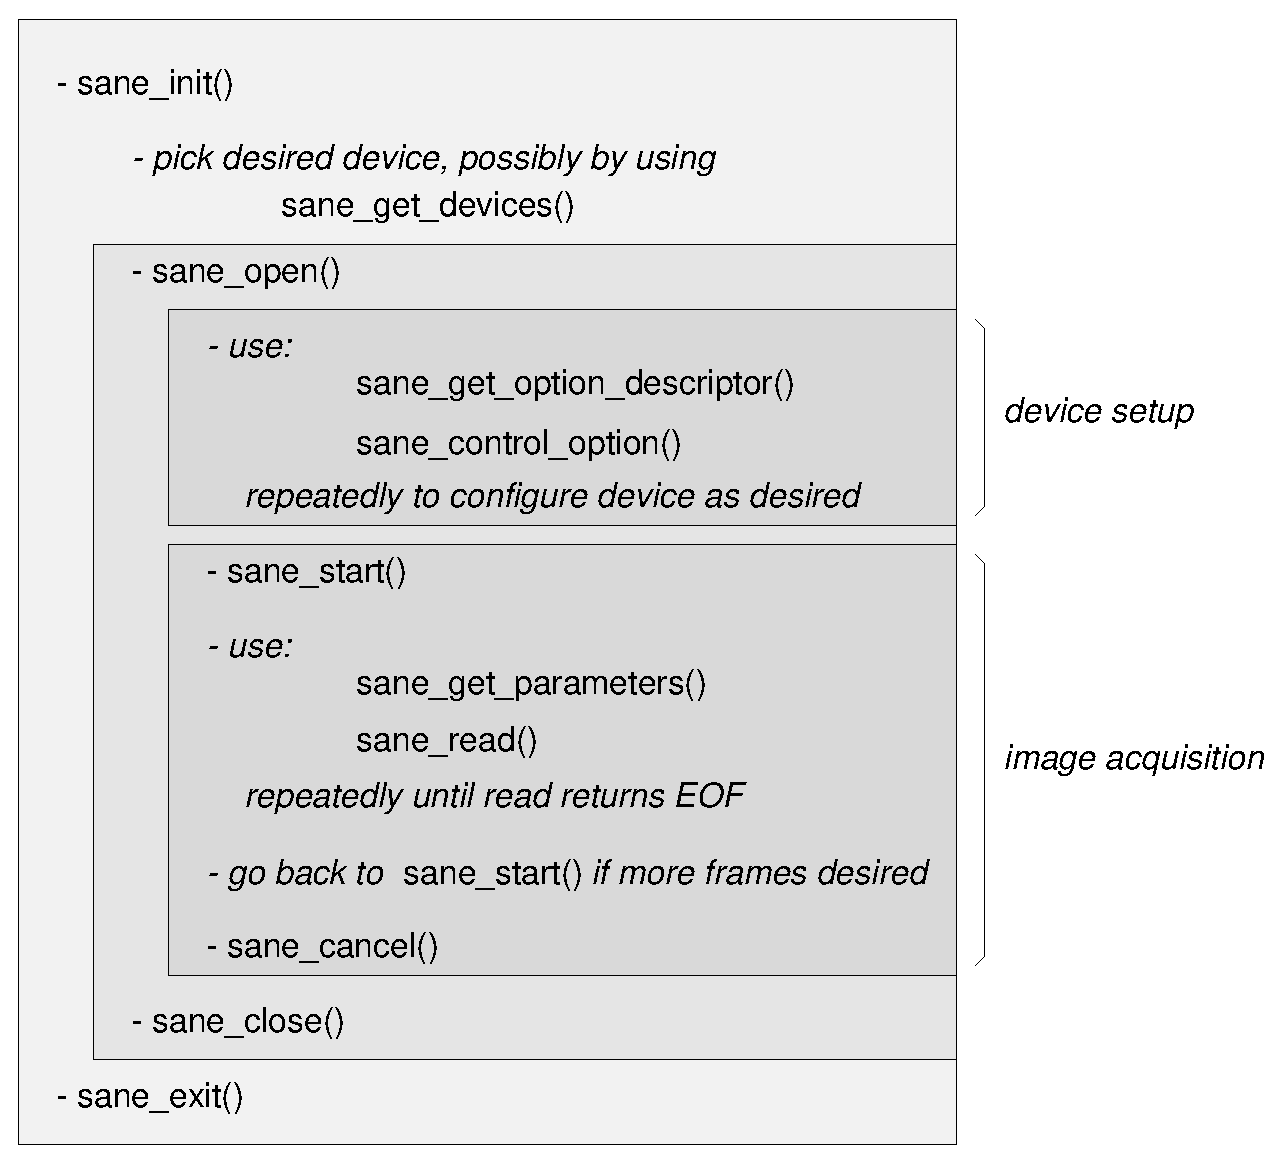
\psfig{file=figs/flow.eps,height=0.5\textheight}
    \caption{Code flow}
    \label{fig:flow}
  \end{center}
\end{figure}

Function \code{sane\_get\_devices()} can be called any time after
\code{sane\_init()} has been called.  It returns the list of the
devices that are known at the time of the call.  This list may change
over time since some devices may be turned on or off or a remote host
may boot or shutdown between different calls.  It should be noted that
this operation may be relatively slow since it requires contacting all
configured devices (some of which may be on remote hosts).  A frontend
may therefore want to provide the ability for a user to directly
select a desired device without requiring a call to this function.

Once a device has been chosen, it is opened using a call to
\code{sane\_open()}.  Multiple devices can be open at any given time.
A SANE backend must not impose artificial constraints on how many
devices can be open at any given time.

An opened device can be setup through the corresponding device handle
using functions \code{sane\_get\_opt\-ion\_desc\-riptor()} and
\code{sane\_control\_option()}.  While setting up a device, obtaining
option descriptors and setting and reading of option values can be
mixed freely.  It is typical for a frontend to read out all available
options at the beginning and then build a dialog (either graphical or
a command-line oriented option list) that allows to control the
available options.  It should be noted that the number of options is
fixed for a given handle.  However, as options are set, other options
may become active or inactive.  Thus, after setting an option, it
maybe necessary to re-read some or all option descriptors.  While
setting up the device, it is also admissible to call
\code{sane\_get\_parameters()} to get an estimate of what the image
parameters will look like once image acquisition begins.

The device handle can be put in blocking or non-blocking mode by a
call to \code{sane\_set\_io\_mode()}.  Devices are required to support
blocking mode (which is the default mode), but support for
non-blocking I/O is strongly encouraged for operating systems such as
UNIX.

After the device is setup properly, image acquisition can be started
by a call to \code{sane\_start()}.  The backend calculates the exact
image parameters at this point.  So future calls to
\code{sane\_get\_parameters()} will return the exact values, rather
than estimates.  Whether the physical image acquisition starts at this
point or during the first call to \code{sane\_read()} is unspecified
by the SANE API.  If non-blocking I/O and/or a select-style interface
is desired, the frontend may attempt to call
\code{sane\_set\_io\_mode()} and/or \code{sane\_get\_select\_fd()} at
this point.  Either of these functions may fail if the backend does
not support the requested operation.

Image data is collected by repeatedly calling \code{sane\_read()}.
Eventually, this function will return an end-of-file status
(\code{SANE\_STATUS\_EOF}).  This indicates the end of the current
frame.  If the frontend expects additional frames (e.g., the
individual channels in of a red/green/blue image or multiple images),
it can call \code{sane\_start()} again.  Once all desired frames have
been acquired, function \code{sane\_cancel()} must be called.  This
operation can also be called at any other time to cancel a pending
operation.  Note that \code{sane\_cancel()} must be called even if the
last read operation returned \code{SANE\_STATUS\_EOF}.

When done using the device, the handle should be closed by a call to
\code{sane\_close()}.  Finally, before exiting the application,
function \code{sane\_exit()} must be called.  It is important not to
forget to call this function since otherwise some resources (e.g.,
temporary files or locks) may remain unclaimed.


\section{Well-Known Options}\index{well-known options}

While most backend options are completely self-describing, there are a
cases where a user interface might want to special-case the handling
of certain options.  For example, the scan area is typically defined
by four options that specify the top-left and bottom-right corners of
the area.  With a graphical user interface, it would be tedious to
force the user to type in these four numbers.  Instead, most such
interfaces will want to present to the user a preview (low-resolution
scan) of the scanner surface and let the user pick the scan area by
dragging a rectangle into the desired position.  For this reason, the
SANE API specifies a small number of option names that have
well-defined meanings.

\subsection{Option Number Count}\index{option count}

Option number 0 has an empty string as its name.  The value of this
option is of type \code{SANE\_TYPE\_INT} and it specifies the total
number of options available for a given device (the count includes
option number 0).  This means that there are two ways of counting the
number of options available: a frontend can either cycle through all
option numbers starting at one until
\code{sane\_get\_option\_descriptor()} returns \code{NULL}, or a
frontend can directly read out the value of option number 0.

\subsection{Scan Resolution Option}\index{scan resolution}\index{resolution option}

Option \code{resolution} is used to select the resolution at which an
image should be acquired.  The type of this option is either
\code{SANE\_TYPE\_INT} or \code{SANE\_TYPE\_FIXED}.  The unit is
\code{SANE\_UNIT\_DPI} (dots/inch).

This option is not mandatory, but if a backend does support it, it
must implement it in a manner consistent with the above definition.

\subsection{Preview Mode Option}\index{preview mode}

The boolean option \code{preview} is used by a frontend to inform the
backend when image acquisition should be optimized for speed, rather
than quality (``preview mode'').  When set to \code{SANE\_TRUE},
preview mode is in effect, when set to \code{SANE\_FALSE} image
acquisition should proceed in normal quality mode.  The setting of
this option \emph{must not\/} affect any other option.  That is, as
far as the other options are concerned, the preview mode is completely
side effect free.  A backend can assume that the frontend will take
care of appropriately setting the scan resolution for preview mode
(through option \code{resolution}).  A backend is free to override the
\code{resolution} value with its own choice for preview mode, but it
is advised to leave this choice to the frontend wherever possible.

This option is not mandatory, but if a backend does support it, it
must implement it in a manner consistent with the above definition.

\subsection{Scan Area Options}\index{scan area options}

The four most important well-known options are the ones that define
the scan area.  The scan area is defined by two points (x/y coordinate
pairs) that specify the top-left and the bottom-right corners.  This
is illustrated in Figure~\ref{fig:area}.  Note that the origin of the
coordinate system is at the top-left corner of the scan surface as
seen by the sensor (which typically is a mirror image of the scan
surface seen by the user).  For this reason, the top-left corner is
the corner for which the abscissa and ordinate values are
simultaneously the {\em smallest} and the bottom-right corner is the
corner for which the abscissa and ordinate values are simulatenously
the {\em largest}.  If this coordinate system is not natural for a
given device, it is the job of the backend to perform the necessary
conversions.
\begin{figure}[tbp]
  \begin{center}
    \leavevmode
    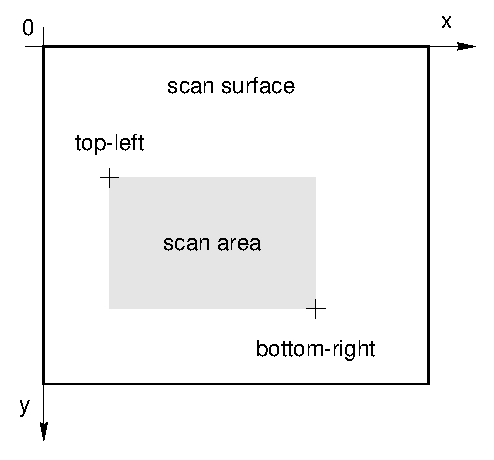
\psfig{file=figs/area.eps,height=0.3\textheight}
    \caption{Scan area options}
    \label{fig:area}
  \end{center}
\end{figure}

The names of the four options that define the scan area are given in
the table below:
\begin{center}
\begin{tabular}{ll}
{\bf Name} & {\bf Description} \\
\code{\defn{tl-x}} & Top-left $x$ coordinate value \\
\code{\defn{tl-y}} & Top-left $y$ coordinate value \\
\code{\defn{br-x}} & Bottom-right $x$ coordinate value \\
\code{\defn{br-y}} & Bottom-right $y$ coordinate value \\
\end{tabular}
\end{center}
There are several rules that should be followed by front and backends
regarding these options:
\begin{itemize}

\item Backends must attach a unit of either pixels
  (\code{SANE\_UNIT\_PIXEL}) or millimeters (\code{SANE\_UNIT\_MM}) to
  these options.  The unit of all four options must be identical.

\item Whenever meaningful, a backend should attach a range or a
  word-list constraint to these options.

\item A frontend can determine the size of the scan surface by first
  checking that the options have range constraints associated.  If a
  range or word-list constraints exist, the frontend can take the
  minimum and maximum values of one of the x and y option
  range-constraints to determine the scan surface size.

\item A frontend must work properly with any or all of these options
  missing.
  
\end{itemize}

\input{net.tex}

\chapter{Contact Information}\label{chap:contact}

The SANE standard is discussed and evolved via a mailing list.
Anybody with email access to the Internet can automatically join and
leave the discussion group by sending mail to the following address.
\begin{quote}\index{mailing list}
\begin{verbatim}
majordomo@mostang.com
\end{verbatim}
\end{quote}
To subscribe, send a mail with the body ``\verb|subscribe sane-devel|'' to the
above address.

A complete list of commands supported can be obtained by sending a
mail with a subject of ``\code{help}'' to the above address.  The
mailing list is archived and available through the SANE home page at
URL:
\begin{quote}
\url{http://www.mostang.com/sane/}
\end{quote}

\newpage
\input{sane.ind}

\end{document}


\end{document}


\end{document}


\end{document}
